%%%%%%%%%%%%%%%%%%%%%%%%%%%%%%%%%%%%%%%%%%%%%%%%%%%%%%%%%%%%%%%%%%%%%%
% njuthesis 示例模板 v1.4.2 2024-11-08
% https://github.com/nju-lug/NJUThesis
%
% 贡献者
% Yu XIONG @atxy-blip   Yichen ZHAO @FengChendian
% Song GAO @myandeg     Chang MA @glatavento
% Yilun SUN @HermitSun  Yinfeng LIN @linyinfeng
% Yukai Chou @Muzimuzhi
%
% 许可证
% LaTeX Project Public License(版本 1.3c 或更高)
%%%%%%%%%%%%%%%%%%%%%%%%%%%%%%%%%%%%%%%%%%%%%%%%%%%%%%%%%%%%%%%%%%%%%%

%---------------------------------------------------------------------
% 一些提升使用体验的小技巧:
%   1. 请务必使用 UTF-8 编码编写和保存本课题档
%   2. 请务必使用 XeLaTeX 或 LuaLaTeX 引擎进行编译
%   3. 不保证接口稳定,写作前一定要留意版本号
%   4. 以百分号(%)开头的内容为注释,可以随意删除
%---------------------------------------------------------------------

%---------------------------------------------------------------------
% 请先阅读使用手册:
% http://mirrors.ctan.org/macros/unicodetex/latex/njuthesis/njuthesis.pdf
%---------------------------------------------------------------------

\documentclass[
    % 模板选项(注意右端逗号):
    %
    % type = bachelor|master|doctor|postdoc, % 文档类型,默认为本科生
    % degree = academic|professional,        % 学位类型,默认为学术型
    %
    % nl-cover,   % 是否需要国家图书馆封面,默认关闭
    % decl-page,  % 是否需要诚信承诺书或原创性声明,默认关闭
    %
    %   页面模式,详见手册说明
    % draft,                  % 开启草稿模式
    % anonymous,              % 开启盲审模式
    % minimal,                % 开启最小化模式
    %
    %   单双面模式,默认为适合印刷的双面模式
    % oneside,                % 单面模式,无空白页
    % twoside,                % 双面模式,每一章从奇数页开始
    %
    %   字体设置,不填写则自动调用系统预装字体,详见手册
    % fontset = win|mac|macoffice|fandol|none,
  ]{njuthesis}

% 模板选项设置,包括个人信息、外观样式等
% 较为冗长且一般不需要反复修改,我们把它放在单独的文件里
% njuthesis 参数设置文件 v1.4.1 2024-04-19

% 一些提醒:
%   1. \njusetup 内部千万不要有空行
%   2. 使用英文半角逗号(,)分隔选项
%   3. 等于号(=)两侧的空格会被忽略
%       3.1. 为避免歧义,请用花括号({})包裹内容
%   4. 本科生无需填写的项目已被特别标注
%   5. 可以尽情删除本注释

% info 类用于录入个人信息
%   带*号的为对应英文字段
\njusetup[info]{
    title = {基于ChatGLM的文言文翻译模型的研究},
    % 中文题目
    % 直接填写标题就是自动换行
    % 可以使用换行控制符(\\)手动指定换行位置
    %
    title* = {Research on a Classical Chinese Translation Model Based on ChatGLM},
    % 英文题目
    %
    author = {汪博文},
    % 作者姓名
    %
    author* = {Bowen Wang},
    % 作者英文姓名
    % 一般使用拼音
    %
    keywords = {大语言模型,文言文-现代文翻译,ChatGLM3-6B模型},
    % 中文关键词列表
    % 使用英文半角逗号(,)分隔
    %
    keywords* = {Large Language Model, Classical Chinese-Modern Chinese translation, ChatGLM3-6B model},
    % 英文关键词
    % 使用英文半角逗号(,)分隔
    %
    grade = {2020},
    % 年级
    %
    student-id = {201250171},
    % 学号或工号
    % 研究生请斟酌大小写字母格式
    % 本模板并不会自动更正大小写
    %
    department = {软件学院},
    department* = {Software Institute},
    % 院系
    %
    major = {软件工程},
    major* = {Software Engineering},
    % 专业
    %
    % major = {封面专业,摘要专业},
    % 研究生专业型学位可能遇到两处内容不一致的情况
    %
    supervisor = {葛季栋,副教授},
    supervisor*= {Associate Professor Jidong GE},
    % 导师全称
    % 使用英文半角逗号(,)分隔中文姓名和职称
    %
    % supervisor-ii = {第二导师姓名,副教授},
    % supervisor-ii* = {Associate professor My Second Supervisor},
    % 第二导师全称
    % 如果确实没有第二导师,不填写即可
    %
    submit-date = {2024-06-02},
    % 提交日期
    % 格式为 yyyy-mm-dd
    % 不填就是编译当天日期
    %
    %
    % 以下均为研究生项
    %
    % degree = {工程硕士},
    % degree* = {Master of Engineering},
    % 覆盖默认学位名称
    %
    field = {物理化学},
    field* = {Physical Chemistry},
    % 研究领域
    %
    chairman = {某某某~教授},
    % 答辩委员会主席
    % 推荐使用波浪号(~)分隔姓名和职称
    %
    reviewer = {
        某某某~教授,
        某某某~教授
    },
    %
    % 答辩委员会成员
    % 一般为四名,使用英文半角逗号(,)分隔
    %
    clc = {O643.12},
    % 中国图书分类号
    %
    udc = {544.4},
    % 国际图书分类号
    %
    secret-level = {公开},
    % 密级
    %
    defend-date = {2022-05-21},
    % 答辩日期
    % 格式为 yyyy-mm-dd
    % 不填就是编译当天日期
    %
    email = {xyz@smail.nju.edu.cn},
    % 电子邮箱地址
    % 只用于出版授权书
    %
    %
    % 以下用于国家图书馆封面
    confer-date = {2022-05-22},
    % 学位授予日期
    %
    bottom-date = {2022-05-23},
    % 封面底部日期
    %
    supervisor-contact = {
        南京大学~
        江苏省南京市栖霞区仙林大道163号
    }
    % 导师联系方式
}

% bib 类用于参考文献设置
\njusetup[bib]{
    % style = numeric|author-year,
    % 参考文献样式
    % 默认为顺序编码制(numeric)
    % 可选著者-出版年制(author-year)
    %
    resource = {njuthesis-sample.bib},
    % 参考文献数据源
    % 需要带扩展名的完整文件名
    % 可使用逗号分隔多个文件
    % 此条等效于 \addbibresource 命令
    %
    % option = {
        % doi    = false,
        % isbn   = false,
        % url    = false,
        % eprint = false,
        % 关闭部分无用文献信息
        %
        % refsection = chapter,
        % 将参考文献表置于每章后
        %
        % gbnamefmt = lowercase
        % 使用仅首字母大写的姓名
    %   }
    % 额外的 biblatex 宏包选项
}

% image 类用于载入外置的图片
\njusetup[image]{
    % path = {{./figure/}{./image/}},
    % 图片搜索路径
    %
    nju-emblem = {nju-emblem},
    nju-name = {nju-name},
    % 校徽和校名图片路径
    % 建议使用 PDF 格式的矢量图
    % 使用外置图片有助于减少编译时间
    % 空置时会自动使用 njuvisual 宏包绘制
    %
    % nju-emblem = {nju-emblem-purple},
    % nju-name = {nju-name-purple},
    % 替换为紫色版本
    % 这个选项只能填写一次
    % 切换时要注释掉上方的黑色版本
}

% abstract 类用于设置摘要样式
\njusetup[abstract]{
    toc-entry = false,
    % 摘要是否显示在目录条目中
    %
    % underline = false,
    % 研究生英文摘要页条目内容是否添加下划线
    %
    % title-style = strict|centered|natural
    % 研究生摘要标题样式,详见手册
}

% 目录自身是否显示在目录条目中
\njusetup{
    tableofcontents/toc-entry = false,
    % 关闭本项相当于同时关闭三个选项
    %
    % listoffigures/toc-entry   = false,
    % listoftables/toc-entry    = false
}

% 为目录中的章标题添加引导线
\njusetup[tableofcontents/dotline]{chapter}

% math 类用于设置数学符号样式,功能详见手册
\njusetup[math]{
    % style              = TeX|ISO|GB,
    % 整体风格,缺省值为国标(GB)
    % 相当于自动设置以下若干项
    %
    % integral           = upright|slanted,
    % integral-limits    = true|false,
    % less-than-or-equal = slanted|horizontal,
    % math-ellipsis      = centered|lower,
    % partial            = upright|italic,
    % real-part          = roman|fraktur,
    % vector             = boldfont|arrow,
    % uppercase-greek    = upright|italic
}

% theorem 类用于设置定理类环境样式,功能详见手册
\njusetup[theorem]{
    % define,
    % 默认创建内置的七种定理环境
    %
    % style         = remark,
    % header-font   = \sffamily \bfseries,
    % body-font     = \normalfont,
    % qed-symbol    = \ensuremath { \male },
    % counter       = section,
    % share-counter = true,
    % type          = {...}
    % 以上设置项在重新调用 theorem/define 后生效
}

% footnote 类用于设置脚注样式,功能详见手册
\njusetup[footnote]{
  % style = pifont|circled,
  % 使用圈码编号
  %
  % hang = false,
  % 不使用悬挂缩进
}

% 页眉页脚内容设置
\njusetup{
  % header/content = {
  %     {OR}{\thepage},{OL}{\rightmark},
  %     {EL}{\thepage},{ER}{\leftmark}
  %   },
  % 页眉设置,详见手册
  % 奇数页页眉:左侧章名,右侧页码
  % 偶数页页眉:左侧页码,右侧节名
  %
  % footer/content = {}
}

% 页眉页脚的字体样式
% \njusetformat{header}{\small\kaishu}
% \njusetformat{footer}{}

% 在盲审模式下隐藏学校信息
% \njusetup{anonymous-mode/no-nju}

% 一些灵活调整
% \njusetname{type}{本科毕业设计}                 % 我做的是毕业设计
% \njusetname{notation}{术语表}                   % 更改符号表名称
% \njusetlength{crulewd}{240pt}                   % 加长封面页下划线
% \njusetformat{tabular}{\zihao{-4}\bfseries}     % 修改表格环境的字号
% \EditInstance{nju}{u/cover/emblem-img}{align=l} % 左对齐的本科生封面校徽


% 自行载入所需宏包
% \usepackage{subcaption} % 嵌套小幅图像,比 subfig 和 subfigure 更新更好
% \usepackage{siunitx} % 标准单位符号
% \usepackage{physics} % 物理百宝箱
% \usepackage[version=4]{mhchem} % 绘制分子式
\usepackage{listings} % 展示代码
\usepackage[dvipsnames]{xcolor}
% \usepackage{algorithm,algorithmic} % 展示算法伪代码
\usepackage{float}
% 在导言区随意定制所需命令
% \DeclareMathOperator{\spn}{span}
% \NewDocumentCommand\mathbi{m}{\textbf{\em #1}}

\renewcommand{\lstlistingname}{代码}
% \lstdefinestyle{pycharm}{
%     language=Python,
%     backgroundcolor=\color{white},
%     basicstyle=\footnotesize\ttfamily,
%     keywordstyle=\color{blue},
%     stringstyle=\color{green!40!black},
%     commentstyle=\color{gray}\emph,
%     frame=single,
%     numbers=left,
%     numberstyle=\tiny\color{gray},
%     captionpos=b,
%     breaklines=true,
%     breakatwhitespace=true,
%     tabsize=4,
%     showstringspaces=false,
%     extendedchars=true,
%     inputencoding=utf8,
%     escapeinside={\%*}{*)},
% }
\lstset{
    language=SQL,
    backgroundcolor=\color{white},
    basicstyle=\footnotesize\ttfamily,
    keywordstyle=\color{blue},
    stringstyle=\color{green!40!black},
    commentstyle=\color{gray}\emph,
    identifierstyle=\color{black},
    morekeywords={SELECT, FROM, WHERE, INSERT, UPDATE, DELETE, CREATE, ALTER, DROP, TABLE, 
                  JOIN, LEFT, RIGHT, INNER, OUTER, GROUP, ORDER, BY, HAVING, 
                  AS, ON, AND, OR, NOT, NULL, IS, IN, BETWEEN, LIKE, COUNT, SUM, AVG, MAX, MIN},
    frame=single,
    numbers=left,
    numberstyle=\tiny\color{gray},
    captionpos=b,
    breaklines=true,
    breakatwhitespace=true,
    tabsize=4,
    showstringspaces=false,
    extendedchars=true,
    inputencoding=utf8,
    escapeinside={\%*}{*)},
}


% 开始编写论文
\begin{document}

%---------------------------------------------------------------------
%	封面、摘要、前言和目录
%---------------------------------------------------------------------

% 生成封面页
\maketitle

% 模板默认使用 \flushbottom,即底部平齐
% 效果更好,但可能出现 underfull \vbox 信息
% 以下命令用于抑制这些信息
\raggedbottom

\begin{abstract}
产品质量是工业制造的基础,随着工业制造智能化的发展,对于产品质量检测的高效性与准确性的要求越来越高,而缺陷检测正是工业产品质量检测中不可或缺的一环,它保障了如金属、芯片、纺织物等各种工业制品的质量。

众所周知,传统的人工检测方法存在效率低、成本高、稳定性差等缺点,注定会被更高效、经济的检测方法所替代。近年来,随着计算机视觉、工业成像、深度学习等领域的兴起,基于视觉的工业缺陷检测取得了重大突破,也为检测方法的更新迭代提供了可能——构建神经网络训练样本并提取其特征,以实现自动化缺陷检测。最初,基于有监督深度学习的缺陷检测需要大量带标注的缺陷数据,这些标注数据不仅难以获得、成本高,且泛化能力弱,已不能满足当前主流的工业生产需求,于是基于无监督深度学习的缺陷检测方法应运而生。

无监督学习仅依据正常样本进行,通过挖掘特征实现对缺陷的识别,无疑更适合复杂的工业场景,逐渐成为研究的热点。然而,现有的无监督系统通常存在样本与模型缺乏管理、检测流程及参数配置复杂、辅助信息有限、界面布局混乱以及功能模块割裂等问题,难以满足工业场景快速部署的需求。因此,本课题基于开源项目 SimpleNet 和 AnomalyGPT,结合工业检测实际需求,设计并实现了集样本管理、模型训练、缺陷检测模块于一体的基于无监督学习的缺陷检测系统,旨在降低对标注数据的依赖,提高检测的灵活性,同时通过模块化设计与功能优化,提升系统的易用性与适应性。具体研究内容如下:

1. 针对样本类型多种多样、样本数量稀缺、样本质量参差不齐等问题,本课题设计了由动态样本组管理、数据增强与样本编辑操作等部分构建的样本组管理模块。

2. 针对自监督缺陷检测依赖大量标注数据、模型训练参数设置复杂,以及系统模型管理困难等问题,本课题设计了由无监督学习模型可视化训练、用户导向的参数映射与模型状态管理等部分构建的模型训练模块。其中,参数映射是将复杂的模型参数配置简化为"精度-速度-缺陷大小"的直观选项,以降低操作门槛。

3. 针对检测结果仅通过阈值判定、检测结果单一、辅助信息有限等问题,本课题设计了由无监督学习模型缺陷检测、大型视觉语言模型辅助判定与交互、检测分析与报告等部分构建的缺陷检测模块。系统通过热图可视化、大模型交互与检测报告,为工艺优化提供支持,具有一定的工业落地价值。
\end{abstract}

\begin{abstract*}
Product quality is the foundation of industrial manufacturing. With the development of intelligent industrial manufacturing, there is an increasing demand for efficiency and accuracy in product quality inspection. Defect detection is an indispensable part of industrial product quality inspection, ensuring the quality of various industrial products such as metals, chips, textiles, etc. 

It is well known that traditional manual detection methods have disadvantages such as low efficiency, high cost, and poor stability, which will inevitably be replaced by more efficient and economical detection methods. In recent years, with the rise of computer vision, industrial imaging, deep learning and other fields, vision-based industrial defect detection has made significant breakthroughs, providing possibilities for updating detection methods—constructing neural network training samples and extracting their features to achieve automated defect detection. Initially, defect detection based on supervised deep learning required a large amount of annotated defect data, which was not only difficult to obtain, costly, but also had weak generalization ability, and could no longer meet the needs of current mainstream industrial production. Thus, defect detection methods based on unsupervised deep learning emerged. 

Unsupervised learning relies only on normal samples, identifying defects by mining features, which is undoubtedly more suitable for complex industrial scenarios and has gradually become a research hotspot. However, existing unsupervised systems often suffer from problems such as lack of sample and model management, complex detection processes and parameter configurations, limited auxiliary information, chaotic interface layouts, and fragmented functional modules, making it difficult to meet the rapid deployment needs in industrial scenarios. Therefore, based on the open-source projects SimpleNet and AnomalyGPT, and combined with practical industrial inspection requirements, this study designed and implemented a defect detection system based on unsupervised learning that integrates sample management, model training, and defect detection modules. It aims to reduce dependence on annotated data, improve detection flexibility, and enhance system usability and adaptability through modular design and functional optimization. The specific research contents are as follows:

1. Addressing issues of diverse sample types, scarce sample quantities, and varying sample quality, this study designed a sample group management module consisting of dynamic sample group management, data augmentation, and sample editing operations.

2. Addressing problems such as self-supervised defect detection's dependence on large amounts of annotated data, complex model training parameter settings, and difficult system model management, this study designed a model training module consisting of unsupervised learning model visualization training, user-oriented parameter mapping, and model state management. The parameter mapping simplifies complex model parameter configuration into intuitive options of "accuracy-speed-defect size" to lower the operational threshold.

3. Addressing problems such as detection results being determined only by thresholds, singular detection results, and limited auxiliary information, this study designed a defect detection module consisting of unsupervised learning model defect detection, large vision language model aided judgment and interaction, and detection analysis and reporting. The system provides support for process optimization through heat map visualization, large model interaction, and detection reports, having certain industrial application value.
\end{abstract*}

% 生成目录
\tableofcontents
% 生成图片清单
\listoffigures
% 生成表格清单
\listoftables

%---------------------------------------------------------------------
%	正文部分
%---------------------------------------------------------------------
\mainmatter

\chapter{引言}

\section{研究背景及意义}

在人类现代社会生活的各个方面,不论是衣食住行,亦或是晨昏四季,工业制品都无处不在。《中国制造 2025》行动纲领指出,建设制造强国任务艰巨而紧迫,需要加速推进信息化与工业化的深度融合,推进生产过程的智能化\cite{[1]}。众所周知,在工业制造智能化进程中,产品质量的把控始终是提升工业生产经济效益的关键环节,而这一环离不开产品的缺陷检测。通过缺陷检测能够有效把控产品质量、检测流水线机器的工作状态以及评估生产制造技术的优良,对提高产品质量和生产效率、降低生产成本有着至关重要的作用\cite{[2]}。因此,基于视觉的工业缺陷检测不仅有非常重要的研究价值,同时也拥有广阔的应用前景\cite{[1]}。在传统的工业生产过程,缺陷检测主要依靠人工视觉,不仅具有检测效率低、误检率和漏检率高、人工成本高、实时性差、主观误差高的缺点,还有接触损伤的风险\cite{[3]}。同时,在缺陷尺寸小于 0.5 mm 且无较大光学形变时,人眼检测不到缺陷信息,不适用于大规模工业生产的要求\cite{[4]}。

后来,随着计算机图像处理技术与视觉传感技术的突破,机器视觉有效地解决了缺陷检测中人工的弊端,凭借其高效率、高精度、低成本等优势在工业检测领域中被广泛研究\cite{[5]}。机器视觉检测技术是一种非接触式的自动检测技术,具有安全可靠、检测精度高、可在复杂的生产环境中长时间运行等优点,是实现工厂生产自动化和智能化的一种有效方法\cite{[6]}。因而机器视觉逐渐取代人工视觉,成为工业缺陷检测的主力。目前,基于机器视觉的缺陷检测技术已广泛应用于工业产品的质量检测、分类检测和包装检测等,涉及钢板、玻璃、印刷、电子、纺织品、零件、木材、钢轨、瓷砖等多种关系国计民生的行业和产品\cite{[7]}。

然而,基于规则的传统图像处理算法往往只适用于特定场景,对于纹理背景复杂、缺陷类型多样化的工业场景来说有待提升。随着深度学习的发展,有监督学习方法通过其理解和提取产品缺陷特征方面的优势,在检测精度和检测速度上取得了双重突破,但这类方法存在两个问题:一是工业场景中缺陷样本数量稀少,收集大量带标注的缺陷样本成本高昂;二是工业生产过程复杂,缺陷模式和类型变幻莫测,基于有监督学习的缺陷检测模型对未训练过的新型缺陷类型泛化能力不足,难以适应快速变化的生产工艺。

近年来,基于无监督学习的缺陷检测技术因其能自动学习潜在特征和模式,仅需正常样本即可完成训练的特性,逐渐成为研究热点。经研究发现,现有的无监督检测方法存在三个缺陷:第一,计算复杂度高,如部分基于生成对抗网络(GANs)的方法虽然检测精度较高,但运算开销大,难以满足工业实时检测需求;第二,参数配置专业性强,增加了工程部署门槛,不利于非专业用户使用;第三,检测结果信息量少,对于工业制造中的缺陷检测所能提供的辅助作用低下。此外,大多数现有方法仅提供异常评分而不能直接判断异常,需要人工设置阈值,这在动态变化的生产环境中缺乏灵活性。

本课题旨在对基于无监督深度学习的缺陷检测算法模型如何向实际工业应用进行转化,以及相应缺陷检测系统的设计与开发展开研究。结合已有的开源算法模型,设计一套面向工业实际应用场景的无监督缺陷检测系统,致力于解决训练数据稀缺且质量参差不齐、模型检测速度与精度难以平衡、模型参数配置复杂、检测效益低下等问题,提高检测效率与准确性,降低检测成本与学习成本,帮助优化生产工艺,从而提高产品质量,提升生产制造的效益,最终实现促进工业智能制造的发展的目标。

\section{国内外研究现状}

\subsection{工业缺陷检测技术}

工业缺陷检测技术经历了从人工检测到计算机视觉自动检测的发展历程。随着深度学习技术的发展,缺陷检测也经历了从传统图像处理方法到无监督深度学习方法的演进。本节将对工业缺陷检测方法的三个研究阶段展开介绍。

在深度学习技术尚未兴起之时,产品表面缺陷检测方法可划分为基于传统图像处理的方法和基于机器学习的方法\cite{[8]}。基于图像处理的缺陷检测主要分为图像预处理和缺陷检测两个部分,图像预处理包括图像去噪和图像分割等算法,是缺陷检测的前期工作,缺陷检测部分主要利用图像特征提取或模板匹配算法完成对缺陷的检测\cite{[6]}。基于机器学习的缺陷检测方法通常使用支持向量机(SVM)、随机森林(Random Forest)等算法对缺陷进行分类,取得了较好的缺陷识别和分类效果。然而,此类方法一般依赖于人为设定的环境,仅适用于简单场景和规则缺陷,无法直接应用于实际复杂的工业生产环境。

随着深度学习技术在机器视觉领域的发展,以卷积神经网络(CNN)为代表的深度学习方法开始占据工业缺陷检测领域的主导地位,缺陷检测不再需要手动提取特征。目前较为典型的基于深度学习的缺陷检测方法包括基于卷积神经网络的缺陷检测方法、基于深度信任网络(DBN)的缺陷检测方法、基于自编码器(AE)的缺陷检测方法等。其中,前两者属于有监督深度学习,后者属于无监督深度学习\cite{[6]}。有监督学习算法,如 Faster R-CNN、YOLO 系列算法在缺陷定位与分类中表现良好,但依赖大量标注数据,而工业领域中缺陷数据往往难以获取且成本高昂。

针对深度学习中缺陷样本过少的问题,基于无监督学习的缺陷检测方法被提出并逐步推广。无监督缺陷检测方法是利用正常样本训练,学习其分布模式,来检测缺陷的。它不依赖于标注数据,不受限于缺陷类型。根据数据处理与比较的维度不同,无监督方法可以分为基于图像相似度的方法和基于特征相似度的方法。前者包括自编码器(AE)、变分自编码器(VAE)和生成对抗网络(GAN)等,后者包括深度一类分类、流模型和教师-学生架构等\cite{[1]}。

\subsection{工业缺陷检测系统}

目前,基于深度学习的工业产品缺陷检测算法层出不穷,但市面上开源的工业缺陷检测系统却较为匮乏,且多数为特定产品的缺陷检测系统,难以满足工业质检的多样性需求,从科学研究到工业应用的转化需要进一步加强。

市面上商用的缺陷检测系统五花八门。HALCON 是德国 MVtec 公司开发的一款通用机器视觉软件,其应用范围涵盖自动化检测、医学和生命科学、遥感探测、通讯和监控等众多领域,被公认为具有最佳效能的机器视觉软件。HALCON 包含无监督深度学习异常检测模块,无需标注数据即可训练模型。其优势在于需要的图像少,速度快,每秒能够检测 40 次。但是,如图 \ref{HALCON} 所示,HALCON 的界面简陋、模块割裂、配置复杂,这也是市面上很多缺陷检测系统共同的缺点。

\begin{figure}[ht]
  \centering
  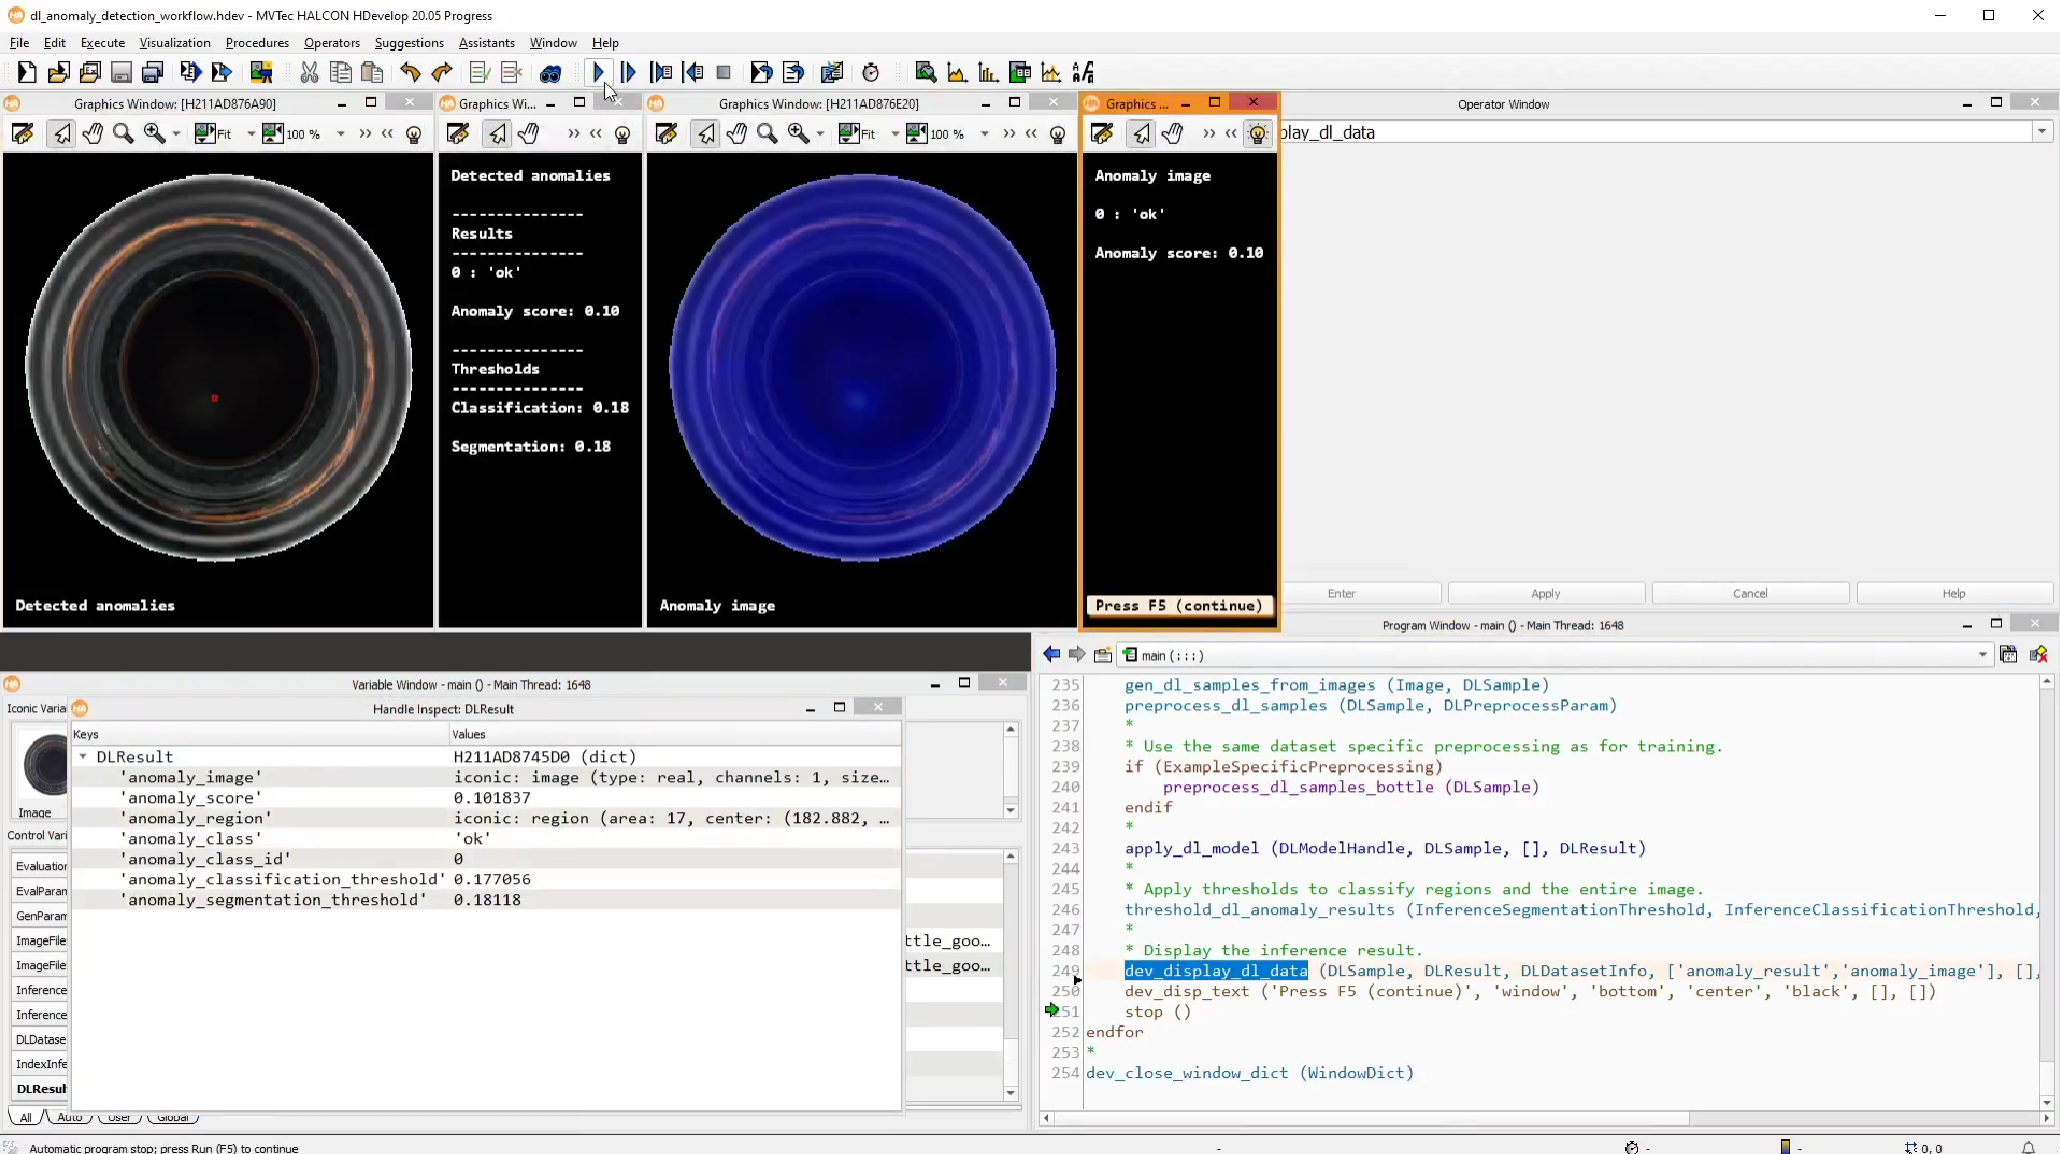
\includegraphics[width=\textwidth]{images/HALCON系统界面.png}
  \caption{HALCON系统进行缺陷检测的界面}
  \label{HALCON}
\end{figure}

因此,本课题设计并实现了一个开源的、跨平台的、目标产品多样化、用户友好的基于无监督深度学习的工业缺陷检测系统,以促进无监督缺陷检测技术的工业落地。

\section{研究内容与主要工作}

本课题围绕基于无监督学习的工业缺陷检测系统的设计与实现展开,使用无监督深度学习检测方法 SimpleNet 和缺陷检测大型视觉语言模型 AnomalyGPT,旨在解决现有系统在用户可用性及易用性、工程落地效益等方面的不足。本课题的主要工作分为以下六个部分:  

\begin{enumerate}
    \item 基于 SimpleNet 构建无监督缺陷检测框架,实现模型训练与检测核心功能。
    \item 基于 AnomalyGPT 实现视觉语言模型辅助判定与分析功能。
    \item 实现裁剪、缩小域、数据增强等训练样本预处理操作。
    \item 实现样本组和模型的管理,包括模型参数的动态配置。
    \item 实现缺陷检测报告功能,完善检测流程。
    \item 在实现上述功能的基础上,根据人机交互启发式原则,设计一个用户友好的系统。
\end{enumerate}

\section{论文组织结构}

本课题围绕无监督学习的缺陷检测系统的设计与实现展开,全文共分为六章,具体组织结构如下:  

第一章:\textit{引言}。阐述本课题的研究背景、研究意义、研究现状、研究内容及论文结构。

第二章:\textit{基本概念与相关工作}。介绍无监督异常检测的基本概念、系统开发相关的研究工作以及技术栈。

第三章:\textit{系统设计}。对研究项目进行总体描述与需求分析,并设计相应的系统架构和数据库。

第四章:\textit{系统实现}。介绍开发环境,详细说明系统核心模块、系统接口与其它实现,包括部署方式。

第五章:\textit{实验}。介绍数据集、实验设计,并对实验结果进行分析。

第六章:\textit{总结与展望}。总结本课题的成果,分析其局限性,对后续工作进行展望。 

\section{本章小结}

本章首先介绍了本课题的研究背景及意义,并调研了工业缺陷检测相关的国内外研究现状,然后总结了本课题在无监督缺陷检测系统的设计与实现方面的研究内容和主要工作,最后展示了本课题的整体组织结构。

\chapter{基本概念和相关工作}

\section{基本概念}

\subsection{缺陷与异常的概念}

缺陷是产品表面的物理瑕疵,如裂纹、划痕和凹陷,而异常是图像中不符合正常模式的部分,包括颜色、纹理或形状的异常变化\cite{[9]}。在工业上的缺陷检测中,缺陷通常被视作异常。因而,本课题中“缺陷”是指在实际生产过程中,由于生产设备、工艺流程、生产环境等各因素的影响,造成产品表面出现的各种异常\cite{[10]},如瓶底表面的裂纹、划痕,木板表面的磨损,皮革表面的污渍,螺母表面的锈迹等。这些缺陷不仅影响产品的外观,还可能影响其功能和使用寿命,甚至产生一系列安全隐患。

理论上缺陷检测系统是利用制品表面的光学物理性质,在特定的光学成像条件下,令缺陷表现出区别于背景的图像特征,然后通过图像处理技术和缺陷检测算法进行缺陷识别和定位\cite{[11]}。也就是说,完整的流程应该包括光学成像、图像预处理和缺陷检测三个部分,我们主要关注后两者。其中,图像预处理是指对采集的样本进行去噪、增强、分割、拼接等操作,将目标集中于感兴趣的区域,以提取缺陷区别于背景的特征。而缺陷检测在本课题中则是指使用基于无监督学习的缺陷检测算法进行缺陷识别和定位的过程。

缺陷标注样本是指人工标注出缺陷区域,并提供缺陷的类型、位置、大小等信息的用于模型训练的样本。它们大量使用于有监督学习中,但在工业场景中难以收集,且成本高昂。这也是无监督学习方法能够快速发展的重要原因。但是由于工业流程的不断优化,缺陷样本的数量在减少,在数据集较小的情况下,模型很难从有限的数据中学习到足够的特征,导致模型的泛化能力较差 \cite{[12]}。数据增强是目前解决这一问题的常用方法,它通过对初始样本进行一系列随机变换,如裁剪、缩放、旋转、平移等操作,生成新的样本,从而增加样本数量。

\section{SimpleNet}

\subsection{SimpleNet 概述}

SimpleNet\cite{[13]} 是中国科学技术大学提出的一个用于检测和定位图像异常区域的简单和应用友好的网络,它结合了合成型和嵌入型方法的优势,并做了一些改进:首先,使用特征适配器将预训练的特征转换为目标导向的特征以减少领域偏差,以适应工业产品图像。其次,在特征空间中向正常特征添加高斯噪声来生成合成异常,因为缺陷在图像空间中没有太多共性。简单来说就是工业缺陷表现形式多样,在图像层面难以找到统一的模式规律来合成逼真的缺陷,而在特征空间添加高斯噪声可以模拟各种特征偏移而不必关心具体缺陷形态。再者,通过简单的鉴别器来简化异常检测过程,提升计算效率。具体来说,如图 \ref{SimpleNet} 所示,在训练阶段,SimpleNet 先使用预训练的主干网络提取局部特征,然后通过特征适配器将特征转移到目标域,接着向正常特征添加高斯噪声以伪造异常特征,最后使用简单鉴别器训练特征并鉴别异常。

\begin{figure}[ht]
    \centering
    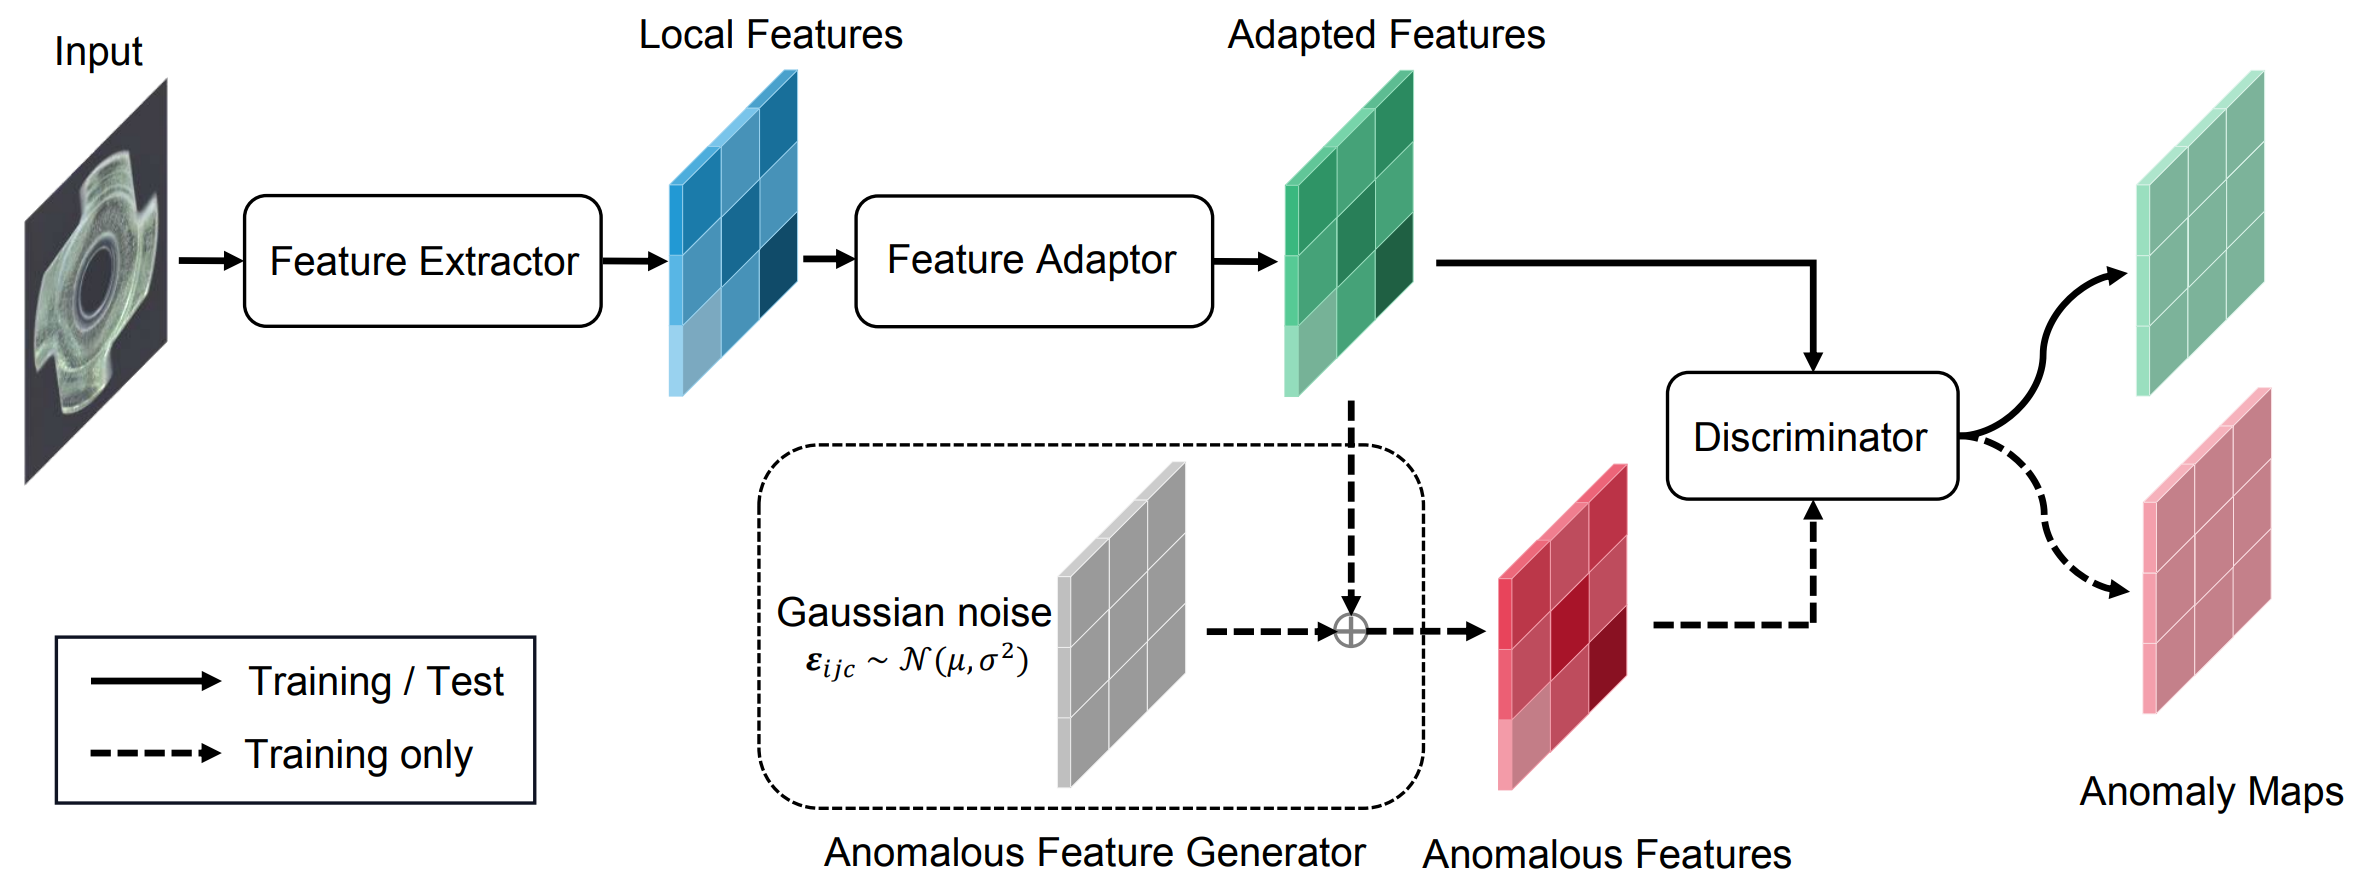
\includegraphics[width=0.88\textwidth]{images/SimpleNet概述.png}
    \caption{SimpleNet 概述}
    \label{SimpleNet}
\end{figure}

\subsection{SimpleNet 分析}

SimpleNet 能够检测到从细微变化到结构缺陷等不同程度的异常,适用于缺陷样本稀缺的工业场景。SimpleNet 在 MVTec AD 数据集上的异常检测中 AUROC 高达 99.6\%,并且准确性与效率均远远超过以前的所有方法,满足了工业质检的实时性和质量要求。综上所述,SimpleNet 具有优异的性能和推理速度,且易于训练和应用,因此本课题使用它来构建工业场景下的无监督缺陷检测系统。

\section{AnomalyGPT}

\subsection{AnomalyGPT 概述}

AnomalyGPT\cite{[14]} 是中国科学院提出的一种基于大型视觉语言模型(LVLMs)的工业异常检测(IAD)方法。如图 \ref{AnomalyGPT比较图} 所示,现有的 IAD 方法和 LVLMs 都不能很好地解决工业异常检测问题,比如前者只能提供异常分数,需要手动设置阈值,后者无法检测图像中的异常。而 AnomalyGPT 使用合成的异常视觉文本数据对 LVLM 进行微调,将 IAD 知识集成到模型中,加强了对图像内部细节的理解,不仅能提供图像信息,还能指示异常的存在和位置。作为第一个成功将 LVLM 应用到工业异常检测领域的方法,AnomalyGPT 的贡献如下:(1)无需手动调整阈值即可检测和定位异常,且支持多轮对话。(2)设计了一个轻量级的视觉文本特征匹配解码器,解决了大语言模型无法识别细粒度图像细节的问题,同时突破了输出形式的限制,以热图、文本结合的方式提供更多元的信息。(3)采用提示嵌入(prompt embedding)进行微调,并使用缺陷检测数据和 LVLM 的预训练数据进行训练,从而保留了 LVLM 所固有的上下文理解和对话管理能力,以支持多轮对话。最后,模型具有很强的可移植性,通过上下文少样本学习,即可快速适应新数据集。

\begin{figure}[ht]
    \centering
    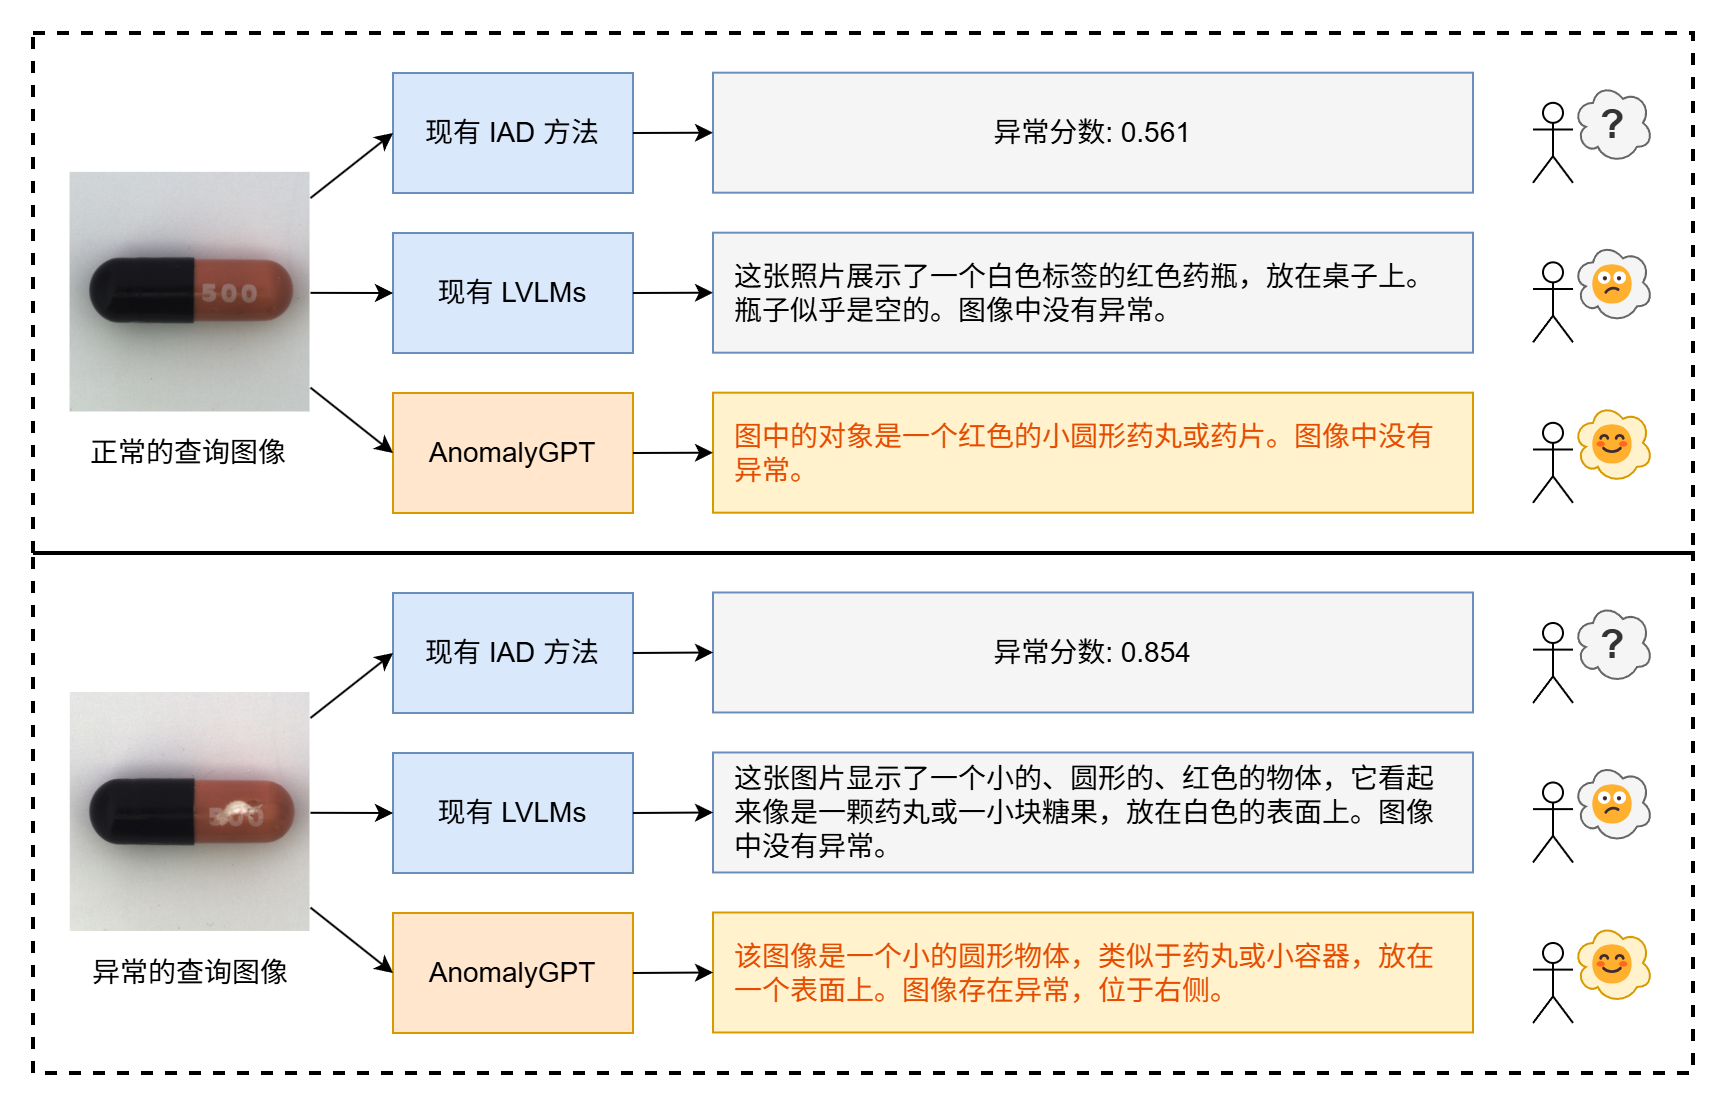
\includegraphics[width=0.75\textwidth]{images/AnomalyGPT演示.png}
    \caption{AnomalyGPT、现有 IAD 方法和现有 LVLMs 之间的比较}
    \label{AnomalyGPT比较图}
\end{figure}


\subsection{AnomalyGPT 分析}

大多数现有的 IAD 方法,包括 SimpleNet,仅提供测试样本的异常分数,需要手动设置阈值来区分正常和异常样本,这降低了缺陷检测系统的实际应用体验。因此,本课题引入了 AnomalyGPT。它不仅可以直接判定异常的存在并检测异常的位置,还可以提供图像相关信息,同时允许用户进行交互式问答,增强检测结果的可解释性和实用性。除此之外,AnomalyGPT 可以利用少量正常样本进行学习,从而快速适应新对象。在 MVTec AD 数据集上,AnomalyGPT 仅使用一个正常样本就能达到 86.1\% 的准确率、94.1\% 的图像级 AUC 和 95.3\% 的像素级 AUC。这些特性表明 AnomalyGPT 拥有良好的泛化能力,适合样本稀缺且缺陷多种多样的实际工业场景。

\section{技术栈}

\subsection{开发框架}

Qt 是 1991 年由 Qt Company 推出的一个跨平台的 C++ 图形用户界面(GUI)应用程序开发框架,可以用于 Windows、Linux、和 Mac OS 等桌面应用的开发,也可以用于 iOS、Android 等嵌入式应用开发。Qt 采用面向对象设计,易于扩展,支持组件编程。它提供了丰富的 API 接口,拥有活跃的社区,提供了各种文档和教程支持,能够帮助开发者快速入门。

PySide 是一个基于 Python 的图形用户界面库,它是由 C++ 版本的 Qt 库移植而来,提供了对 Qt 的完整访问,包括其核心模块、GUI组件、多媒体、网络、数据库等功能。PySide 和 PyQt 是同类产品,二者皆是 Qt 的 Python 版本,API 接口几乎一模一样,用法基本相同。不过,它们使用的协议不同,前者是 LGPL,可以免费用于商业用途,而后者是 GPL,只能免费用于个人用途。PySide 的优点是控件比较丰富、跨平台体验好、文档完善、用户多,适用于开发功能复杂的正式产品;缺点是库比较大,发布出来的应用程序体积较大。

Qt Designer 是 Qt 推出的一个用于图形化设计 GUI 界面的工具。通过拖放可视化的小控件,开发者可以轻松创建复杂的用户界面,不再需要编写代码。Qt Designer 不仅提高了 UI 界面的开发效率,还帮助开发者实现了视图和逻辑的解耦。这样一来,界面设计完成后,只需处理业务逻辑代码。

\subsection{数据库}

MySQL 是最流行的开源关系型数据库管理系统,它采用结构化查询语言(SQL)进行数据管理,支持 ACID 特性,适用于 Windows、Linux、MacOS 等多种操作系统。MySQL 具有体积小、速度快、成本低、可靠性高的特点,被广泛应用于各种网站和应用程序中。

\subsection{部署工具}

PyInstall 是一个跨平台的 Python 应用程序打包工具,它能自动检测 Python 脚本依赖的模块和库,包括资源文件,将它们打包成一个独立的可执行文件。

\subsection{其它}

OpenCV 是学术界和工业界广泛使用的一个开源的计算机视觉库,提供了丰富的图像处理和计算机视觉方面的通用算法,包括图像处理、特征提取、目标检测、图像分割、运动分析等。

Sobel 算子是经典的边缘检测算子,主要用于图像处理中识别图像的边缘特征。它采用两个 3x3 的卷积核来计算图像每个像素点在水平和垂直方向的灰度变化,变化较大的区域即边缘位置。Sobel 算子能提取产品表面的边缘信息,帮助使用者识别划痕等线性缺陷、分析纹理变化情况。

DBSCAN 是一种基于密度的聚类方法,该算法能够将给定的数据点划分为不同的簇,并且能够识别噪声点。它将簇定义为密度相连的点的最大集合,通过邻域半径 ε (Eps) 和最小样本数 MinPts 这两个参数来控制其生成。簇有三类点:核心点在其 ε 邻域内至少包含 MinPts 个样本点,边界点不是核心点但在某个核心点的邻域内,噪声点既不是核心点也不是边界点。

\section{本章小结}

本章介绍了工业缺陷检测的基本概念及相关技术。首先,阐述了与缺陷检测相关的概念,然后描述了 SimpleNet 方法和 AnomalyGPT 模型的工作原理及优势,最后介绍了系统的技术栈,包括开发框架、数据库、部署工具,以及系统所依赖的库和算法。

\chapter{系统设计}

\section{总体描述}

\subsection{系统目标}

本系统是工业质检的辅助工具,旨在帮助质检人员方便、快捷、直观地识别工业产品表面的缺陷,同时能够平衡检测精度和速度,满足各种尺寸的缺陷检测需要。作为一款跨平台的桌面应用程序,系统的前端使用 Qt 框架和 PySide6 库开发,后端采用 FastAPI 框架和 MySQL 数据库。系统主要分为样本管理模块、模型训练模块、缺陷检测和报告模块,具有样本编辑管理、模型可视化训练、实时缺陷检测、AI 辅助判别和自动报告生成等功能。

系统的核心算法基于 SimpleNet 和 AnomalyGPT,能够实现仅基于正常样本的无监督学习、缺陷检测和辅助分析。同时,系统应该尽量满足人机交互启发式原则,能够提供用户友好的界面,支持专业用户与业余用户操作。另外,系统应能够支持多线程,同时满足一定的数据处理效率。

\subsection{用户特征}

系统面向工业质检人员和从事无监督缺陷检测的研究人员,使用者希望通过系统更加高效地检测工业产品表面缺陷,提高工业质检效率,降低人工成本。其中,鉴于工业质检人员的工作特点,部分质检员可能具有多年视觉检测的工作经验,但对于深度学习模型原理和参数配置缺乏专业知识。同时,由于传统工业检测习惯根深蒂固,计算机辅助检测系统的使用存在一定门槛。而对于研究人员,他们可能需要更加灵活地配置系统参数,或获取详细的检测结果数据。综上所述,系统应尽可能地简化操作流程,提供直观的参数设置界面,同时为高需求的用户提供额外功能。这样一来,既满足了质检人员快速上手的需求,又能支持研究人员进行深入的算法优化与分析。

\section{需求分析}

\subsection{功能性需求}

(1)项目管理功能。用户可以创建、打开和管理缺陷检测项目,保存项目元数据和配置信息。此外,系统还提供历史项目快速访问功能,支持项目导航和拖放打开项目等操作,方便用户快速恢复之前的工作状态。

(2)样本管理功能。用户可以创建和管理多个样本组,批量导入和组织样本图像。系统支持图像预处理(裁剪、旋转、缩放)和数据增强(几何变换、亮度调整、颜色变换)。用户完成样本准备后,可将样本上传至服务器进行后续处理。

(3)模型训练功能。系统将参数(如嵌入维度、层数、补丁大小等)转换为"精度-速度-缺陷大小"等选项,用户可以直观地配置模型,不必知道算法内部的具体实现细节。模型训练时,过程可视化,系统实时显示训练进度和性能指标。

(4)缺陷检测功能。用户可以导入和管理待检测样本,使用已训练的模型执行缺陷检测。系统集成服务器检测能力,提供结果可视化功能,包括原图/热图切换、缺陷区域标记等。用户可调整检测阈值优化结果,并进行批量检测和结果存储。

(5)AI辅助分析功能。用户可通过自然语言交互界面对检测结果进行辅助分析。系统集成大型视觉语言模型的分析能力,支持多图像分析,包括说明缺陷是否存在(无需手动设置阈值)和缺陷位置,以及提供图像相关信息,使检测结果更具可解释性和实用价值。

(6)检测结果报告功能。用户可查看缺陷数据统计与分析结果,包括位置分布、聚类分析等多维度信息,以及对工艺改进的建议。系统自动生成检测报告,集成各类可视化图表,并支持导出为 PDF 格式,便于分享和存档。

系统用例图如图 \ref{系统用例图} 所示。

\begin{figure}[htb]
    \centering
    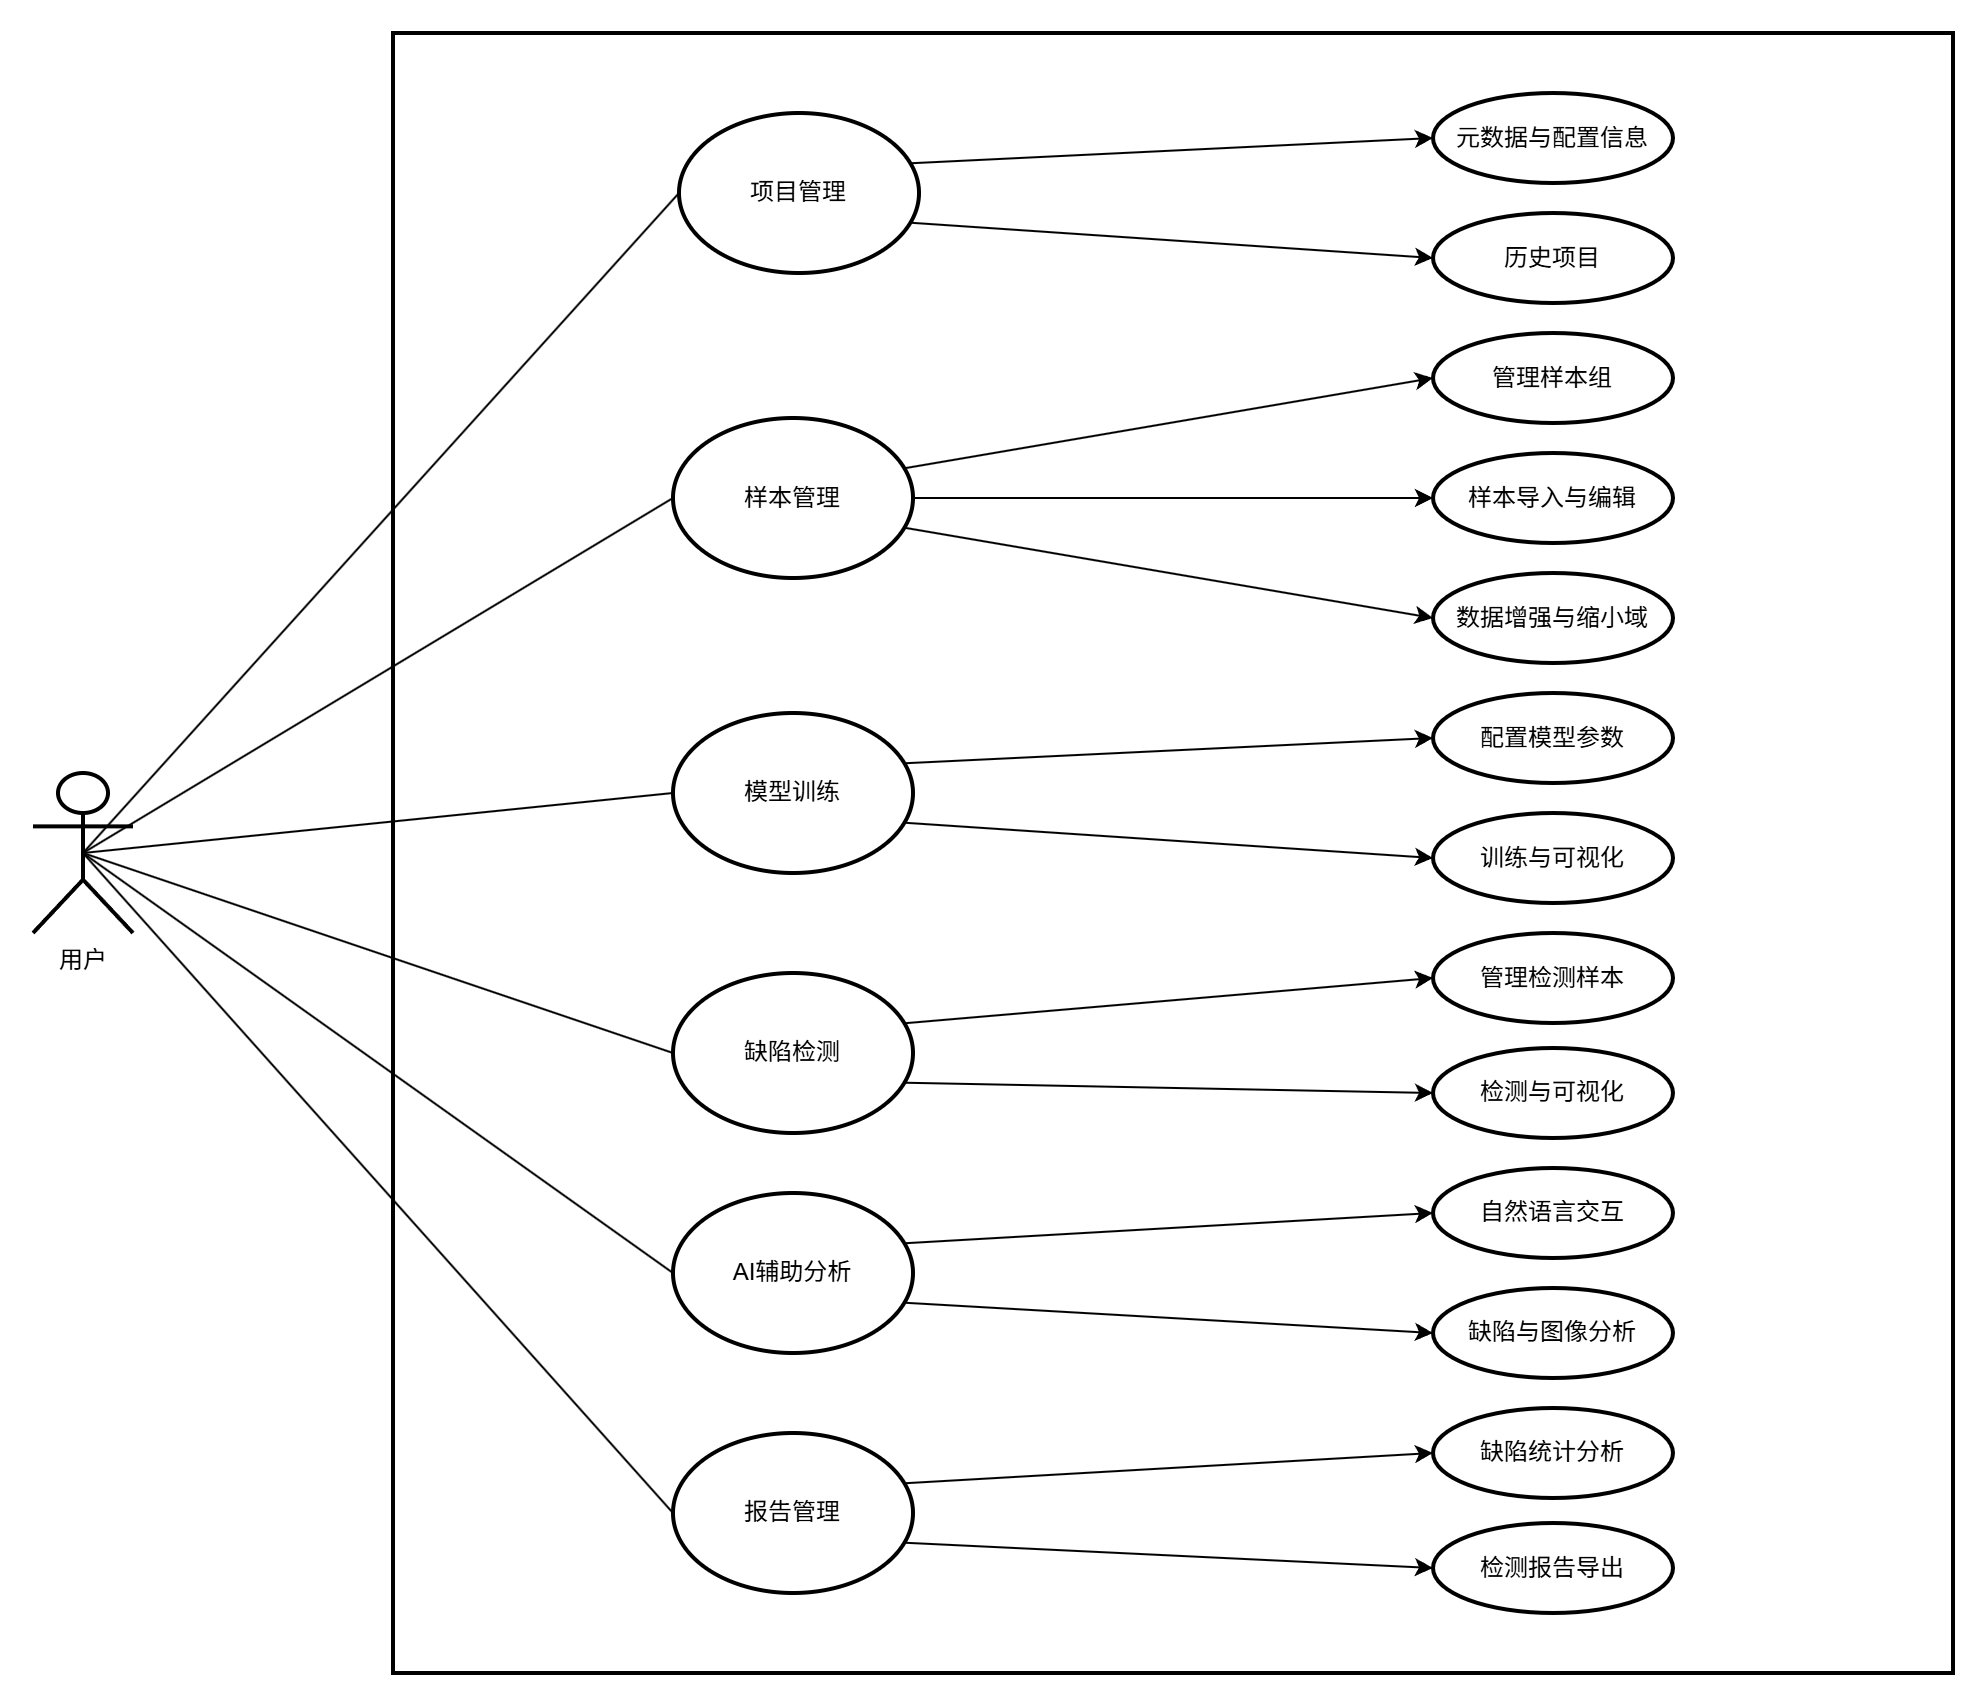
\includegraphics[width=\textwidth]{images/用例图.png}
    \caption{系统用例图}
    \label{系统用例图}
\end{figure}

\subsection{用例描述}

(1)用户在缺陷检测系统进行项目管理的用例描述如下表 \ref{usecase_project_management} 所示。

\begin{table}[H]
    \centering
    \caption{缺陷检测项目管理用例}
    \label{usecase_project_management}
    \renewcommand\arraystretch{0.5}
    \begin{tabular}{p{2.5cm}p{11cm}}
    \toprule[1.5pt]
    名称 & 内容描述 \\
    \midrule[1pt]
    ID & 01 \\
    \midrule[0.5pt]
    用例名称 & 项目管理 \\
    \midrule[0.5pt]
    参与者 & 用户 \\
    \midrule[0.5pt]
    描述 & 允许用户创建新项目、打开已有项目、管理项目元数据和配置信息 \\
    \midrule[0.5pt]
    触发条件 & 用户启动系统或选择项目管理功能 \\
    \midrule[0.5pt]
    前置条件 & 系统正常运行 \\
    \midrule[0.5pt]
    后置条件 & 创建项目或项目信息被用户修改时,系统自动保存 \\
    \midrule[0.5pt]
    优先级 & 低 \\
    \midrule[0.5pt]
    正常流程 & 1. 用户启动系统,显示项目管理界面 \newline
    2. 用户选择"新建项目"或"打开项目"或"最近项目" \newline
    3. 新建项目时,用户输入项目名称和存储位置 \newline
    4. 打开项目或最近项目时,用户选择本地存储的项目文件 \newline
    5. 系统加载项目,初始化配置信息 \\
    \midrule[0.5pt]
    扩展流程 & 3a. 如果项目名称已存在或非法,提示用户选择其他名称 \newline
    4a. 如果项目文件损坏,显示错误信息 \newline
    4b. 用户可通过拖放方式打开项目文件 \newline
    4c. 如果最近项目不存在,自动从历史列表中删除 \\
    \midrule[0.5pt]
    特殊需求 & 无 \\
    \bottomrule[1.5pt]
    \end{tabular}
\end{table}

(2)用户在模型训练前导入样本并进行管理的用例描述如下表 \ref{usecase_sample_management} 所示。

\begin{table}[H]
    \centering
    \caption{训练样本管理用例}
    \label{usecase_sample_management}
    \renewcommand\arraystretch{0.5}
    \begin{tabular}{p{2.5cm}p{11cm}}
    \toprule[1.5pt]
    名称 & 内容描述 \\
    \midrule[1pt]
    ID & 02 \\
    \midrule[0.5pt]
    用例名称 & 样本管理 \\
    \midrule[0.5pt]
    参与者 & 用户 \\
    \midrule[0.5pt]
    描述 & 允许用户创建样本组、导入样本图像、进行预处理和数据增强,以及上传至服务器 \\
    \midrule[0.5pt]
    触发条件 & 用户进入样本管理流程 \\
    \midrule[0.5pt]
    前置条件 & 已创建或打开项目 \\
    \midrule[0.5pt]
    后置条件 & 样本上传至服务器 \\
    \midrule[0.5pt]
    优先级 & 高 \\
    \midrule[0.5pt]
    正常流程 & 1. 用户创建新样本组或导入已有样本组 \newline
    2. 用户导入图像文件或文件夹 \newline
    3. 系统显示导入的样本列表 \newline
    4. 用户可选择图像进行裁剪、缩小域等预处理 \newline
    5. 用户可对样本进行数据增强或添加伪缺陷 \newline
    6. 用户将样本上传至服务器 \\
    \midrule[0.5pt]
    扩展流程 & 2a. 如果导入非图像文件,系统过滤不支持的文件 \newline
    4a. 用户可批量应用部分预处理操作 \newline
    6a. 大批量图像处理时显示进度条 \newline
    6b. 上传失败时显示错误信息 \\
    \midrule[0.5pt]
    特殊需求 & 无 \\
    \bottomrule[1.5pt]
    \end{tabular}
\end{table}

(3)用户在训练基于无监督学习的缺陷检测模型的用例描述如下表 \ref{usecase_model_training} 所示。

\begin{table}[H]
    \centering
    \caption{无监督学习模型训练用例}
    \label{usecase_model_training}
    \renewcommand\arraystretch{0.5}
    \begin{tabular}{p{2.5cm}p{11cm}}
    \toprule[1.5pt]
    名称 & 内容描述 \\
    \midrule[1pt]
    ID & 03 \\
    \midrule[0.5pt]
    用例名称 & 模型训练 \\
    \midrule[0.5pt]
    参与者 & 用户 \\
    \midrule[0.5pt]
    描述 & 允许用户配置和训练无监督缺陷检测模型,提供训练可视化和参数管理 \\
    \midrule[0.5pt]
    触发条件 & 用户进入模型训练流程 \\
    \midrule[0.5pt]
    前置条件 & 已上传训练样本至服务器 \\
    \midrule[0.5pt]
    后置条件 & 模型训练完成 \\
    \midrule[0.5pt]
    优先级 & 高 \\
    \midrule[0.5pt]
    正常流程 & 1. 用户创建模型组或导入已有模型组 \newline
    2. 用户选择要训练的样本组 \newline
    3. 用户通过直观界面配置模型参数 \newline
    4. 用户启动训练过程 \newline
    5. 系统显示训练进度和实时性能指标 \newline
    6. 训练完成后,系统修改模型状态并通知用户 \\
    \midrule[0.5pt]
    扩展流程 & 3a. 用户可选择自定义参数配置 \newline
    4a. 训练过程中用户可手动终止训练 \\
    \midrule[0.5pt]
    特殊需求 & 无 \\
    \bottomrule[1.5pt]
    \end{tabular}
\end{table}

(4)用户使用训练好的模型进行缺陷检测的用例描述如下表 \ref{usecase_defect_detection} 所示。

\begin{table}[H]
    \centering
    \caption{无监督缺陷检测用例}
    \label{usecase_defect_detection}
    \renewcommand\arraystretch{0.5}
    \begin{tabular}{p{2.5cm}p{11cm}}
    \toprule[1.5pt]
    名称 & 内容描述 \\
    \midrule[1pt]
    ID & 04 \\
    \midrule[0.5pt]
    用例名称 & 缺陷检测 \\
    \midrule[0.5pt]
    参与者 & 用户 \\
    \midrule[0.5pt]
    描述 & 允许用户导入检测样本,使用训练好的模型进行缺陷检测,并查看实时检测结果 \\
    \midrule[0.5pt]
    触发条件 & 用户进入缺陷检测流程 \\
    \midrule[0.5pt]
    前置条件 & 已选择或导入检测样本组;模型处于空闲状态,如训练完成或检测完成 \\
    \midrule[0.5pt]
    后置条件 & 无 \\
    \midrule[0.5pt]
    优先级 & 高 \\
    \midrule[0.5pt]
    正常流程 & 1. 用户创建检测样本组并导入待检测图像 \newline
    2. 用户选择处于空闲状态的模型 \newline
    3. 用户启动检测过程 \newline
    4. 系统执行检测并展示实时结果 \newline
    5. 检测完成后,模型状态还原为空闲 \\
    \midrule[0.5pt]
    扩展流程 & 1a. 支持批量导入检测样本 \newline
    3a. 用户可调整阈值优化结果显示 \newline
    5a. 用户可切换原图和热力图视图 \\
    \midrule[0.5pt]
    特殊需求 & 无 \\
    \bottomrule[1.5pt]
    \end{tabular}
\end{table}

(5)用户在缺陷检测后使用 AI 辅助分析的用例描述如下表 \ref{usecase_ai_analysis} 所示。

\begin{table}[H]
    \centering
    \caption{AI辅助检测分析用例}
    \label{usecase_ai_analysis}
    \renewcommand\arraystretch{0.5}
    \begin{tabular}{p{2.5cm}p{11cm}}
    \toprule[1.5pt]
    名称 & 内容描述 \\
    \midrule[1pt]
    ID & 05 \\
    \midrule[0.5pt]
    用例名称 & AI辅助分析 \\
    \midrule[0.5pt]
    参与者 & 用户 \\
    \midrule[0.5pt]
    描述 & 允许用户通过自然语言交互获取缺陷分析结果 \\
    \midrule[0.5pt]
    触发条件 & 用户在缺陷检测前后选择AI辅助分析 \\
    \midrule[0.5pt]
    前置条件 & 已导入检测样本 \\
    \midrule[0.5pt]
    后置条件 & 无 \\
    \midrule[0.5pt]
    优先级 & 中 \\
    \midrule[0.5pt]
    正常流程 & 1. 用户选择需要分析的检测样本 \newline
    2. 系统加载大模型分析功能 \newline
    3. 用户通过自然语言界面提问 \newline
    4. 大模型分析图像并提供缺陷判断、位置描述和图像相关信息等 \newline
    5. 用户可进行多轮对话深入了解分析结果 \\
    \midrule[0.5pt]
    扩展流程 & 3a. 用户可同时选择多张图像进行对比分析 \newline
    5a. 用户可保存分析会话记录 \\
    \midrule[0.5pt]
    特殊需求 & 无 \\
    \bottomrule[1.5pt]
    \end{tabular}
\end{table}

(6)用户在缺陷检测后生成检测结果报告的用例描述如下表 \ref{usecase_detection_report} 所示。

\begin{table}[H]
    \centering
    \caption{缺陷检测结果报告用例}
    \label{usecase_detection_report}
    \renewcommand\arraystretch{0.5}
    \begin{tabular}{p{2.5cm}p{11cm}}
    \toprule[1.5pt]
    名称 & 内容描述 \\
    \midrule[1pt]
    ID & 06 \\
    \midrule[0.5pt]
    用例名称 & 检测结果报告 \\
    \midrule[0.5pt]
    参与者 & 用户 \\
    \midrule[0.5pt]
    描述 & 允许用户查看缺陷统计分析,生成和导出报告 \\
    \midrule[0.5pt]
    触发条件 & 用户选择结果分析与报告 \\
    \midrule[0.5pt]
    前置条件 & 已完成缺陷检测并有结果可供分析 \\
    \midrule[0.5pt]
    后置条件 & 无 \\
    \midrule[0.5pt]
    优先级 & 中 \\
    \midrule[0.5pt]
    正常流程 & 1. 用户选择检测样本组 \newline
    2. 用户配置报告参数,如聚类参数和块大小 \newline
    3. 系统进行缺陷统计与聚类分析,生成缺陷分布热图和统计图表 \newline
    4. 用户查看分析结果 \newline
    5. 用户选择生成报告 \newline
    6. 系统生成PDF格式报告 \\
    \midrule[0.5pt]
    扩展流程 & 无 \\
    \midrule[0.5pt]
    特殊需求 & 无 \\
    \bottomrule[1.5pt]
    \end{tabular}
\end{table}

\subsection{非功能性需求}

(1)易用性:系统应尽量满足人机交互启发式原则,如针对部分操作给予系统反馈、界面排版布局的风格一致和标准化、针对用户可能出现的误操作采取限制等。系统界面应该简洁美观,同时操作方便,易于非专业用户上手。

(2)可靠性:系统应能稳定运行,并提供错误处理机制,当系统出现错误时,如用户操作不当、服务器故障、网络通信问题等,系统应自动恢复并继续运行,不能崩溃。

(3)性能:单张图像的检测时间不应超过 1 秒,用户界面操作响应时间不应超过 0.5秒,复杂操作应显示处理进度,避免用户长时间等待。

(4)可维护性:系统应能方便地进行维护和更新,如添加新功能、修复已知问题、优化性能等。

(5)可扩展性:系统应采用模块化设计,新功能模块的添加不应影响其他模块的正常运行,便于扩展。同时,系统应对检测算法解耦,高内聚低耦合,便于日后在不修改核心架构的基础上集成更多的无监督学习算法。

(6)可移植性:客户端应支持跨平台部署,如Windows、Linux、macOS等。

\section{系统架构设计}

\subsection{总体设计}

本系统采用经典的分层体系结构风格,分为展示层、业务逻辑层和数据层三层,展示了整个系统的高层抽象。展示层包含 GUI 界面的实现,主要负责与用户的直接交互,并处理一些简单业务,核心业务逻辑则通过 http 协议与业务逻辑层通信,交由其处理,其中需要持久化的数据交由数据层进行存储和管理。在展示层,使用 Qt Designer 工具设计用户界面的主体部分,然后使用 pyside6 加载相应 ui 文件,实现与用户交互的业务逻辑,这样将 UI 与业务逻辑解耦,便于维护和扩展。业务逻辑层是系统最复杂的部分,负责实现无监督深度学习缺陷检测算法、AI 辅助分析,各模块通过明确定义的 api 接口与展示层通信,接收 http 请求,并返回处理结果。数据层使用 MySQL 数据库,负责业务逻辑层中各类数据的持久化存储、检索和更新。系统总体架构设计图如图 \ref{系统总体架构设计图} 所示。

\begin{figure}[htb]
    \centering
    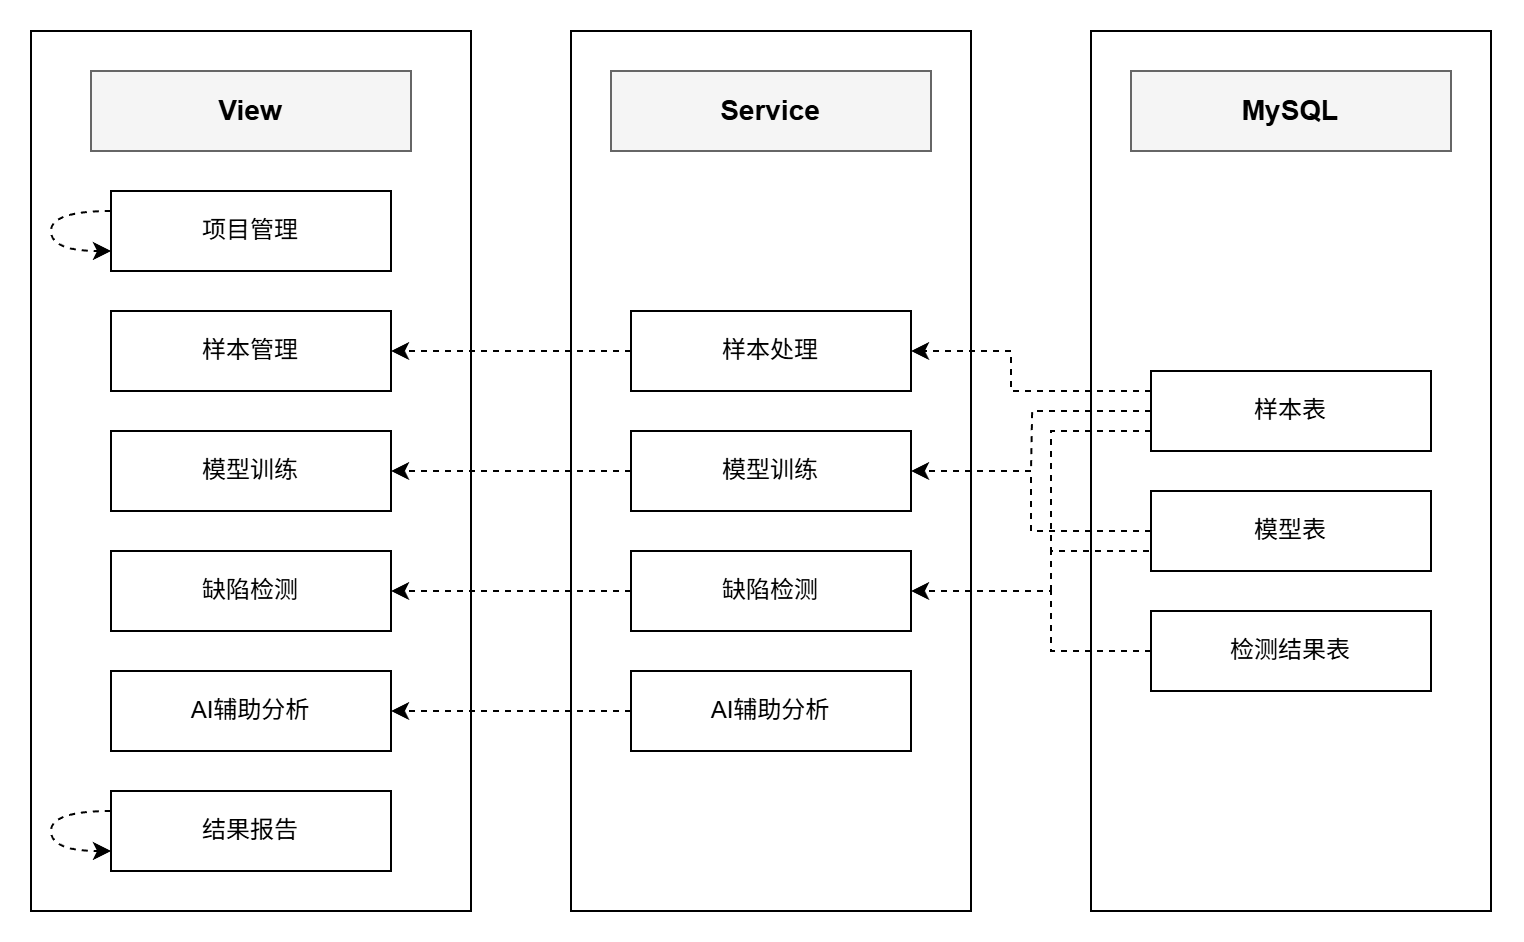
\includegraphics[width=\textwidth]{images/系统总体架构设计图.png}
    \caption{系统总体架构设计图}
    \label{系统总体架构设计图}
\end{figure}

\subsection{“4+1” 视图}

Kruchten 在 1995 年提出了软件体系结构的 “4+1” 的视图模型,如图 \ref{4+1视图} 所示。该模型从逻辑视图、过程视图、物理视图、开发视图和场景视图这五个不同的视角来描述软件体系结构。每一个视图针对系统的一个特定群体,专注于系统的一个侧面,五个视图描述了软件系统结构的全部内容\cite{[15]}。

\begin{figure}[htb]
    \centering
    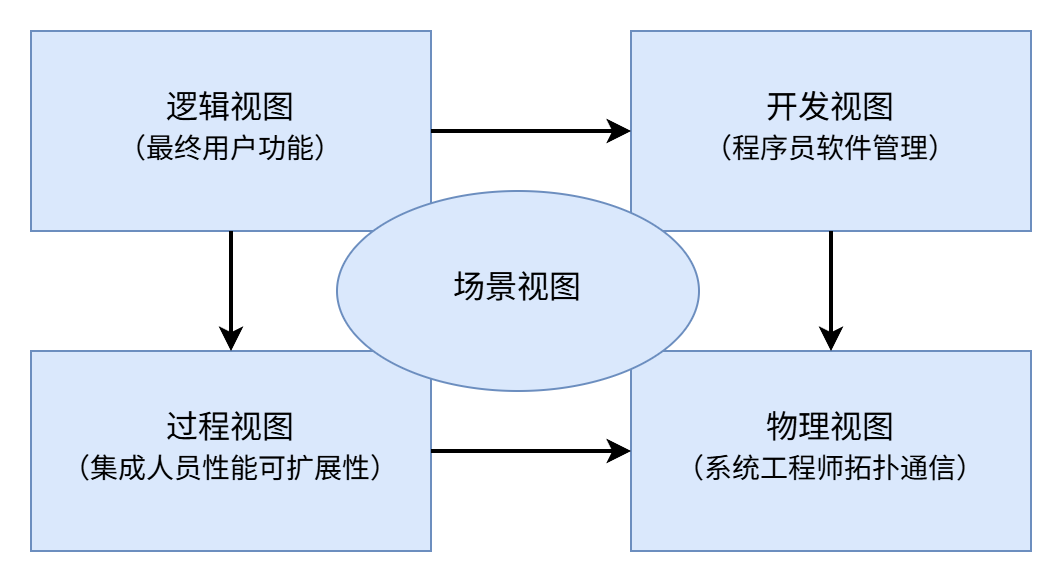
\includegraphics[width=0.6\textwidth]{images/4+1视图.png}
    \caption{“4+1” 视图}
    \label{4+1视图}
\end{figure}

(1)逻辑视图用于从结构化视角描述系统的功能需求,展示了对架构而言重要的元素和它们之间的关系,即系统为用户提供各项服务所具备的静态结构、组件关系和边界约束,反映了系统服务的构建过程。图 \ref{逻辑视图} 为系统逻辑视图。展示层根据用户行为与业务层进行交互,业务层通过数据层对相关数据进行操作并处理业务逻辑。

\begin{figure}[H]
    \centering
    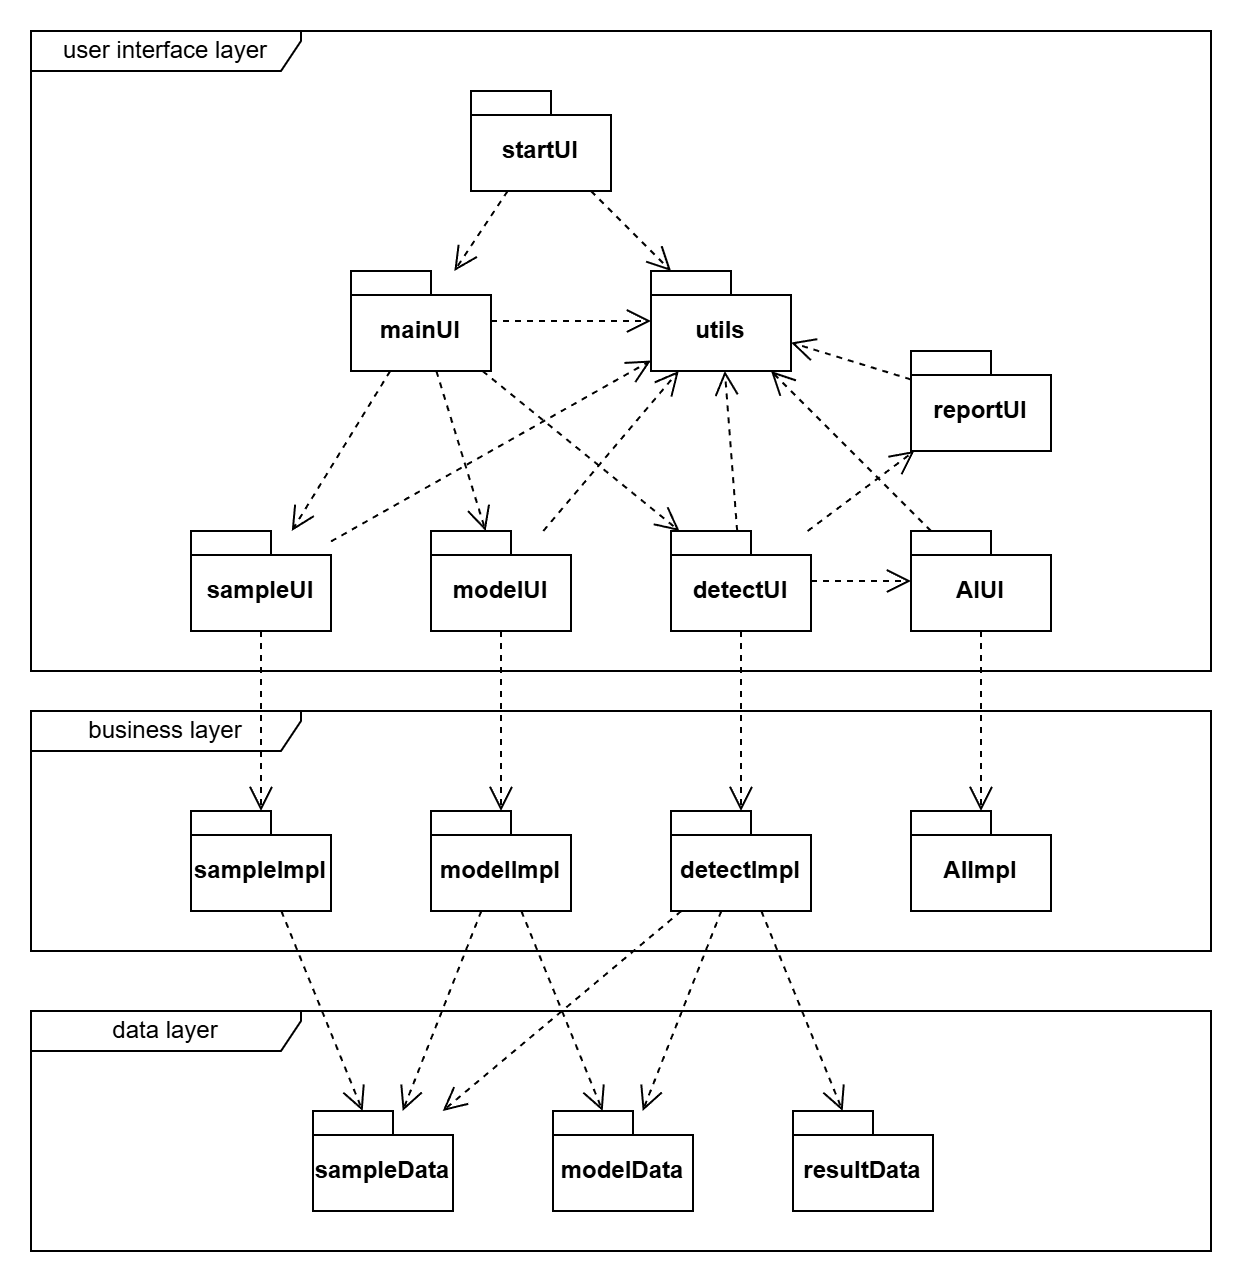
\includegraphics[width=0.8\textwidth]{images/逻辑视图.png}
    \caption{逻辑视图}
    \label{逻辑视图}
\end{figure}

(2)物理视图即部署视图,用于描述系统运行的物理环境或软件环境,前者包括移动终端、服务器等物理设备,后者包括虚拟机等,它们共同展示了系统的主要过程和组件是如何被映射到硬件上的。图 \ref{物理视图} 为系统物理视图。系统的客户端运行于移动终端上,而服务端以及数据库运行于服务器中。

\begin{figure}[H]
    \centering
    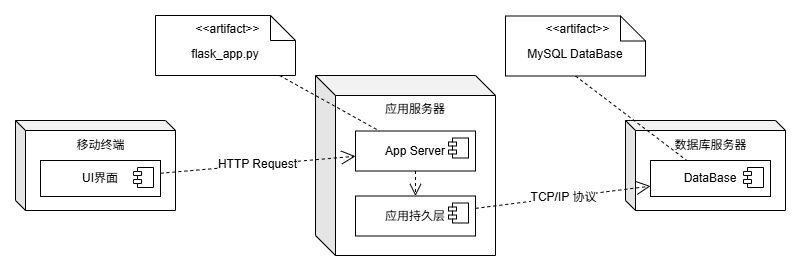
\includegraphics[width=\textwidth]{images/物理视图.png}
    \caption{物理视图}
    \label{物理视图}
\end{figure}

(3)过程视图即处理视图,用于描述系统的动态行为,即系统组件之间的通信、数据的输入输出,展示了元素之间的并发和交互。过程视图通常由 UML 的顺序图表示,图 \ref{过程视图} 为系统过程视图。

\begin{figure}[H]
    \centering
    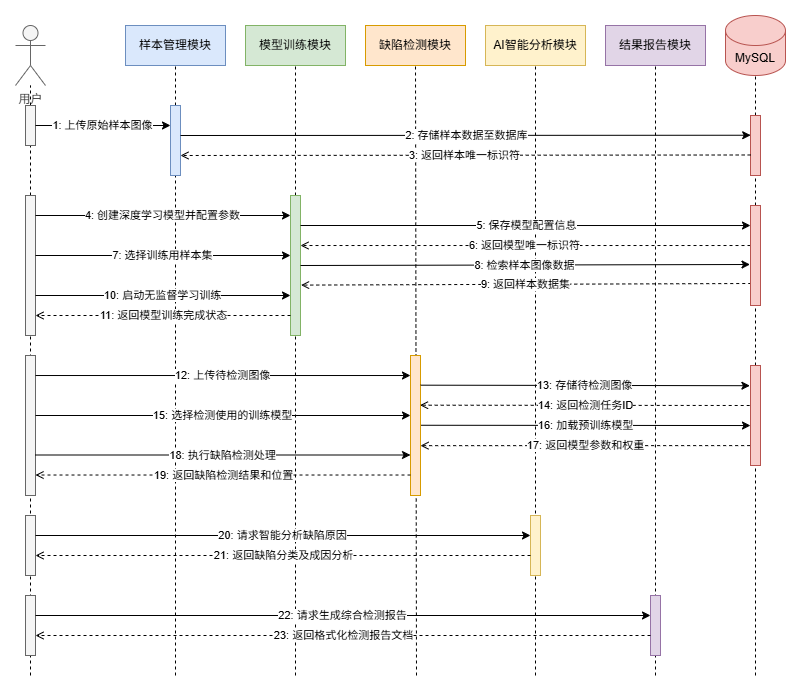
\includegraphics[width=\textwidth]{images/过程视图.png}
    \caption{过程视图}
    \label{过程视图}
\end{figure}

(4)开发视图用于描述软件模块的组织方式和开发管理策略,反映了软件组件的内部组织联系。图 \ref{开发视图} 为系统开发视图,展示了代码组织、构建流程、配置管理和依赖关系。

\begin{figure}[H]
    \centering
    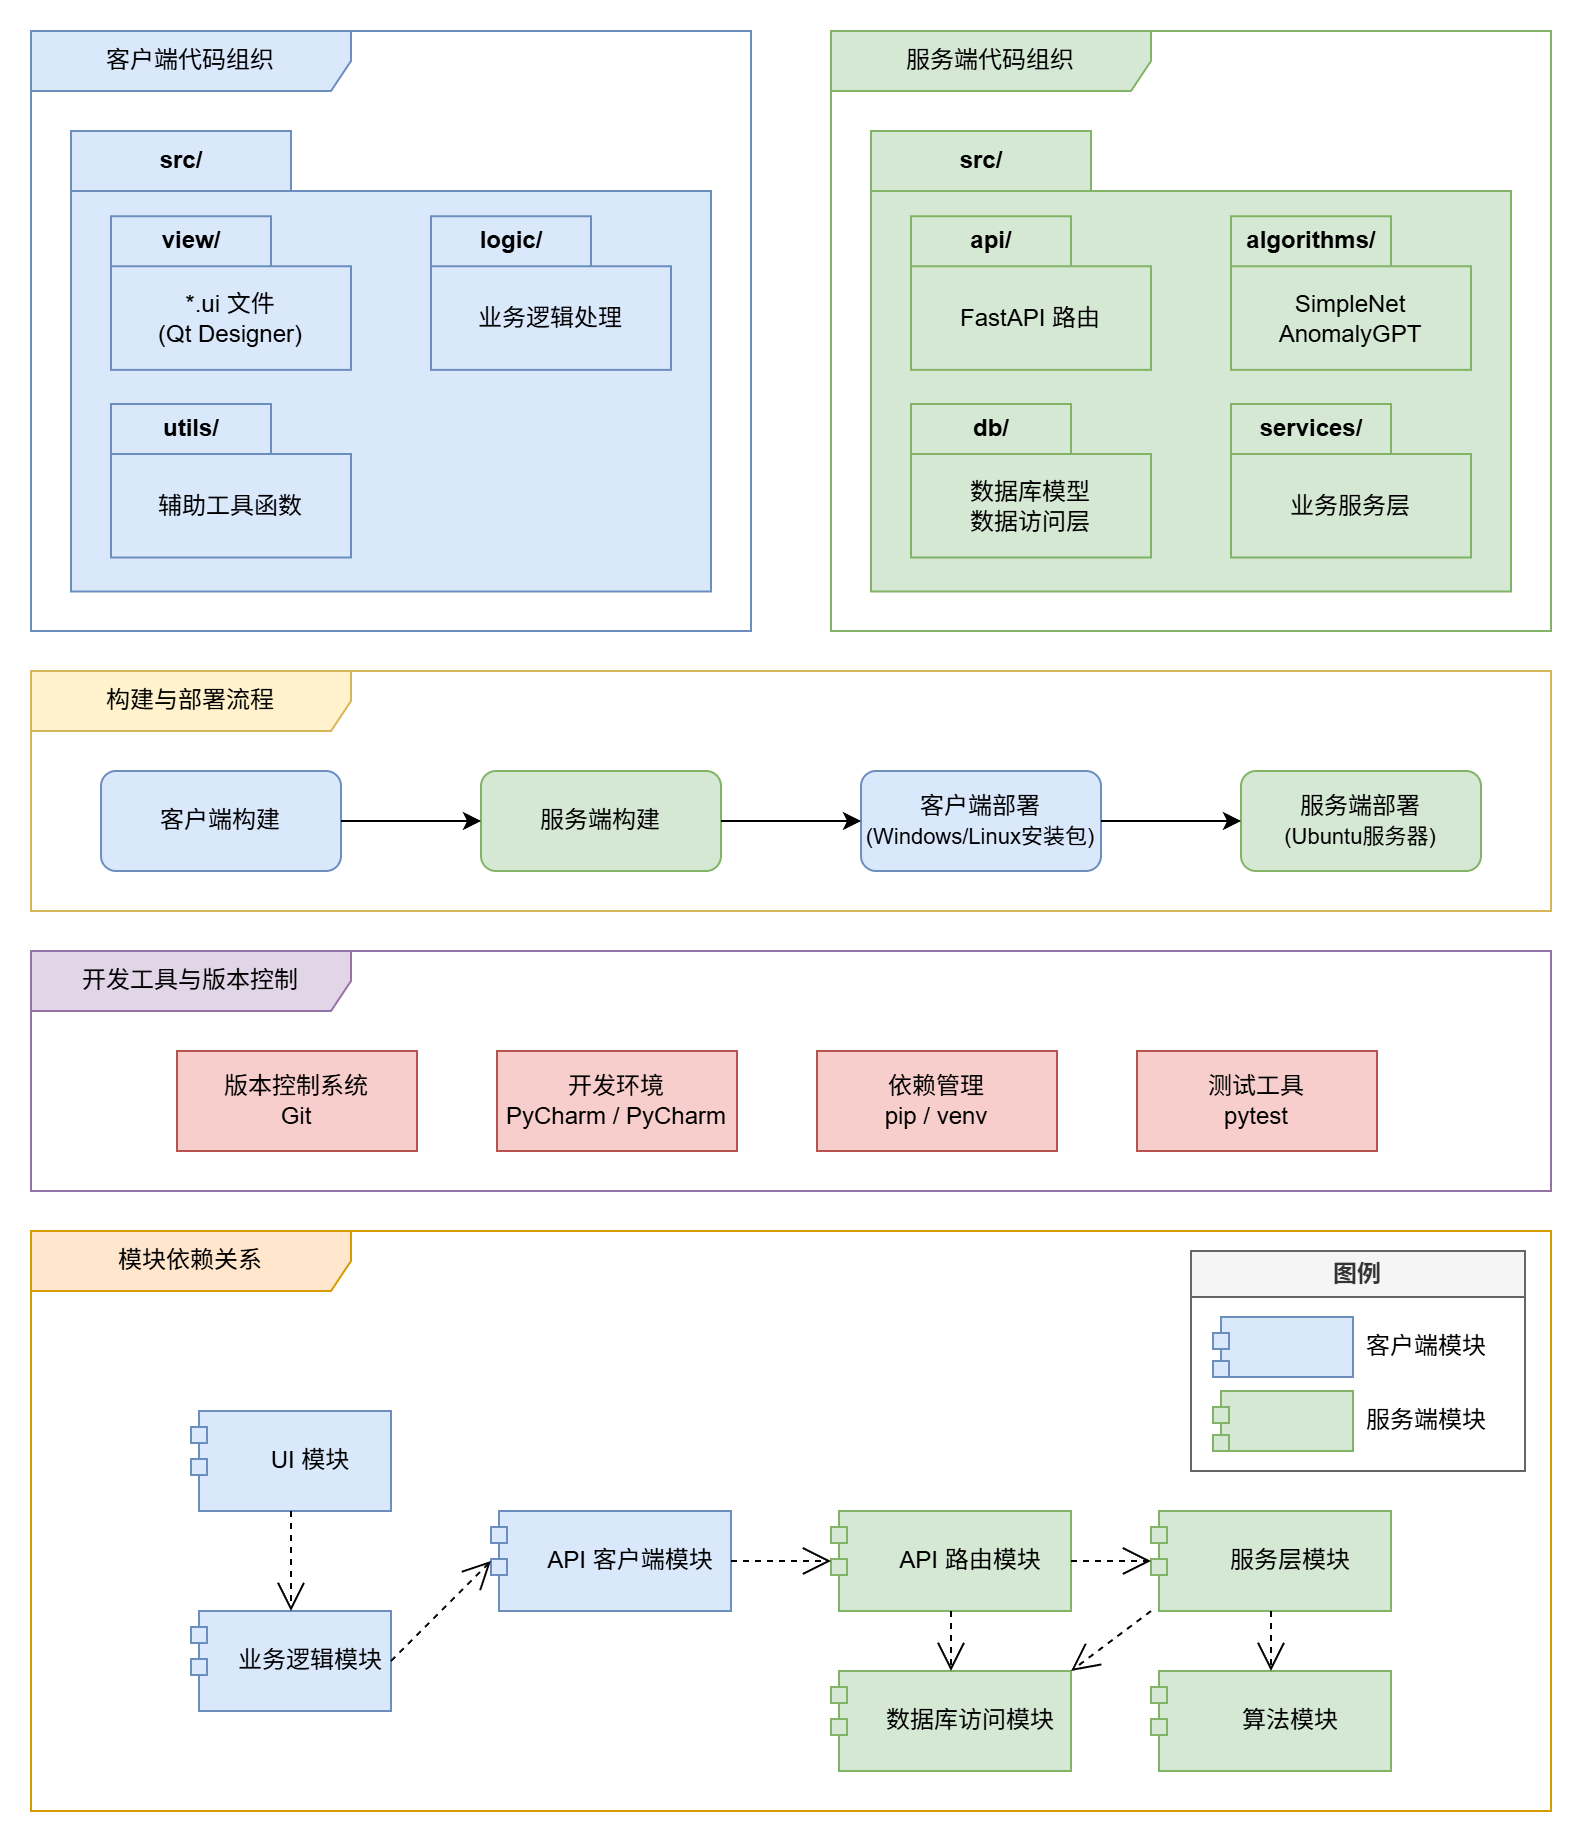
\includegraphics[width=0.8\textwidth]{images/开发视图.png}
    \caption{开发视图}
    \label{开发视图}
\end{figure}

(5)场景视图即用例图,用于描述参与者与用例间的关系,通过具体的用例场景,展示其他四个视图如何协同工作,反映系统的架构需求和交互设计。图 \ref{系统用例图} 为系统场景视图(用例图)。

\subsection{模块划分}

系统依据功能需求分为项目管理模块、样本管理模块、模型训练模块和缺陷检测模块四个主要功能模块,这四个模块又可以进一步划分为十一个子模块:项目信息模块、历史项目模块、计时器模块、样本组管理模块、样本处理模块、模型管理模块、训练模块、检测管理模块、检测模块、AI辅助分析模块、检测报告模块。
图 \ref{模块划分图} 为系统模块划分图。

\begin{figure}[htb]
    \centering
    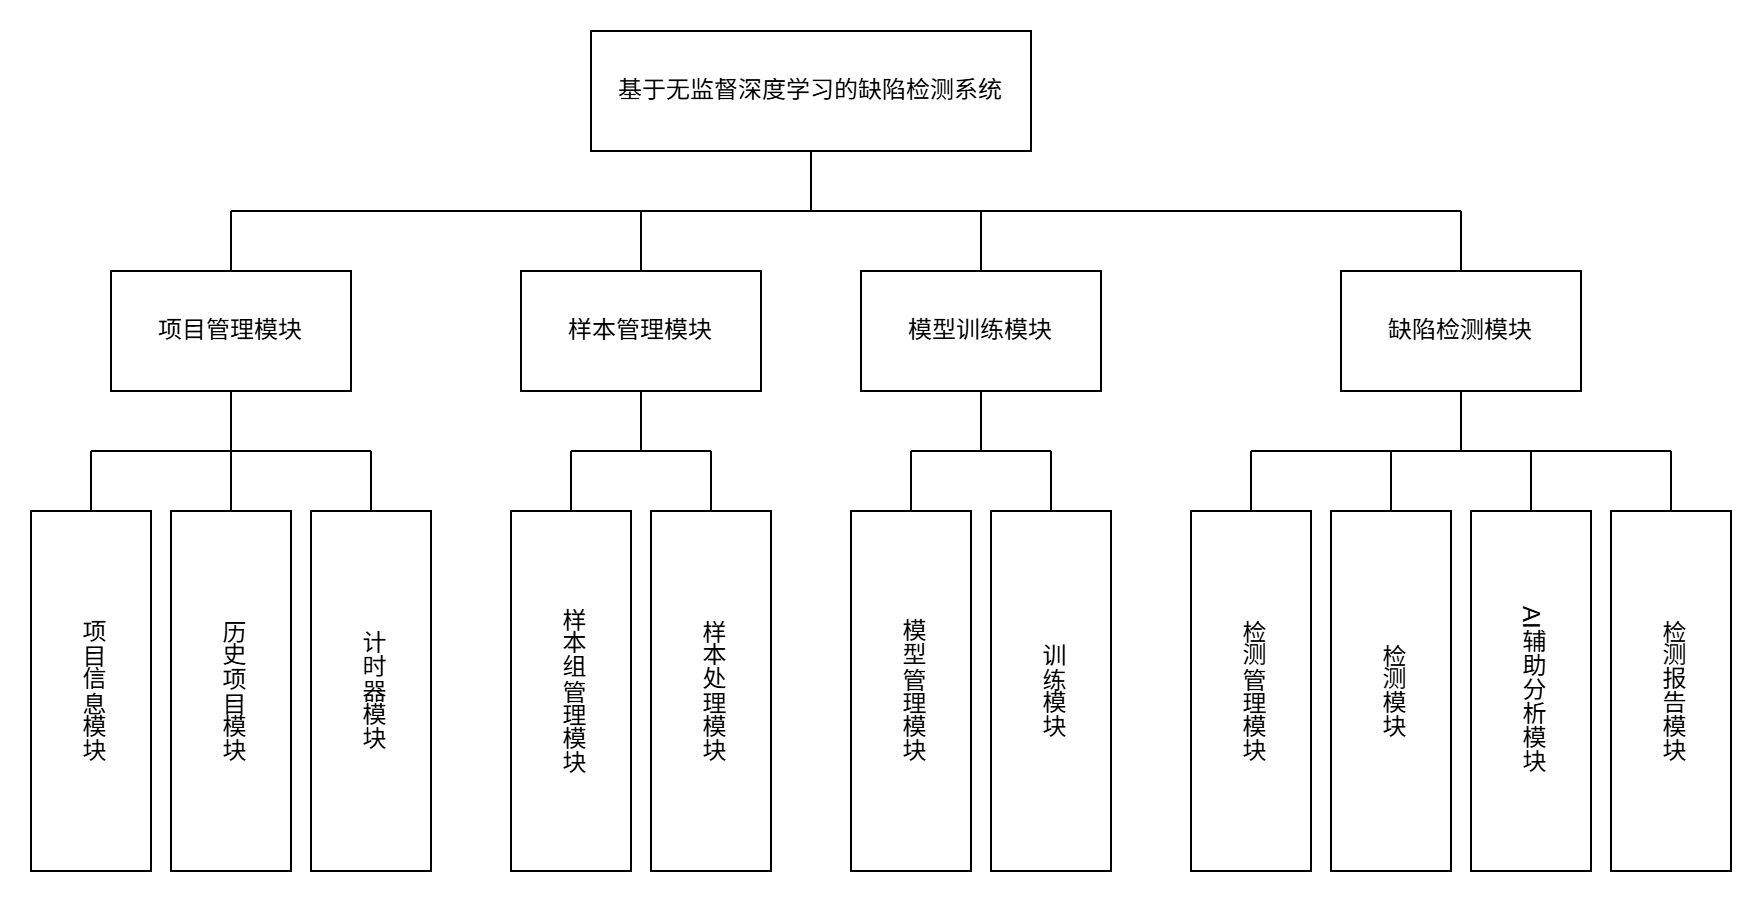
\includegraphics[width=\textwidth]{images/模块划分图.png}
    \caption{模块划分图}
    \label{模块划分图}
\end{figure}


\section{数据库设计}

\subsection{概述}

系统采用 MySQL 关系型数据库进行数据存储和管理。基于系统功能需求并结合数据特征,本课题设计了由样本表、样本组表、模型表、检测结果表,以及用于追踪模型训练和推理过程的模型训练样本关联表和模型推理样本关联表这六个表组成的数据库结构。数据库的设计遵循实用性和高效性原则,综合考虑数据的完整性和查询效率。

\subsection{E-R图设计}

\begin{figure}[H]
    \centering
    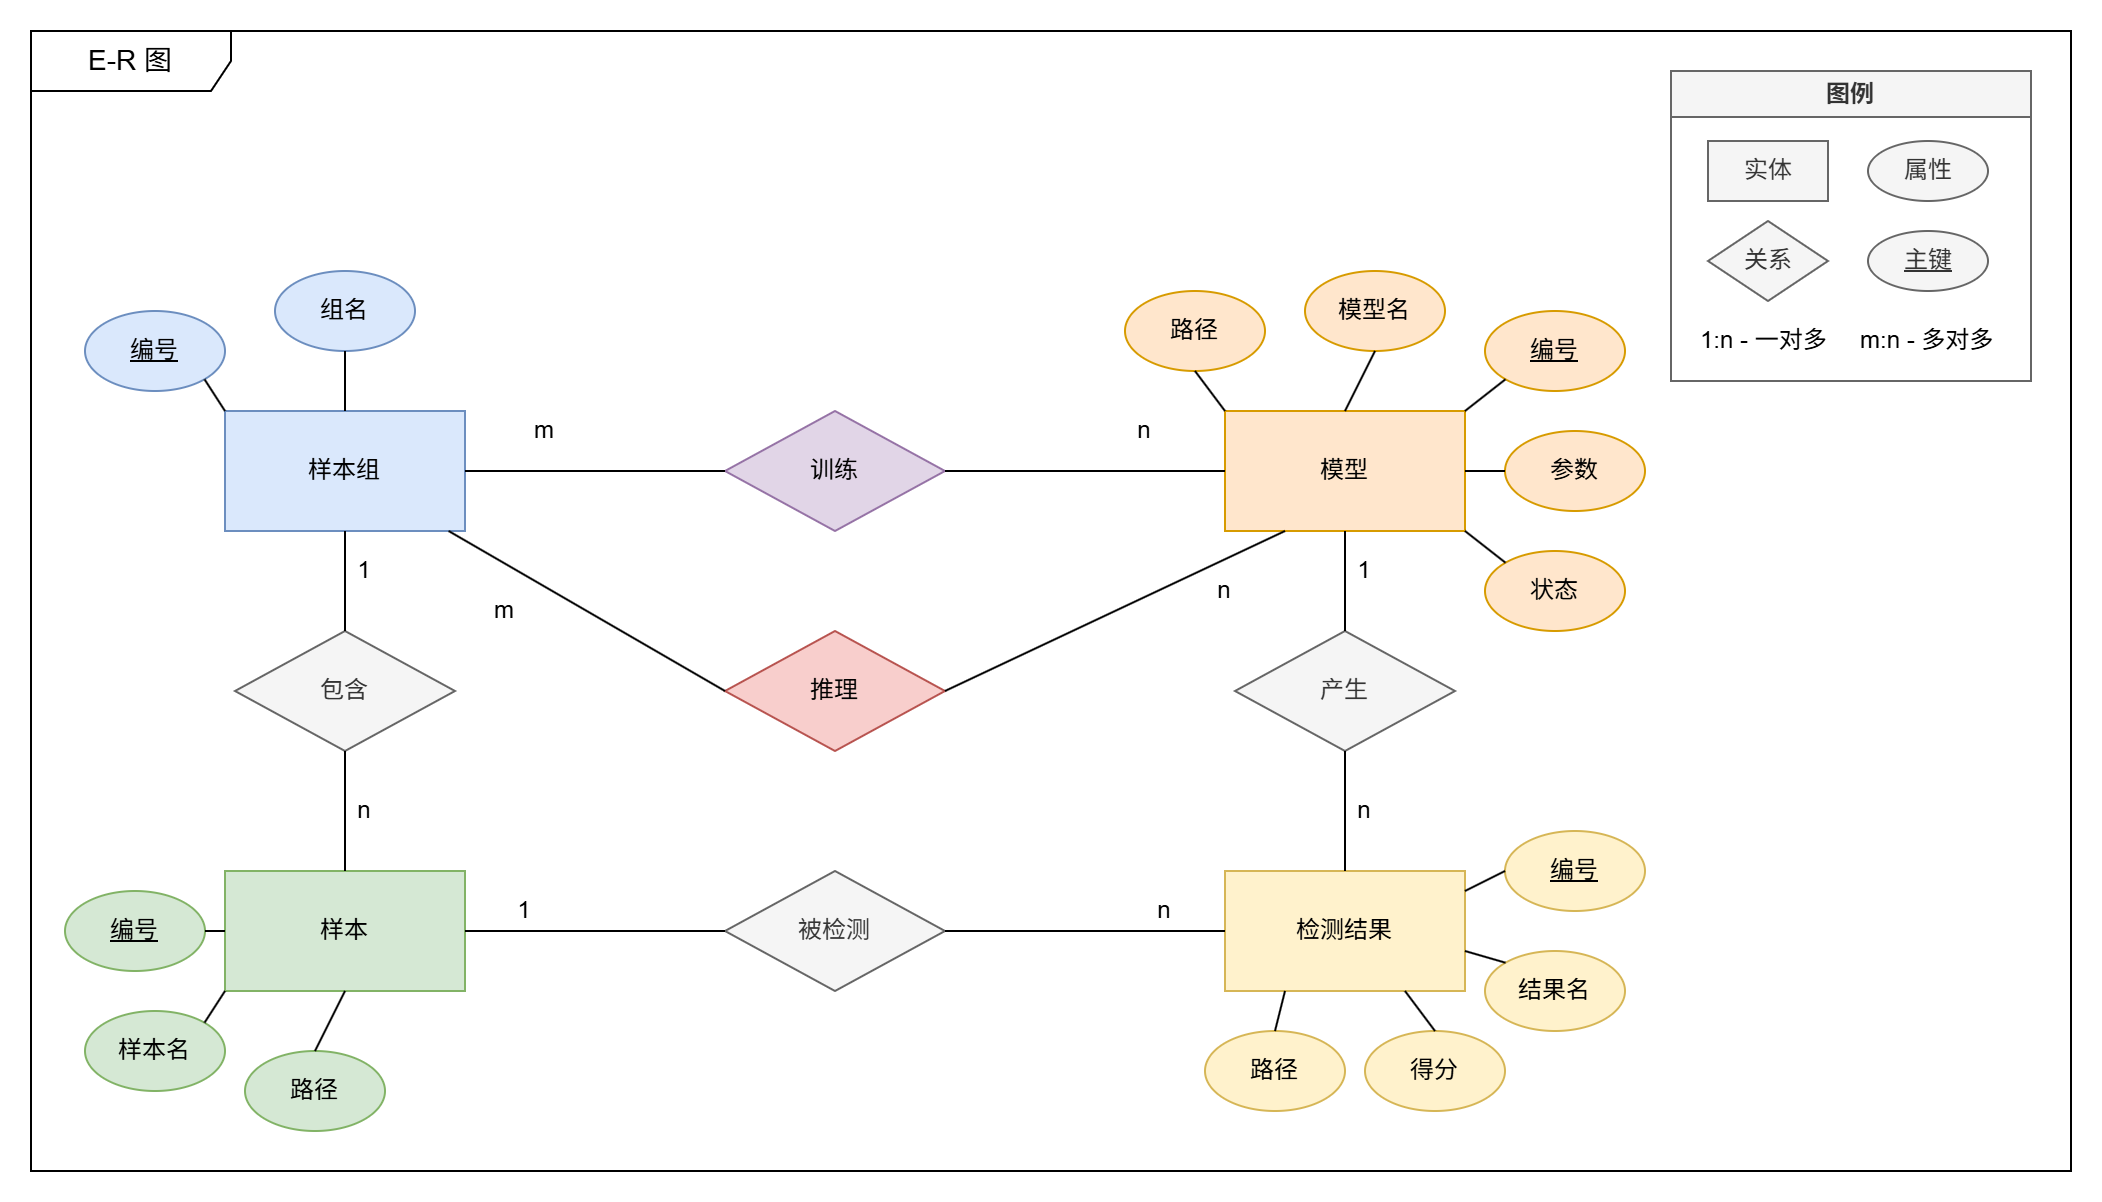
\includegraphics[width=\textwidth]{images/E-R图.png}
    \caption{E-R图}
    \label{E-R图}
\end{figure}

系统的实体关系图如图 \ref{E-R图} 所示。其中,系统的实体包括:样本组,用于存储样本集合的基本信息;样本,记录单个样本图像的详细信息;模型,存储训练好的模型及其参数;检测结果,记录缺陷检测的结果数据。实体间的关系包括:一个样本组包含多个样本;检测结果关联到特定的样本和使用的模型;模型与训练样本之间存在多对多关系;模型与推理样本之间存在多对多关系。

\subsection{核心表结构}

(1)样本组表 (sample\_group) 如图 \ref{样本组表} 所示。

\begin{figure}[H]
    \begin{lstlisting}[language=sql]
sample_group(
  id INT PRIMARY KEY AUTO_INCREMENT,  // 样本组ID,主键
  name VARCHAR(100) NOT NULL          // 样本组名称
)
    \end{lstlisting}
    \caption{样本组表}
    \label{样本组表}
\end{figure}

(2)样本表(sample) 如图 \ref{样本表} 所示。

\begin{figure}[H]
    \begin{lstlisting}[language=sql]
sample(
  id INT PRIMARY KEY AUTO_INCREMENT,  // 样本ID,主键
  name VARCHAR(100) NOT NULL,         // 样本名称
  group_id INT NOT NULL,              // 所属样本组ID,外键
  path VARCHAR(255) NOT NULL,         // 样本课题件路径
  FOREIGN KEY (group_id) REFERENCES sample_group(id)
)
    \end{lstlisting}
    \caption{样本表}
    \label{样本表}
\end{figure}

(3)模型表(model) 如图 \ref{模型表} 所示。

\begin{figure}[H]
    \begin{lstlisting}[language=sql]
model(
  id INT PRIMARY KEY AUTO_INCREMENT,                  // 模型ID,主键
  name VARCHAR(100) NOT NULL,                         // 模型名称
  path VARCHAR(255) NOT NULL,                         // 模型文件路径
  input_h INT NOT NULL,                               // 输入高度  
  input_w INT NOT NULL,                               // 输入宽度
  end_acc FLOAT NOT NULL,                             // 结束精度
  layers INT NOT NULL,                                // 使用的层数
  patchsize INT NOT NULL,                             // 补丁大小
  embed_dimension INT NOT NULL,                       // 嵌入维度
  status ENUM('NEW','TRAINING','READY','INFERRING'),  // 模型状态
)
    \end{lstlisting}
    \caption{模型表}
    \label{模型表}
\end{figure}

(4)检测结果表(detection\_result) 如图 \ref{检测结果表} 所示。

\begin{figure}[H]
    \begin{lstlisting}[language=sql]
detection_result(
  id INT PRIMARY KEY AUTO_INCREMENT,  // 结果ID,主键
  name VARCHAR(100) NOT NULL,         // 结果名称
  sample_id INT NOT NULL,             // 检测的样本ID,外键
  model_id INT NOT NULL,              // 检测的模型ID,外键
  score FLOAT NOT NULL,               // 异常分数
  path VARCHAR(255) NOT NULL,         // 检测结果文件路径
  FOREIGN KEY (sample_id) REFERENCES sample(id),
  FOREIGN KEY (model_id) REFERENCES model(id)
)
    \end{lstlisting}
    \caption{检测结果表}
    \label{检测结果表}
\end{figure}

(5)模型训练样本表(model\_trained\_sample) 如图 \ref{模型训练样本表} 所示。

\begin{figure}[H]
    \begin{lstlisting}[language=sql]
model_training_sample(
  id INT PRIMARY KEY AUTO_INCREMENT,  // 关联ID,主键
  model_id INT NOT NULL,              // 模型ID,外键
  sample_id INT NOT NULL,             // 样本ID,外键
  FOREIGN KEY (model_id) REFERENCES model(model_id),
  FOREIGN KEY (sample_id) REFERENCES sample(sample_id),
  UNIQUE KEY (model_id, sample_id)    // 确保一个样本在一个模型中只被训练一次
)
    \end{lstlisting}
    \caption{模型训练样本表}
    \label{模型训练样本表}
\end{figure}

(6)模型推理样本表(model\_inferred\_sample) 如图 \ref{模型推理样本表} 所示。

\begin{figure}[H]
    \begin{lstlisting}[language=sql]
model_inference_sample(
  id INT PRIMARY KEY AUTO_INCREMENT,  // 关联ID,主键
  model_id INT NOT NULL,              // 模型ID,外键
  sample_id INT NOT NULL,             // 样本ID,外键
  score FLOAT NOT NULL,               // 异常分数
  FOREIGN KEY (model_id) REFERENCES model(model_id),
  FOREIGN KEY (sample_id) REFERENCES sample(sample_id),
  UNIQUE KEY (model_id, sample_id)    // 确保一个样本在一个模型中只被记录一次
)
    \end{lstlisting}
    \caption{模型推理样本表}
    \label{模型推理样本表}
\end{figure}

\subsection{数据关系与完整性}

系统采用外键约束维护表间关系,确保数据的引用完整性:样本表引用 group\_id,关联到样本组表;检测结果表、模型训练样本关联表、模型推理样本关联表均引用 sample\_id 和 model\_id,关联到模型表和样本表

数据库操作采用适当的级联规则,例如:删除样本组时,关联的样本记录自动删除;删除模型时,相关的检测结果仍然保留以便历史查询。

通过这种简洁而功能完备的数据库结构,系统能够有效支持样本管理、模型训练和缺陷检测结果存储,为用户提供完整的数据支持。

\section{本章小结}

本章对缺陷检测系统进行了全面的分析与设计,从实际工业场景出发,首先明确了系统作为工业质检辅助工具的目标,再借助用例详细分析了系统的功能需求和非功能需求,然后通过 “4+1” 视图模型从多个视角描述了软件体系结构,接着将系统划分为四个主要功能模块和十一个子模块,最后设计了数据库结构作为系统的数据支撑。

\chapter{系统实现}

\section{开发环境}

客户端运行于 Windows 11 64 位操作系统上,在 Python 3.11 和 PySide6 环境下开发,客户端部署在 Ubuntu 22.04 服务器上,采用 Git 进行版本控制。

\section{核心模块实现}

\subsection{项目管理模块}

项目管理模块是整个缺陷检测系统的基石,主要负责项目的创建、加载和运行,以及项目信息的管理,为整个缺陷检测系统提供项目层面的数据支持。

(1)项目信息模块

项目信息模块是项目管理中的核心,负责项目的创建以及基本信息的存取和管理,为整个缺陷检测系统提供项目层面的数据支持。如图 \ref{开始界面} 所示,用户点击新建按钮创建项目,然后在后续操作中不断完善项目信息;用户点击打开按钮或直接将项目文件夹拖入窗口即可打开已有项目,便于用户继续上一次未完成的工作,或对已完成的工作进行调整后重新处理。

\begin{figure}[htb]
    \centering
    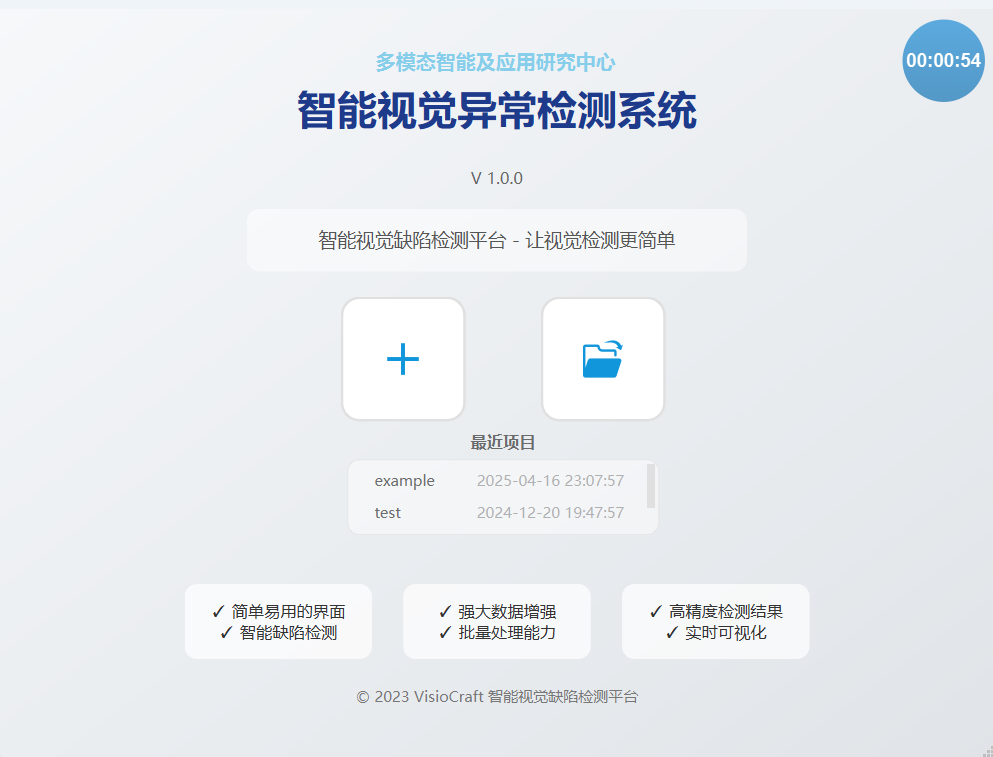
\includegraphics[width=\textwidth]{images/开始界面.png}
    \caption{开始界面}
    \label{开始界面}
\end{figure}

项目信息包括项目元数据,如项目名称、项目路径、模型组、训练样本组、检测样本组等的存取,以及项目相关目录和配置信息。项目结构如图 \ref{项目结构图} 所示,整个项目包含项目元数据文件,以及样本组、模型组、检测组三个文件夹,每个文件夹中包含多个子文件夹,里面存放了具体样本组、模型组、检测组的相关信息。其中,项目元数据文件 metadata.json 在新建项目时自动生成,并在后续用户操作中不断更新。而样本列表信息 sample\_list.json、模型配置信息 model.json、检测结果列表 detect\_list.json 等依次在样本管理、模型训练与缺陷检测过程中被创建或修改。

\begin{figure}[htb]
    \centering
    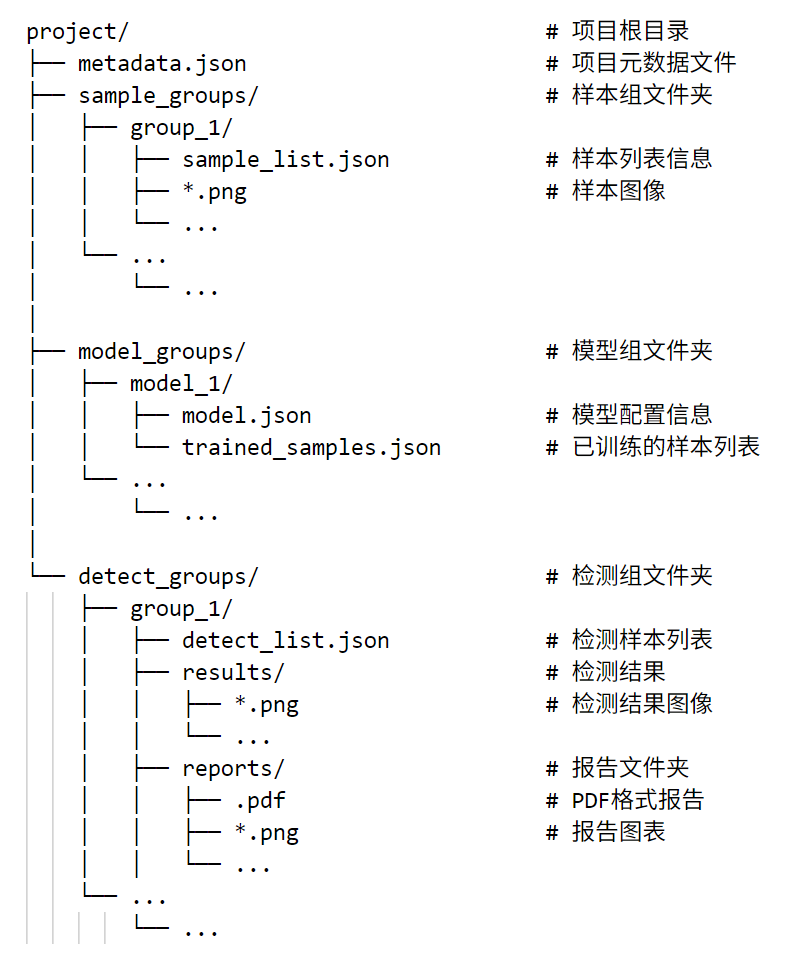
\includegraphics[width=0.6\textwidth]{images/项目结构图.png}
    \caption{项目结构图}
    \label{项目结构图}
\end{figure}

(2)历史项目模块

历史项目模块主要负责记录、管理和快速访问用户最近操作过的项目。历史项目列表存储在本地文件中,用户新访问的项目会自动添加到列表开头,实现按时间排序;当项目已在列表中时,会先移除旧记录再添加到列表首位。历史项目列表栏详见图 \ref{开始界面},双击列表项即可打开对应项目,若项目路径不存在,自动从列表中移除并提示用户。

(3)计时器模块

计时器是项目中的辅助组件,负责追踪项目的运行时间,帮助用户记录和评估工作时长。该模块使用 utils 包中的 FloatingTimer 类实现,覆盖整个应用程序的生命周期。

如图 \ref{开始界面} 所示,计时器模块以悬浮球的形式显示,默认位于主窗口右上角,不影响主界面操作,用户也可以拖拽悬浮球到任意位置。悬浮球上显示了当前项目操作的时间,用户可以双击悬浮球来重置计时器,便于分段计时。计时器通过窗口位置监控机制实现了拖拽功能,以及在各界面无缝切换,保证了在整个应用使用过程中时间记录的连续性。

\subsection{样本管理模块}

样本管理模块是缺陷检测系统的基础组件,负责样本的组织、存储和预处理,为后续的模型训练和缺陷检测提供高质量的数据支持。

(1)样本组管理模块

样本组管理模块是样本管理的基础,负责组织和管理样本集合及其状态。如图 \ref{样本界面} 所示,用户可以创建、导入、删除样本组,或上传样本组到服务器。其中导入和删除样本组的管理界面详见图 \ref{样本组列表},界面列出了目前系统所创建的所有样本组的名称及其状态。新建或导入样本组后,系统会将其元数据记录下来,并在下次打开项目时自动加载。样本组所包含的样本由样本列表栏显示,列表栏支持从本地文件夹中批量导入样本图像,以及选择单个或多个样本文件进行添加。在列表栏点击导入的样本可进行查看与编辑,点击选择按钮可多选或删除样本。当用户新建、切换或删除样本组后,系统会刷新样本列表栏,并修改样本组的状态。样本组的状态控制着样本列表操作按钮的显示与否,仅当样本组存在时用户才能对样本进行导入、删除等操作。样本编辑完成后,用户可以将样本组上传到服务器中,以备后续使用。系统会跟踪上传进度,为用户提供动态反馈。另外,在用户进入模型训练流程之前,系统会自动判断样本组是否上传至服务器,以防用户遗忘。只有样本组上传完成后,用户才能进行下一步操作。

\begin{figure}[htb]
    \centering
    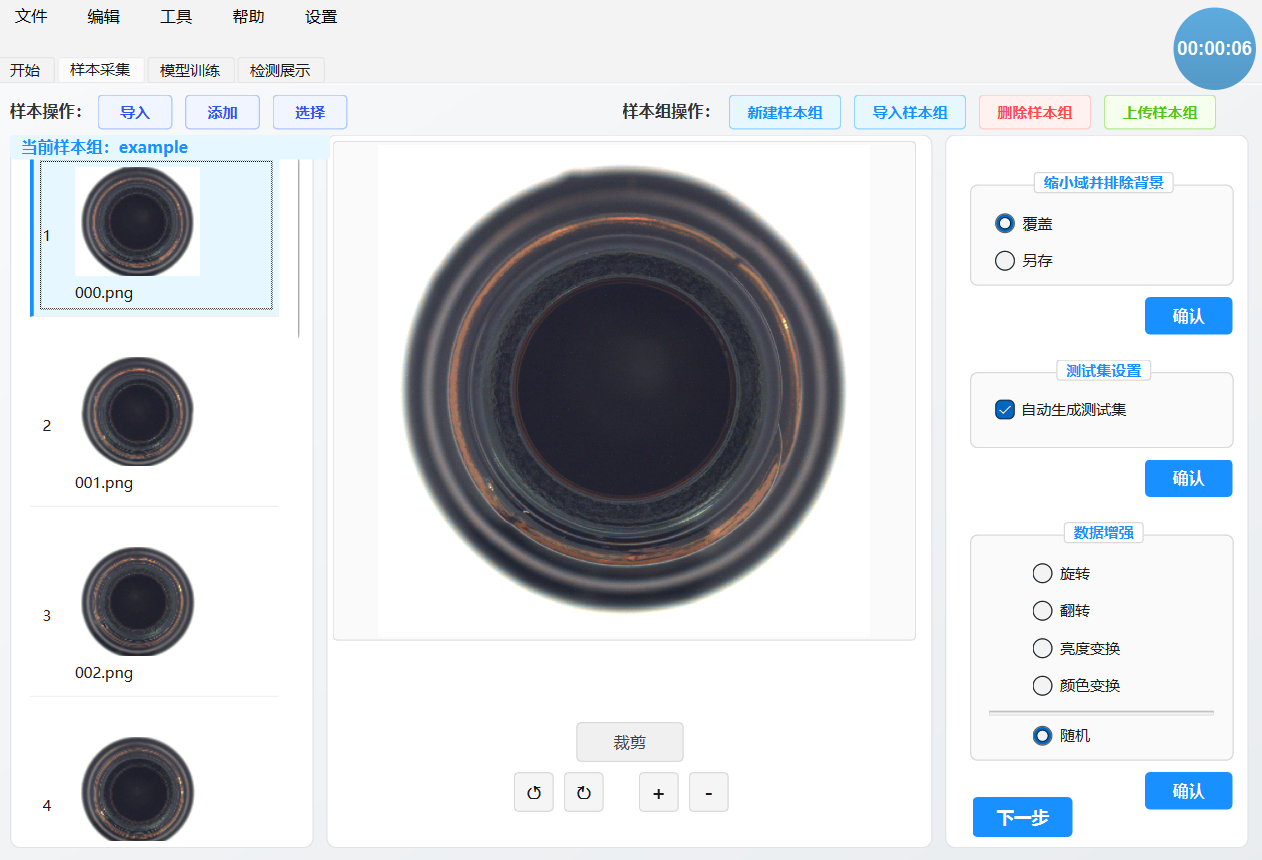
\includegraphics[width=\textwidth]{images/样本界面.png}
    \caption{样本界面}
    \label{样本界面}
\end{figure}

\begin{figure}[htb]
    \centering
    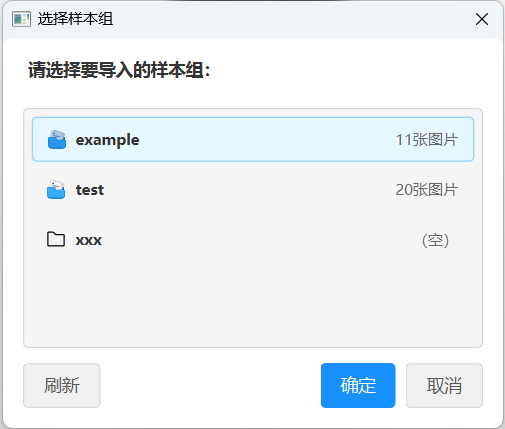
\includegraphics[width=0.5\textwidth]{images/样本组列表.png}
    \caption{样本组列表}
    \label{样本组列表}
\end{figure}

(2)样本处理模块

样本处理模块是样本管理的核心部分,它负责单个或多个样本的预处理工作,如裁剪、背景排除和数据增强。裁剪和背景排除的目的相同,都是为了去除不必要的图像部分,减少背景干扰,从而突出检测的目标区域,提高检测的准确率;数据增强可以增强样本的多样性,提高模型的泛化能力。

排除背景缩小域的功能通过分割算法识别并保留图像的主体部分,保证后续的数据增强以及模型训练集中于图像的目标区域,适用于背景相对明显的样本。相较于手动裁剪,它可以对样本进行批量处理,效率更高。该功能使用 OpenCV 库实现,先对图像进行阈值处理、轮廓检测和过滤,然后基于形态学操作进行轮廓优化,去除噪点和细小碎片。具体来说,就是先把图像灰度化并进行二值化处理,以分离前景和背景,然后进行轮廓检测和筛选,保留主要目标区域,最后计算目标区域的最小外接矩形,自动裁剪图像。同时,为确保目标的完整性,避免过度裁剪,系统计算外接矩形时会主动添加适当边距。

数据增强功能可对图像进行多种变换,从而扩充训练样本集,增强模型的泛化能力,适用于样本数量较少的情况。数据增强支持批量处理,使用 OpenCV 库对选中的样本进行几何变换和外观变换,包括旋转、翻转、亮度变化和颜色变换。用户既能选择特定方式,也可以选择随机变换对样本进行数据增强。变换后的图像会自动显示于样本列表栏中,并被保存到当前样本组文件夹。另外,由于无监督学习模型的训练集要求是正向样本,数据增强功能只会对样本进行轻微调整。

图像裁剪功能使用户能够通过交互式裁剪框手动去除样本中无关区域,可以进一步优化背景排除的效果,适用于背景排除算法效果不佳且样本量较少的情况。基于自定义的 ResizableRectItem 类实现可调整大小的裁剪框,在 QGraphicsView 中通过 QGraphicsScene 构建互动场景,实现矩形的拖拽和缩放。用户点击裁剪按钮后,裁剪框会自动显示在图像上,用户将鼠标移至裁剪框的边界点时,会自动切换光标样式,此时可拖拽边框来调整裁剪区域的大小。缩放或移动矩形区域后,裁剪框以外的图像部分会自动变模糊,反差对比明显。点击接受按钮,裁剪框自动消失,且裁剪区域以外的部分被丢弃。此时,用户可选择保存裁剪图像,样本列表栏中图像的预览图以及中央的大图会自动刷新并自适应。在以上过程中,用户可以随时点击取消按钮,取消裁剪操作,此时裁剪框会自动消失,图像恢复原状。另外,系统在裁剪时会临时禁用其它编辑功能,以防用户误操作。

ResizableRectItem 类是仿照安卓手机的相片编辑功能对 Qt 的 QGraphicsRectItem 进行改造的,实现了可调整大小的矩形裁剪框,支持拖拽、缩放等操作。它使用悬停反馈机制,监控鼠标位置,当鼠标处于裁剪框边缘时自动切换光标样式;重写鼠标按压、移动、释放事件,实现裁剪框的拖拽、缩放等操作。裁剪时,矩形以外的区域会自动模糊,如图 \ref{裁剪画面} 所示,增强了用户对选定区域的感知,另外,系统会临时禁用界面上的其它图像编辑组件,确保操作的一致性。

\begin{figure}[htb]
    \centering
    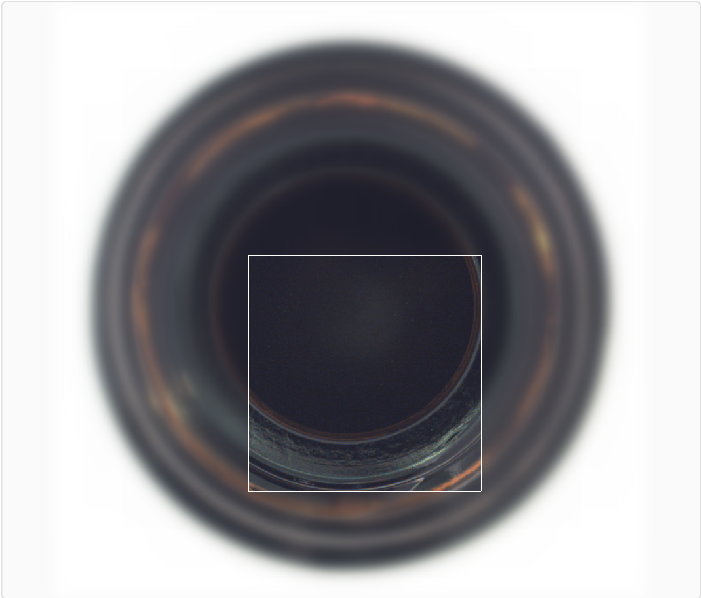
\includegraphics[width=0.3\textwidth]{images/裁剪画面.png}
    \caption{裁剪画面}
    \label{裁剪画面}
\end{figure}

\subsection{模型训练模块}

模型训练模块是应用基于无监督深度学习的缺陷检测算法的核心组件,负责管理和训练缺陷检测模型。

(1)模型管理模块

模型管理模块是模型训练的准备工作,负责组织和管理模型及其配置信息。如图 \ref{模型界面} 所示,用户可以创建、导入、删除模型,以及调整模型参数,其中导入和删除的管理界面与样本管理模块类似,唯一的区别就是用灰色、黄色和绿色分别标识了未训练、训练或推理中、已训练这几种状态,此处不再赘述。当用户新建或导入模型后,可进行参数设置,系统提供了参数映射功能,通过模型精度、缺陷大小、训练速度三个选项的配置可自动生成模型参数建议值,为新手或想要快速完成训练过程的用户给予方便。该机制首先从精度维度确定特征提取深度和嵌入维度,再从缺陷大小维度设定输入分辨率和补丁大小,最后通过训练速度维度对参数进行整体微调,实现参数间的协同配置。当然,专业用户也可以在详细编辑界面进行手动设置,如图 \ref{参数设置} 所示,系统暂时只支持配置输入尺寸、结束精度、补丁大小、特征层、嵌入维度这几个参数。参数设置完成后,模型相关信息会被自动同步到服务器,同时保存到本地,以便后续使用。

\begin{figure}[H]
    \centering
    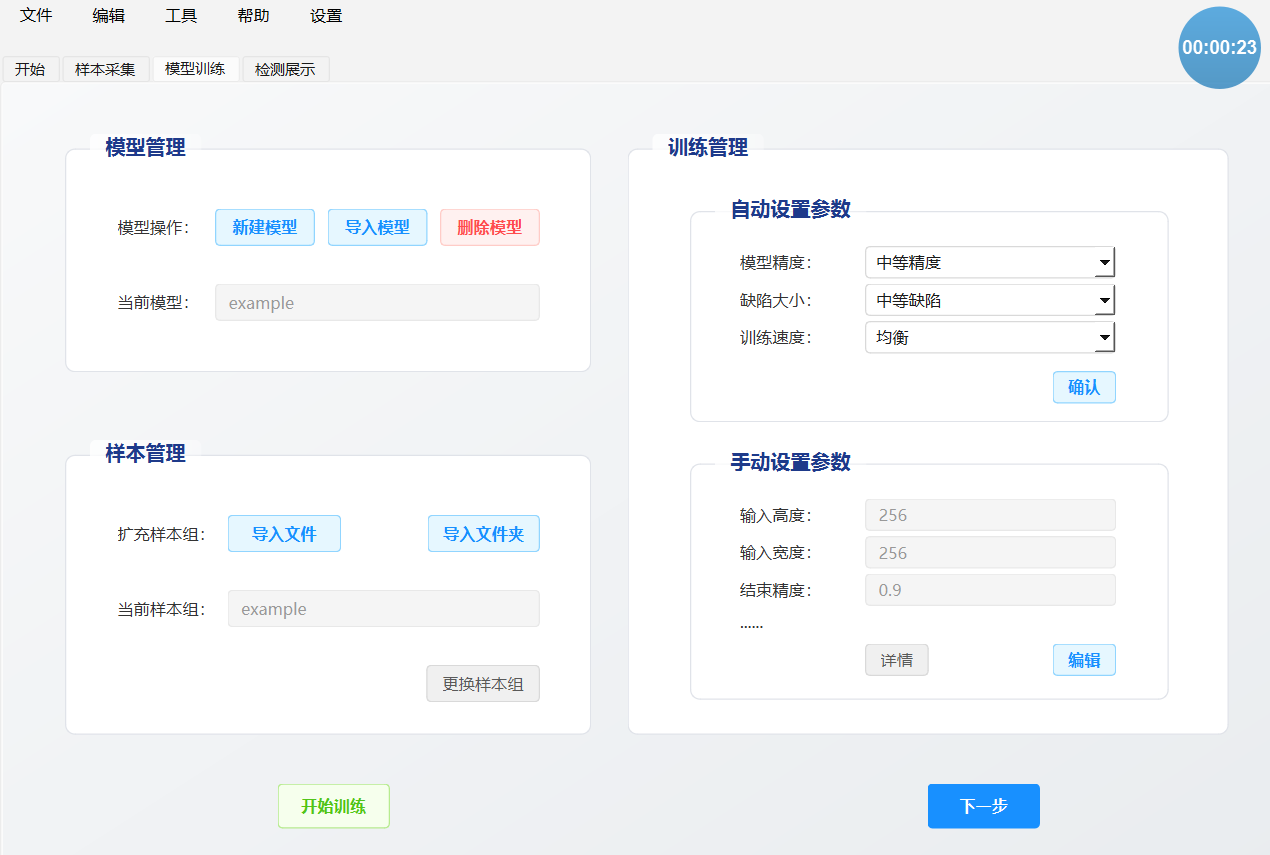
\includegraphics[width=\textwidth]{images/模型界面.png}
    \caption{模型界面}
    \label{模型界面}
\end{figure}

\begin{figure}[htb]
    \centering
    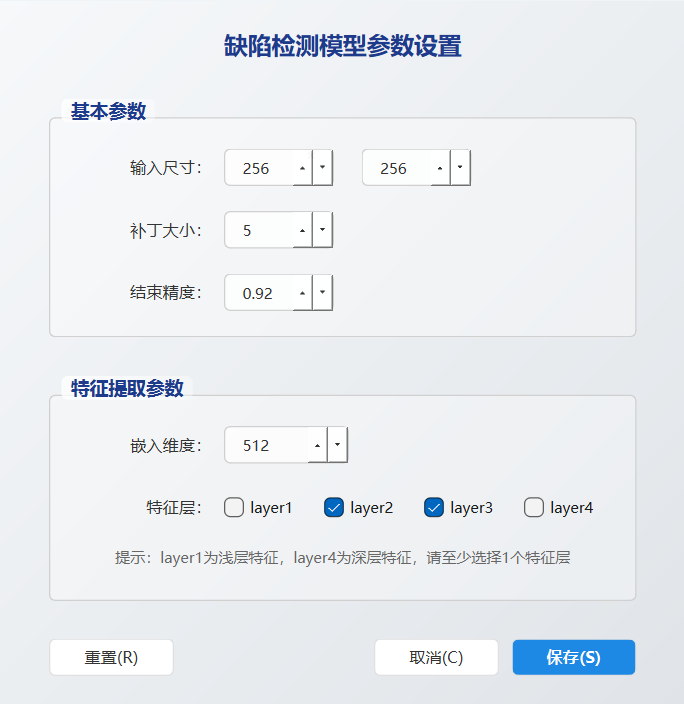
\includegraphics[width=0.5\textwidth]{images/参数设置.png}
    \caption{参数设置}
    \label{参数设置}
\end{figure}

(2)训练模块

训练模块负责模型的实际训练过程,具体包括训练执行、训练进度可视化以及模型状态控制等部分。训练前系统会自动判断样本组和模型组的有效性,比如样本组是否为空、模型是否处于未训练状态等。启动训练后,系统进入等待态,界面显示加载动画,直至获取到第一轮训练的结果。此时开始显示训练的实时进度,如图 \ref{训练进度} 所示,界面展示了动态概率曲线,以及当前训练轮次、训练时间、训练精度等指标。其中,训练曲线的可视化组件在 Qt 图表框架的基础上构建。系统定时从后台拉取训练数据来实时更新图表,并通过 QChart 和 QLineSeries 在坐标轴上实现动态绘制。训练曲线组件支持全局视图与局部放大图这两种视角的切换,使用户可以灵活地观察训练的整体趋势与细节变化。另外,如果用户在训练过程中急需使用模型,可以随时点击结束按钮终止训练。当模型达到目标精度或用户手动终止训练以后,训练结束,模型自动恢复空闲状态。同样地,在用户进入缺陷检测流程前,系统会自动检查模型是否被训练并给出提醒,在训练结束后用户才能继续下一步操作。

\begin{figure}[htb]
    \centering
    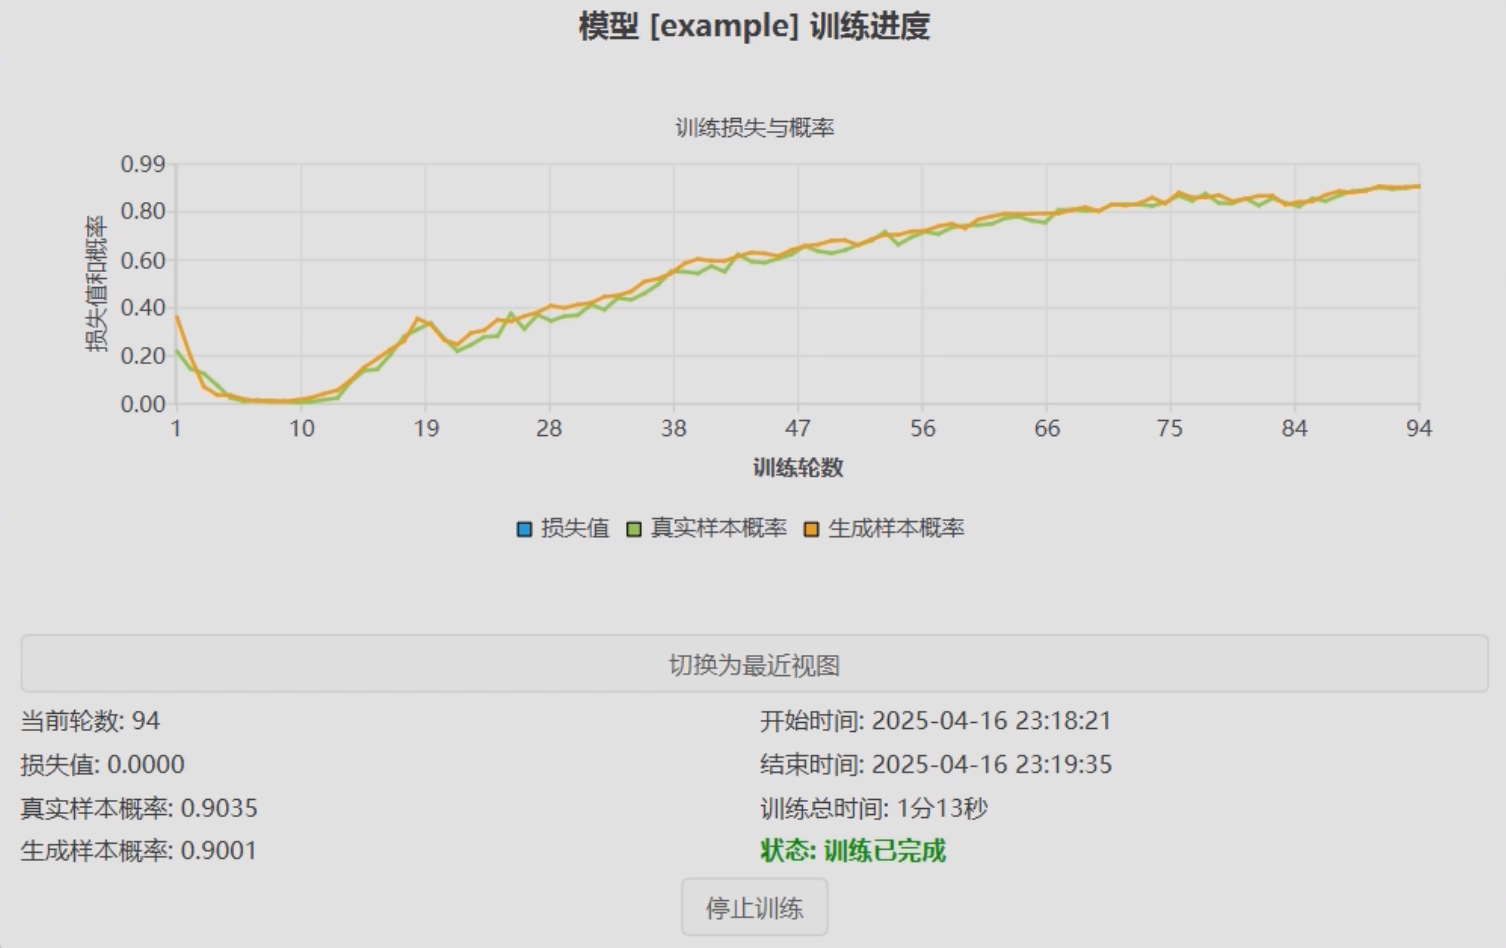
\includegraphics[width=0.80\textwidth]{images/训练进度.png}
    \caption{训练进度}
    \label{训练进度}
\end{figure}

\subsection{缺陷检测模块}

缺陷检测模块是整个缺陷检测系统最重要的组件,负责检测样本与模型的配置,以及对样本进行缺陷识别、可视化、AI辅助分析,最后生成统计报告的完整流程。

(1)检测管理模块

检测管理模块负责配置检测样本组、检测模型。首先是组织和管理检测样本集合及其状态,这部分与样本管理模块类似,如图 \ref{检测界面} 所示,保留了样本组和样本的管理功能,删除了对样本的处理操作,在此不多做赘述。其次就是模型的配置,这部分无需多言。另外,样本组和模型配置完成后,系统会记录并保存到本地,下一次打开项目时自动加载,方便快速恢复检测状态。

\begin{figure}[htb]
    \centering
    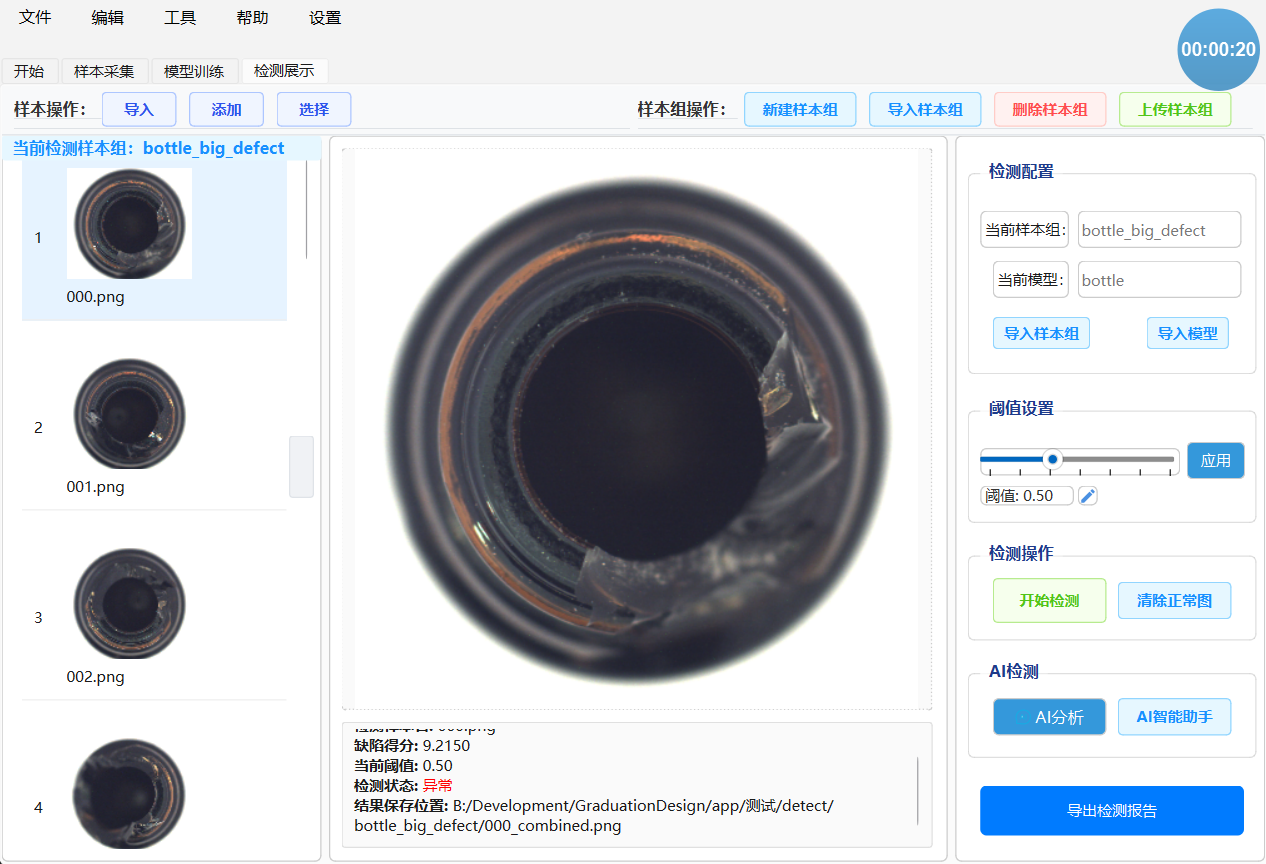
\includegraphics[width=\textwidth]{images/检测界面.png}
    \caption{检测界面}
    \label{检测界面}
\end{figure}

(2)检测模块

检测模块是无监督缺陷检测算法的核心应用环节,负责使用训练好的检测模型对检测样本进行异常区域定位与检测评分,同时将检测结果实时显示在界面预览区域。相似地,在进行实际检测前,系统会自动上传样本组至服务器,并验证样本组和模型组的有效性,比如检测样本组是否上传成功、检测模型是否处于空闲状态等。启动检测后,进入等待态,同时界面显示加载动画,直至获取到第一份检测结果。此时开始进行实时展示,如图 \ref{检测过程} 所示,系统定时从服务器拉取检测数据并实时更新当前结果图以及下方的数据显示栏,同时禁用其余所有组件,以免用户误触。检测结束后,系统自动将检测结果列表保存到本地,此时用户可以在样本列表栏中选择检测项,查看检测结果的详细信息。另外,用户可以依据检测强度的需要,通过滚动条动态调整检测阈值。

检测结果图由原图和异常检测热图组成,对比鲜明,能直观地显示出异常区域的位置和大小。热图以颜色表示异常的概率,颜色越深表示异常的概率越大,反之概率越小。用户点击中央显示框后,可以切换结果图和原图。此外,检测结果图下方显示了当前检测样本的具体信息,包括样本名称、检测时间、检测得分以及检测阈值下的判定状态等。

\begin{figure}[htb]
    \centering
    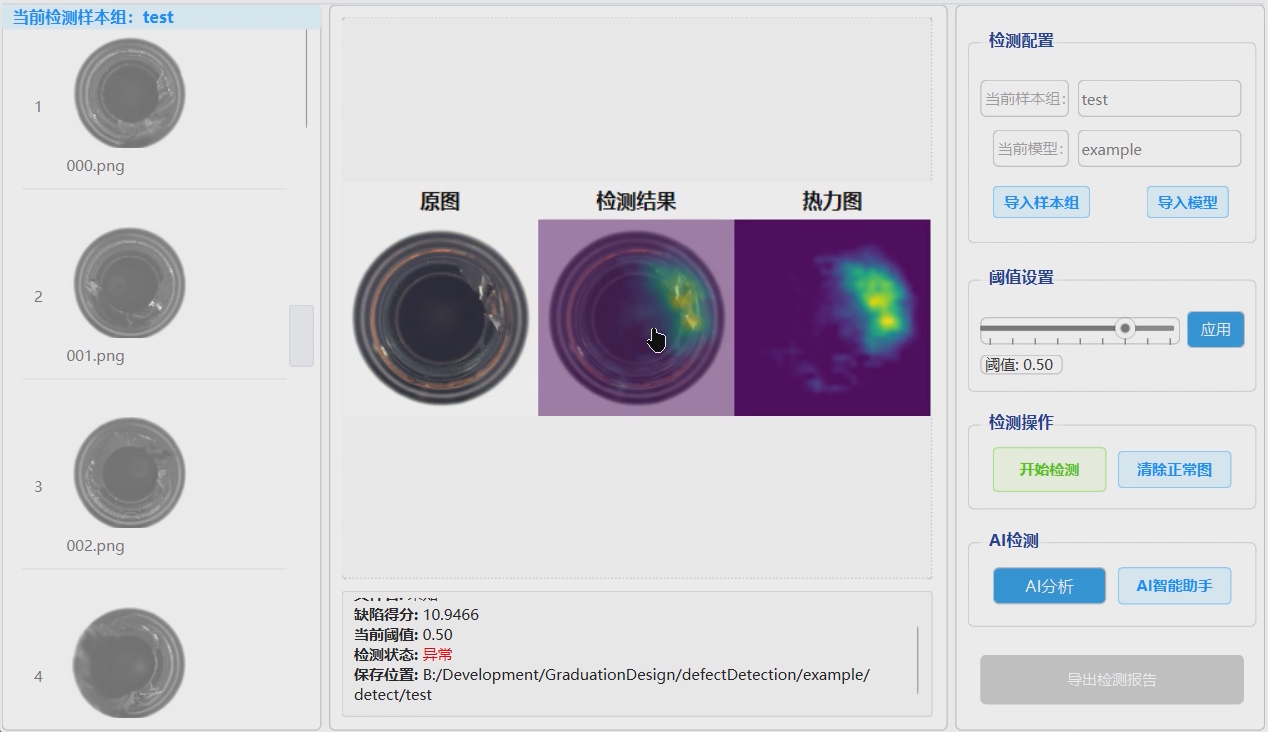
\includegraphics[width=0.82\textwidth]{images/检测过程.png}
    \caption{检测过程}
    \label{检测过程}
\end{figure}

(3)AI辅助分析模块

AI 辅助分析模块是缺陷检测模块的增强组件,融合了大型视觉语言模型(LVLM),弥补了核心缺陷检测算法依赖阈值判定检测结果的不足,同时通过交互式对话界面,提供了异常位置等辅助信息。在检测完成后,用户可选择对其结果存疑的一个或多个样本进行 AI 辅助分析。如图 \ref{AI对话} 所示,用户可以输入缺陷检测相关问题,如图像是否存在缺陷、缺陷的位置,以及描述图像等,在分析完成后系统会自动生成对应的回答。同样地,在 AI 分析启动后,系统进入等待态,显示加载动画,直至处理结束。交互式问答支持对多个分析对象进行连续多轮对话,另外,点击左右导航按钮可以切换分析目标,点击当前分析对象可以切换原图与 AI 分析结果图,这样用户可以直观地对比分析结果。

\begin{figure}[H]
    \centering
    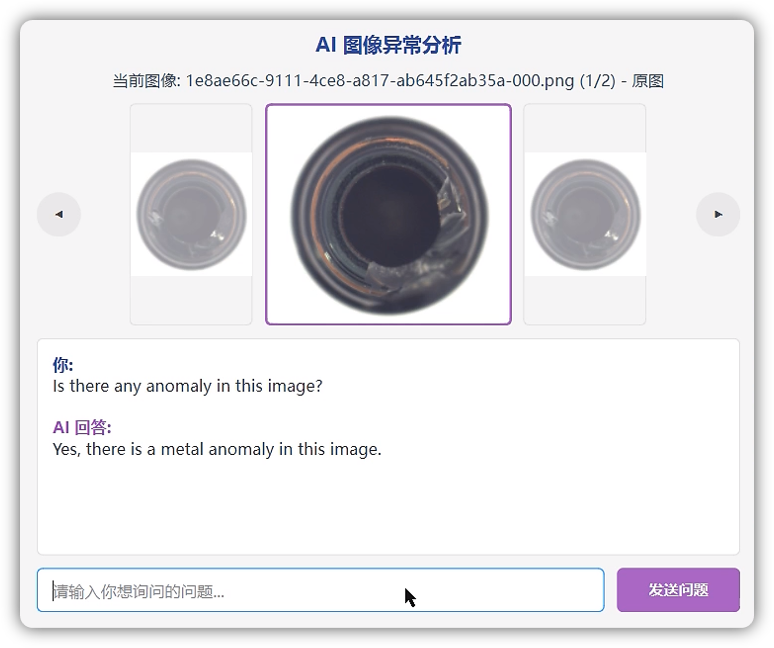
\includegraphics[width=0.58\textwidth]{images/AI对话.png}
    \caption{AI对话}
    \label{AI对话}
\end{figure}

(4)检测报告模块

检测报告模块是缺陷检测模块的总结环节,负责对检测结果进行统计分析,并形成可视化结果报告。在检测完成后,用户可以调整缺陷阈值、聚类参数和块大小,然后点击生成结果报告。报告内容包括检测样本组的基本信息、缺陷位置分析、区域特征统计以及缺陷类型分析。如图 \ref{可视化分析标签页} 所示,当数据解析完成后,用户可以在报告生成界面直接查看可视化结果、统计数据和详细信息,也可以点击下载按钮,将报告以 PDF 格式保存到本地。

\begin{figure}[htb]
    \centering
    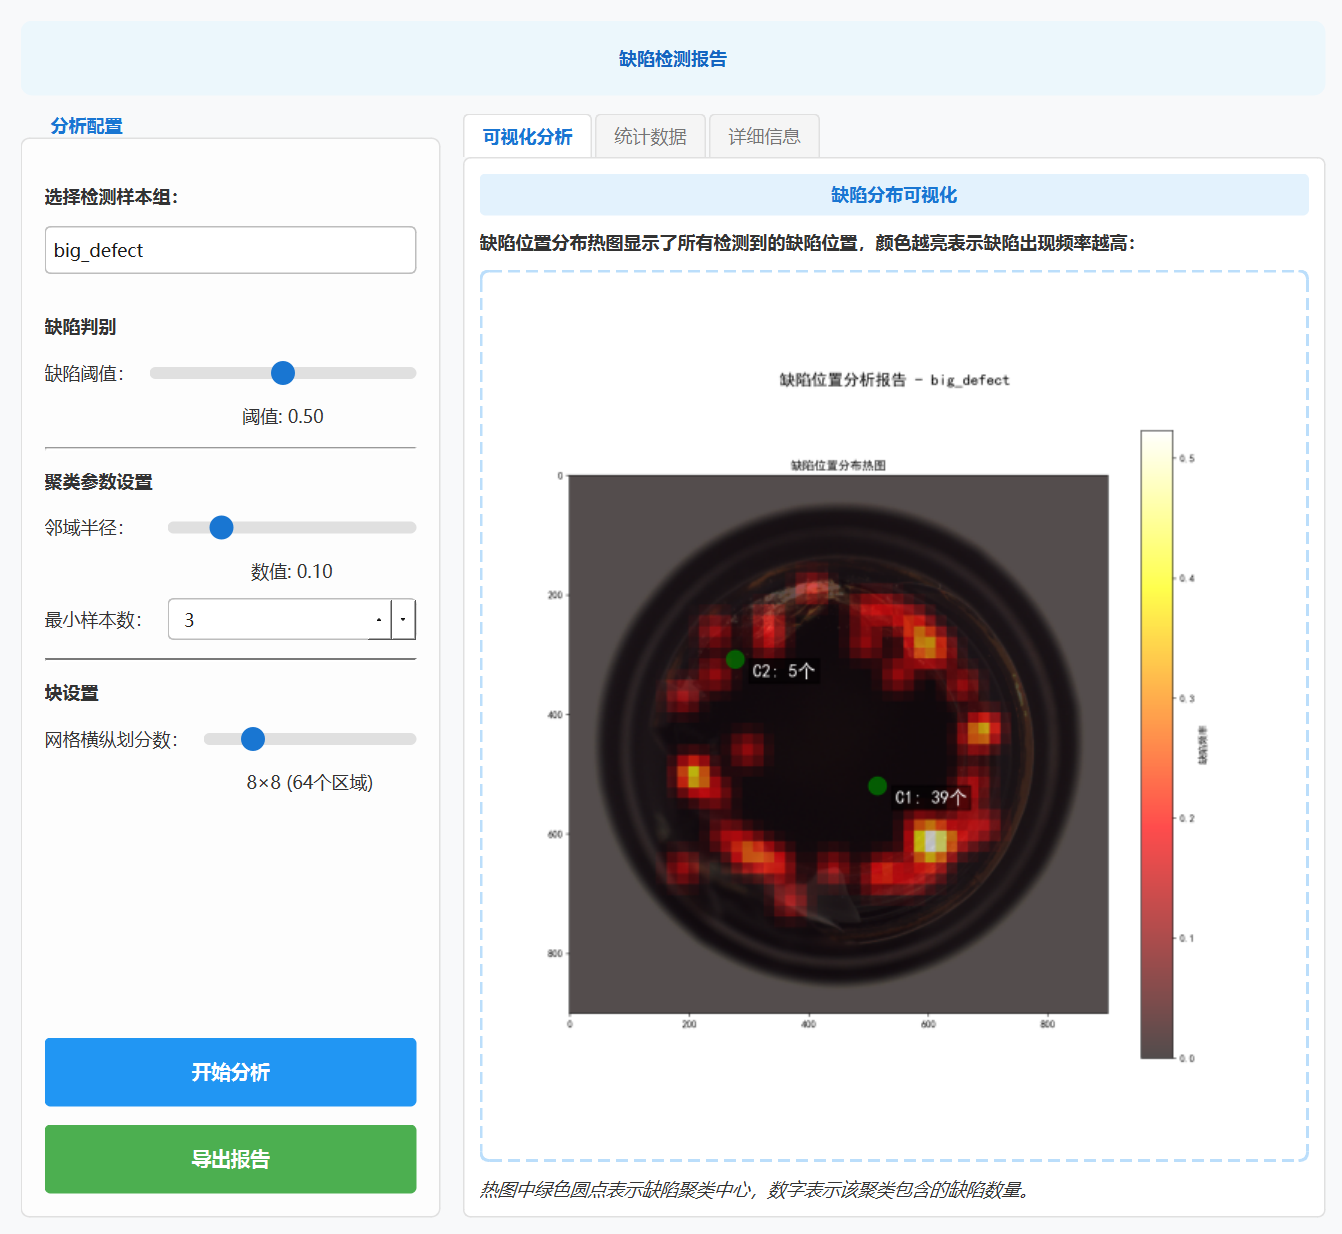
\includegraphics[width=0.88\textwidth]{images/可视化分析标签页.png}
    \caption{可视化分析标签页}
    \label{可视化分析标签页}
\end{figure}


在加载缺陷图像的结果热图后,系统从热图中提取缺陷特征和位置信息。首先,使用 OpenCV 库将检测结果热图转换为灰度图并进行二值化处理,以提取图中的高热区域(缺陷区域)。然后分别处理每个缺陷区域的轮廓,提取其包围框、中心点和轮廓面积等几何特征,用于统计缺陷位置。接着计算有效区域的灰度均值、标准差和最大值,并采用 Sobel 算子计算其梯度均值,用于缺陷纹理分析。至此,得到了缺陷位置和缺陷纹理特征向量。

接下来,对原始图像进行区域特征统计分析。同样地,先使用 OpenCV 库将原图转换为灰度图,并通过热图得出对应原图中的异常区域。然后计算 Sobel 边缘,得到图像梯度幅度。接着,将图像根据指定的块大小划分为均匀的网络,以网格为单位进行统计分析。系统以百分之三十的异常像素比例为标准判断网格是否为异常区域,计算每个网格的灰度均值、灰度方差和边缘密度。最后,根据统计结果,同时结合正常区域和异常区域,得到区域亮度分布直方图、区域纹理复杂度分布直方图和区域边缘密度分布直方图,如图 \ref{区域特征分布图} 所示。亮度分布直方图可用于识别过曝、过暗、局部高反差等亮度异常造成的缺陷;纹理复杂度分布直方图可用于区分纹理断裂、纹理杂乱、纹理缺失等纹理异常导致的缺陷;边缘密度分布直方图则用于识别裂纹、划痕、轮廓缺失等边缘异常所引起的几何特征缺陷。其中,绿色和红色分别代表正常区域和异常区域的分布情况。各图的横坐标分别表示亮度均值、亮度方差、边缘密度,纵坐标表示该特征值的分布情况。亮度均值表示区域内所有像素亮度的平均值,反映整体明暗程度;亮度方差测量区域内像素亮度偏离均值的程度,反映了亮度分布的变化程度,一定程度上反映了纹理复杂度;边缘密度表示区域内边缘像素的比例,反映了缺陷的边缘特征。至于区域亮度直方图为何使用均值,这是因为方差丢失了亮度的绝对水平信息,相同方差的区域可能一个是亮区一个是暗区;同理,区域纹理复杂度直方图使用方差是因为不同纹理复杂度的区域可能有相同的均值,无法区分平滑区域和复杂但亮度平衡的纹理区域。

\begin{figure}[htb]
    \centering
    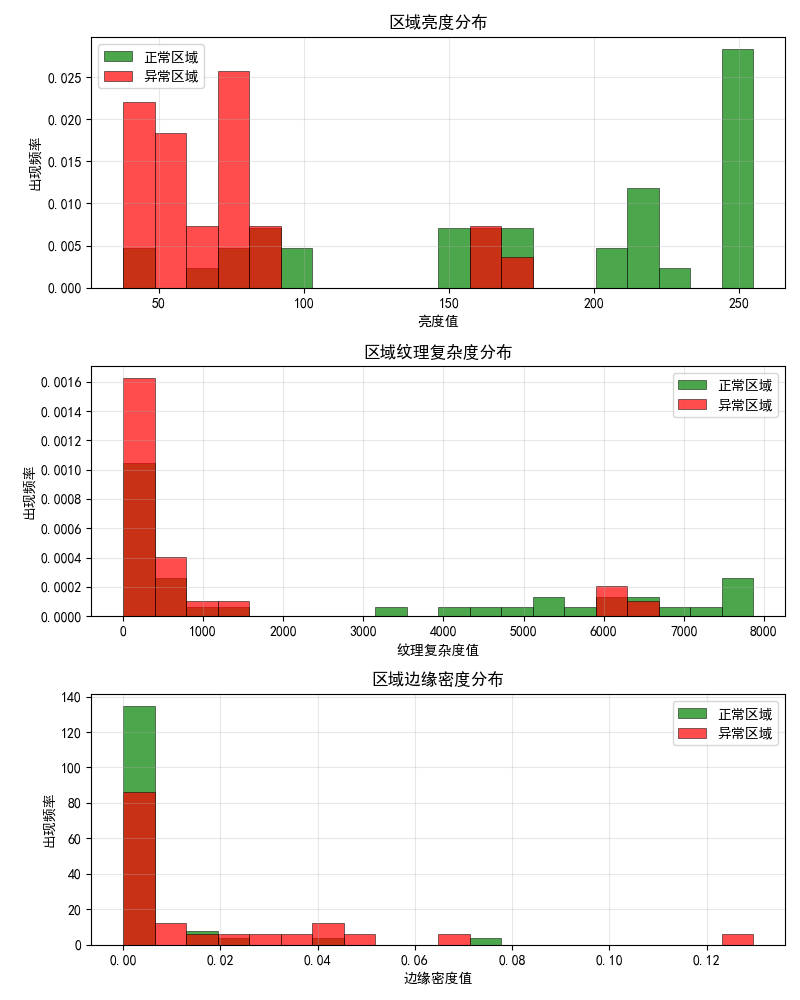
\includegraphics[width=0.6\textwidth]{images/区域特征分布图.png}
    \caption{区域特征分布图}
    \label{区域特征分布图}
\end{figure}

然后,对缺陷位置进行聚类分析,找出缺陷频繁出现的区域。根据指定的邻域半径与最小样本数,使用 DBSCAN 对之前提取的缺陷位置信息进行聚类分析。如图 \ref{可视化分析标签页} 所示,缺陷位置分布图以最佳样本的热图作为背景,将缺陷位置映射到于其上,并使用圆形标记显示聚类结果,便于用户直观地观察缺陷频发区域。

接着,对检测样本的缺陷类型进行统计与分析。参考从热图中提取的缺陷位置和纹理特征向量,根据缺陷亮度阈值以及归一化面积将缺陷分为四个等级,从轻微污染到严重损坏,缺陷程度逐级递增。针对每个缺陷等级,又进一步细分为总共九类具体的缺陷形态,如划痕、裂缝、缺口等。缺陷分类结果使用饼图展示,详见图 \ref{统计数据标签页} 。

\begin{figure}[htb]
    \centering
    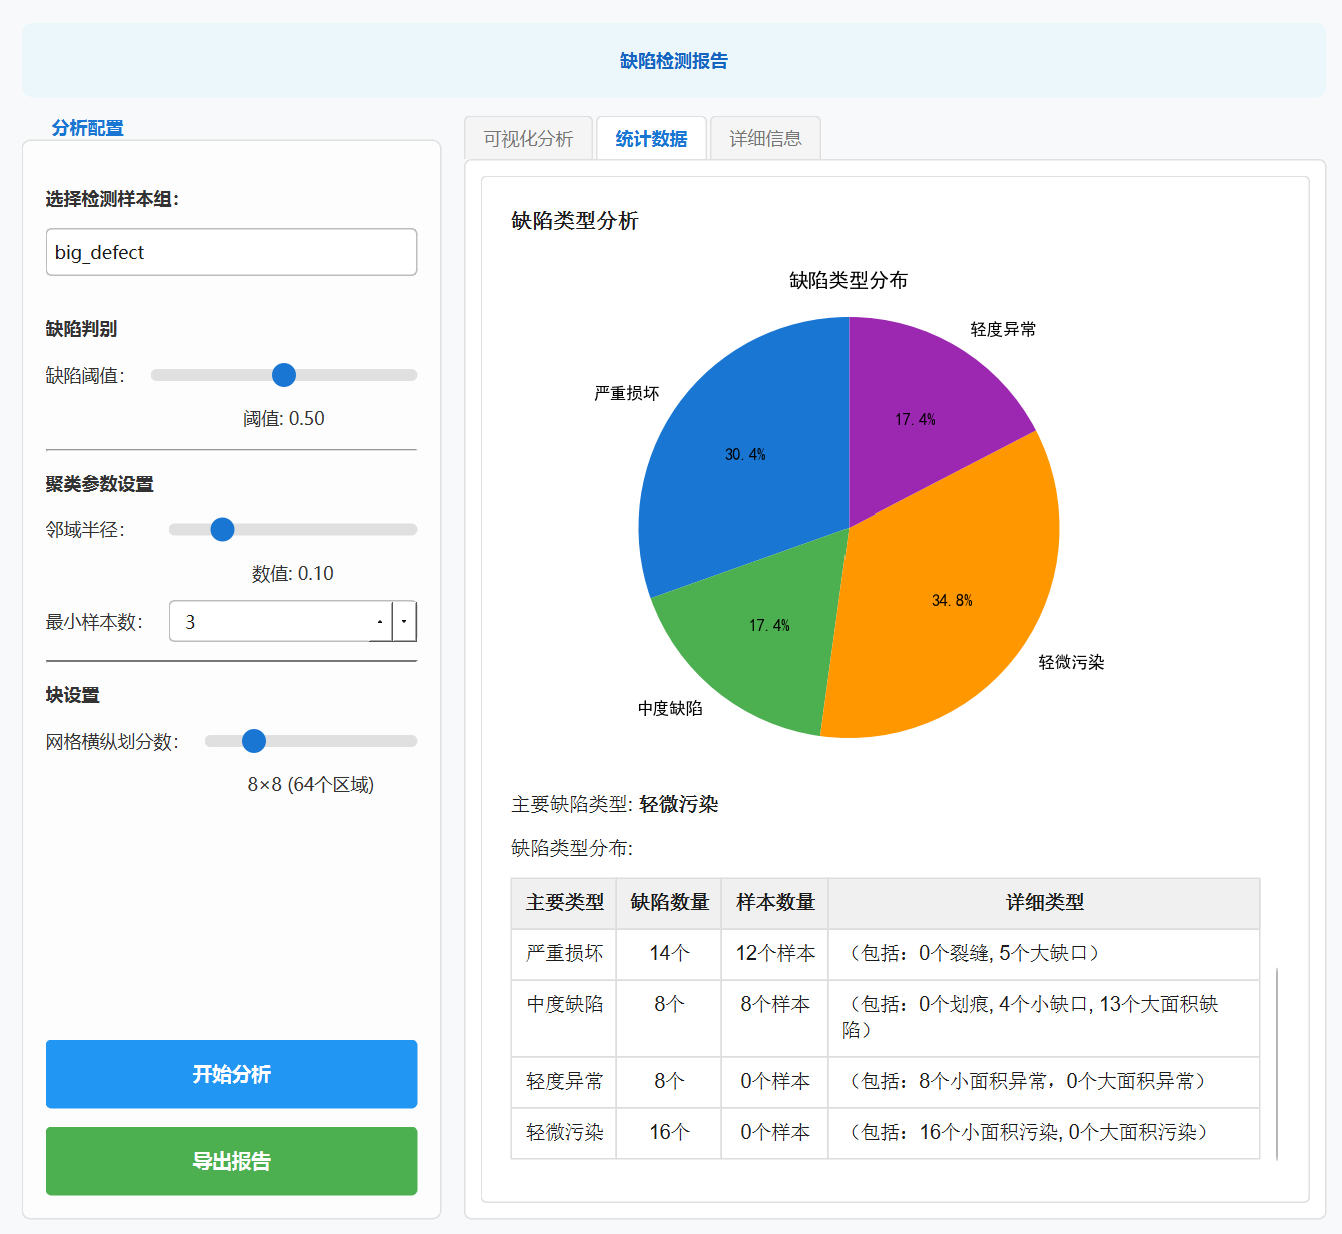
\includegraphics[width=0.88\textwidth]{images/统计数据标签页.png}
    \caption{统计数据标签页}
    \label{统计数据标签页}
\end{figure}

所有分析完成后,系统会通过结构化的报告展示分析结果,用户浏览完毕后可以下载 pdf 报告。检测报告界面包含可视化分析、统计数据、详细信息三个标签页。可视化分析页面主要展示了缺陷位置分布图。统计数据页面共分为五个部分:

\begin{enumerate}
    \item 基本信息,描述了检测样本组的基本信息。
    \item 缺陷位置分析,展示了缺陷的空间分布特点以及聚类结果。
    \item 区域特征统计,对比了正常区域与异常区域在亮度、纹理复杂度和边缘密度三个维度上的差异。
    \item 缺陷类型统计,分析了所有缺陷区域,统计了每类缺陷的细分缺陷数量以及样本数量。
    \item 结论分析,根据前面的统计分析结果给出可能的缺陷原因推断,并提出相应的改进建议。
\end{enumerate}

详细信息页面以树状结构呈现,从基本信息到聚类分析再到缺陷类型统计,每一层级都可以展开查看细节数据,详见图 \ref{详细信息标签页}。

\begin{figure}[H]
    \centering
    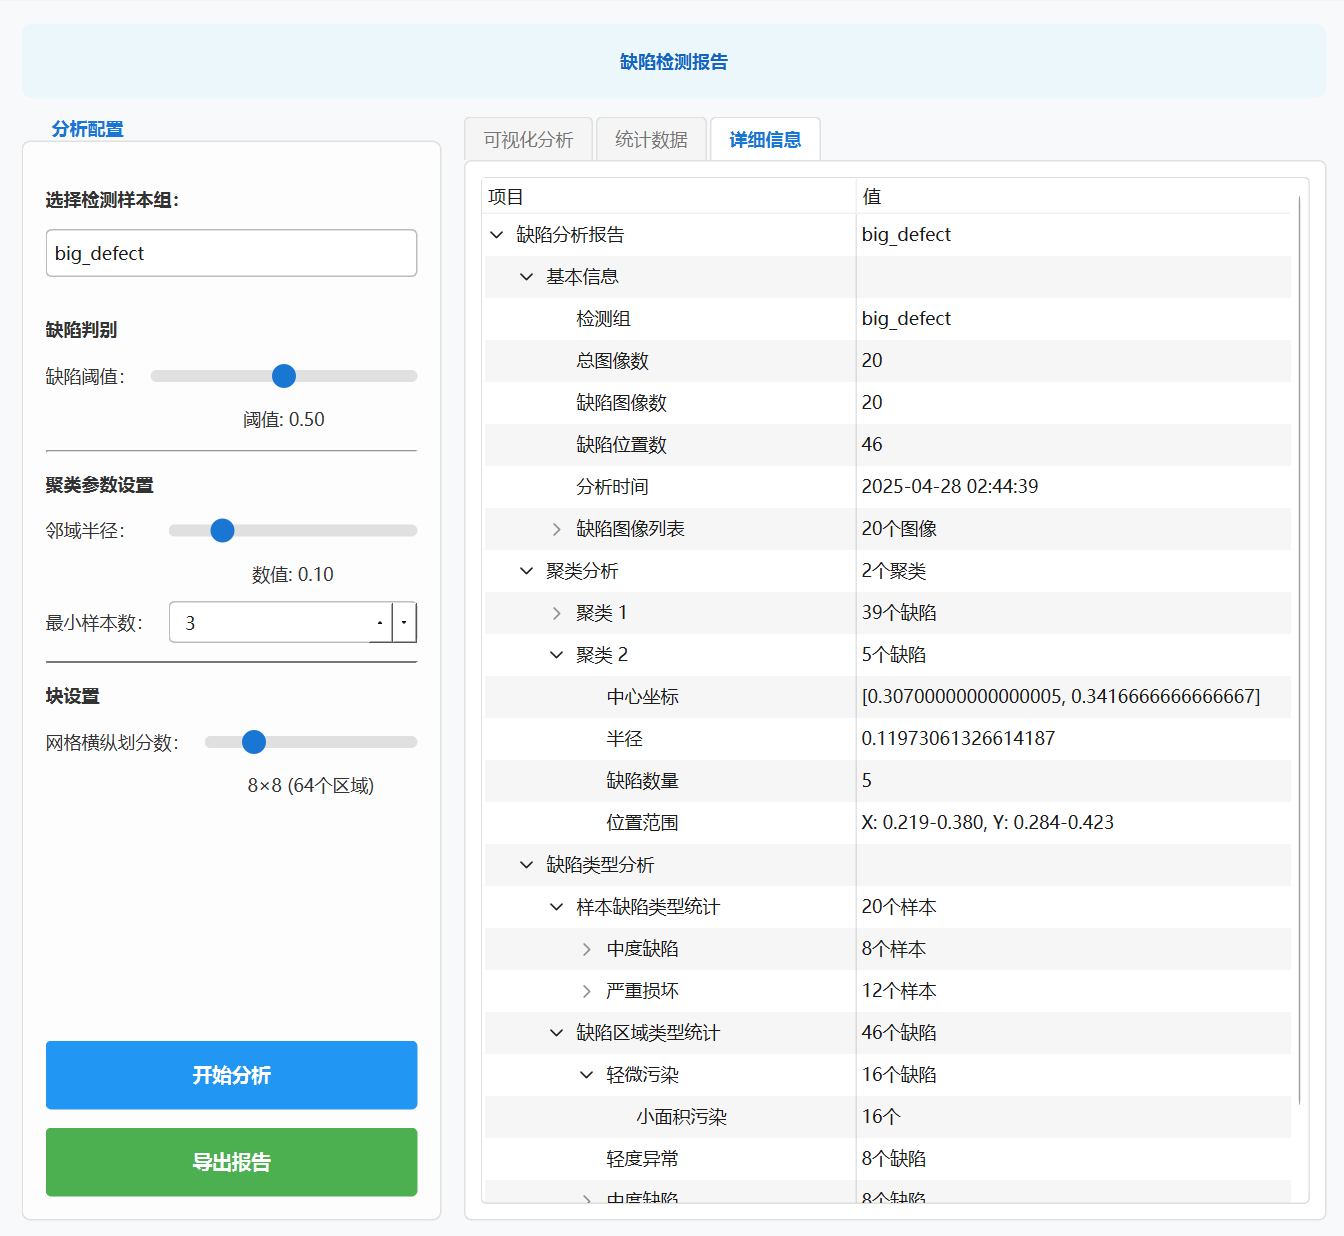
\includegraphics[width=0.88\textwidth]{images/详细信息标签页.png}
    \caption{详细信息标签页}
    \label{详细信息标签页}
\end{figure}

\section{接口与其他}

\subsection{API 接口}

缺陷检测系统通过 HTTP 接口与远程服务器通信,实现模型训练、推理和数据管理等功能,具体 API 如下:

(1) AI 相关 API 如表 \ref{AI_API} 所示。

\begin{table}[H]
    \centering
    \caption{API接口说明}
    \label{AI_API}
    \renewcommand\arraystretch{0.5}
    \begin{tabular}{p{2.5cm}p{3.5cm}p{4cm}p{2.5cm}}
    \toprule[1.5pt]
    API方法 & 功能描述 & 主要参数 & 返回结果 \\
    \midrule[1pt]
    anomaly\_gpt\_infer & 使用大语言模型分析缺陷图像 & img\_list, question, normal\_img\_list, history & 图像分析结果文本列表 \\
    \bottomrule[1.5pt]
    \end{tabular}
\end{table}

(2) 模型相关 API 如表 \ref{model_API} 所示。

\begin{table}[H]
    \centering
    \caption{模型相关API接口说明}
    \label{model_API}
    \renewcommand\arraystretch{0.5}
    \begin{tabular}{p{2.5cm}p{3.5cm}p{4cm}p{2.5cm}}
    \toprule[1.5pt]
    API方法 & 功能描述 & 主要参数 & 返回结果 \\
    \midrule[1pt]
    add\_model & 创建新模型 & name, input\_h, input\_w, end\_acc, layers, patchsize, embed\_dimension & 模型ID \\
    \midrule[0.5pt]
    delete\_model & 删除指定模型 & model\_id & 操作结果 \\
    \midrule[0.5pt]
    update\_model & 更新模型参数 & model\_id, model参数 & 操作结果 \\
    \midrule[0.5pt]
    list\_model & 获取所有模型信息 & 无 & 模型列表 \\
    \midrule[0.5pt]
    get\_model\_id & 根据名称获取模型ID & model\_name & 模型ID \\
    \midrule[0.5pt]
    get\_model & 获取模型完整信息 & model\_name & 模型信息 \\
    \midrule[0.5pt]
    get\_model\_status & 获取模型状态 & model\_name & 状态码(0-3) \\
    \midrule[0.5pt]
    train\_model & 启动模型训练 & model\_id, group\_id & 训练任务信息 \\
    \midrule[0.5pt]
    finish\_model & 手动终止训练 & model\_id & 操作结果 \\
    \midrule[0.5pt]
    train\_info & 获取已训练图像列表 & model\_id & 图像名称列表 \\
    \midrule[0.5pt]
    train\_process & 获取训练实时数据 & model\_id & 训练曲线数据 \\
    \midrule[0.5pt]
    infer\_model & 启动模型推理 & model\_id, group\_id & 推理任务信息 \\
    \midrule[0.5pt]
    infer\_info & 获取已推理图像列表 & model\_id & 图像信息列表 \\
    \midrule[0.5pt]
    infer\_process & 获取推理实时进度 & model\_id & 推理进度信息 \\
    \bottomrule[1.5pt]
    \end{tabular}
\end{table}

(3) 样本组相关 API 如表 \ref{sample_API} 所示。

\begin{table}[H]
    \centering
    \caption{样本组相关API接口说明}
    \label{sample_API}
    \renewcommand\arraystretch{0.5}
    \begin{tabular}{p{2.5cm}p{3.5cm}p{4cm}p{2.5cm}}
    \toprule[1.5pt]
    API方法 & 功能描述 & 主要参数 & 返回结果 \\
    \midrule[1pt]
    upload\_sample & 上传单个样本 & file\_path, group\_id & 服务器文件名 \\
    \midrule[0.5pt]
    download\_sample & 下载样本课题件 & filename & 二进制图像数据 \\
    \midrule[0.5pt]
    get\_sample\_list & 获取组内样本列表 & group\_id & 样本名称列表 \\
    \midrule[0.5pt]
    add\_group & 创建新样本组 & group\_name & 组ID \\
    \midrule[0.5pt]
    delete\_group & 删除样本组 & group\_id & 操作结果 \\
    \midrule[0.5pt]
    clear\_group & 清空样本组内容 & group\_id & 操作结果 \\
    \midrule[0.5pt]
    get\_group\_list & 获取所有样本组 & 无 & 样本组列表 \\
    \midrule[0.5pt]
    get\_group\_id & 根据名称获取组ID & group\_name & 组ID \\
    \bottomrule[1.5pt]
    \end{tabular}
\end{table}


\subsection{其他}

(1)异步处理进度显示与加载动画

缺陷检测系统采用异步处理机制实现耗时操作的实时反馈,有效解决了 UI 阻塞问题,保证在执行复杂任务或进行网络通信时保持响应性,给予用户流畅的操作体验。异步操作反馈大体分为两种,其一是采用 ProgressDialog 显示处理进度,其二是采用 LoadingAnimation 显示加载动画。

ProgressDialog 类封装了 Qt 进度对话框,支持文本提示、百分比显示和取消操作,详见图 \ref{加载进度} 。它适用于可以显示具体处理进度的操作,如上传样本,每上传一个样本更新一次进度,使用户可以直观地看到上传情况。对于耗时长的操作,如生成检测报告,系统采用多阶段进度显示,在各个处理阶段更新进度信息和描述文本。

\begin{figure}[htb]
    \centering
    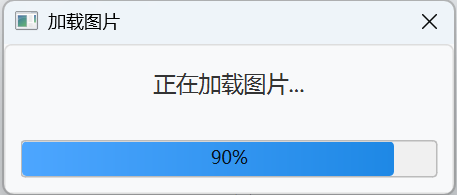
\includegraphics[width=0.3\textwidth]{images/加载进度.png}
    \caption{加载进度}
    \label{加载进度}
\end{figure}

LoadingAnimation 类基于 GIF 动图实现,支持文本提示和动画显示,详见图 \ref{加载动画} 。它适用于如大模型推理这种无法判断剩余时间的操作。具体实现方式是将操作移到异步线程中执行,主线程中显示加载动画,为用户提供视觉反馈,避免其产生卡顿的感觉。

\begin{figure}[htb]
    \centering
    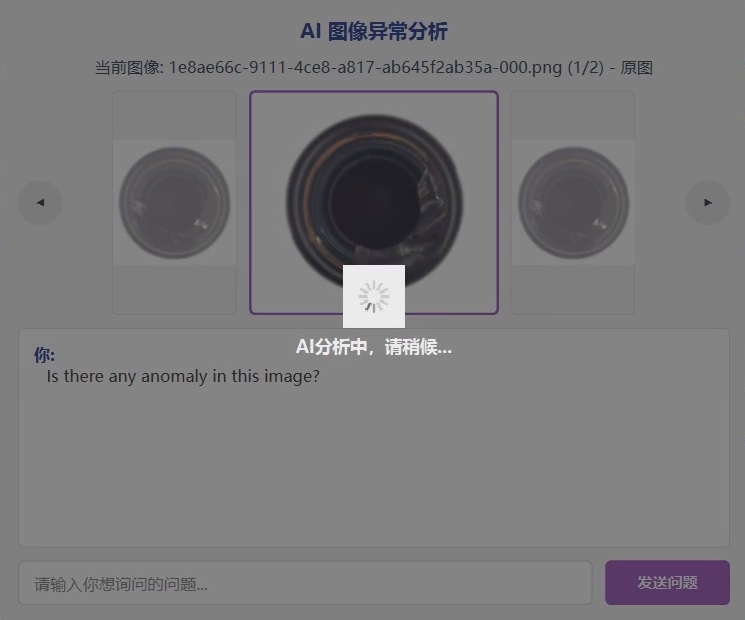
\includegraphics[width=0.58\textwidth]{images/加载动画.png}
    \caption{加载动画}
    \label{加载动画}
\end{figure}

(2)事件过滤器处理点击事件

系统采用 Qt 的事件过滤器(Event Filter)组件处理点击事件。例如 AI 分析模块中的交互式图像查看,用户点击当前图像即可无缝切换原图和结果图,方便进行直观地对比。事件过滤器可以对特定组件的事件流进行拦截,进而实现自定义处理。这种非侵入式的设计将处理逻辑与 ui 组件解耦,增强了系统的扩展性。

(3)点击空白处完成编辑

原方案中使用事件过滤器监听编辑框的 FocusOut 事件,但是给编辑框绑定的 installEventFilter 无法捕捉到焦点失去,因此方案无效。最终解决办法是将编辑框的父组件的 focusPolicy 设置为 Qt::ClickFocus,这样当用户点击父组件空白区域时,编辑框会自动失去焦点,而编辑框的 editingFinished 信号在按下回车键或失去焦点时触发,因此将该信号与完成编辑功能绑定,即可实现点击空白处完成编辑。

(4)流程引导

流程引导是系统的一项辅助功能,介绍了系统的各个功能模块和操作流程,以帮助非专业用户了解缺陷检测的工作流程,达到快速上手的目的。在用户创建或打开项目后就可进入流程引导界面,如图 \ref{流程引导界面} 所示。引导界面采用分流式设计,清晰地展示了系统的两种使用路径:其一是采集样本并对其预处理,然后创建新模型进行训练,训练完成后执行检测;其二是直接使用已有的模型进行检测,然后使用 AI 辅助分析,最后生成检测报告。

\begin{figure}[htb]
    \centering
    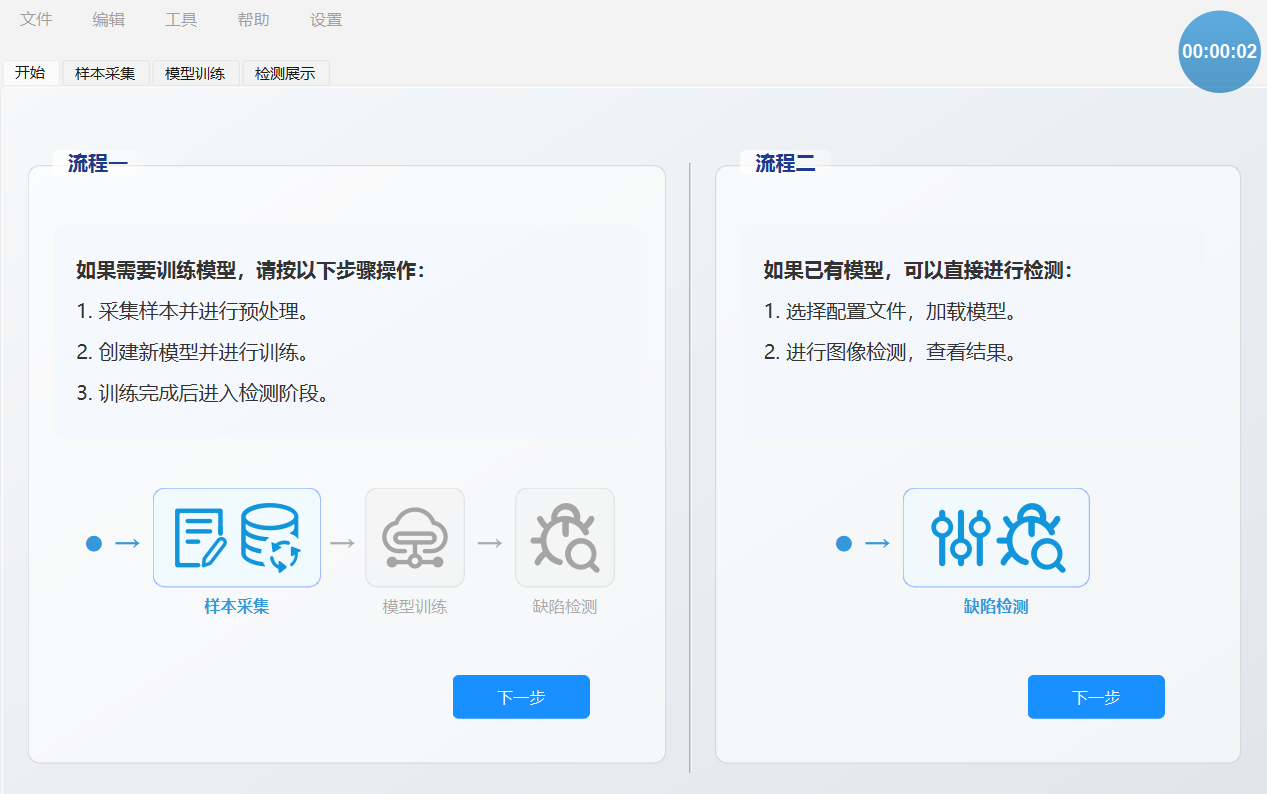
\includegraphics[width=0.88\textwidth]{images/流程引导界面.png}
    \caption{流程引导界面}
    \label{流程引导界面}
\end{figure}

(5) 人机交互启发式原则在系统中的体现

\begin{enumerate}
    \item 帮助和文档:系统在用户打开项目后会显示流程引导。
    \item 依赖识别而非记忆:系统界面上的每个按钮都配有直观可识别的图标。
    \item 一致性和标准化:系统采用统一的 UI 设计,确保不同界面的布局和样式风格保持一致。
    \item 系统状态可见度:系统通过加载进度和加载动画来反馈操作的处理情况。
    \item 系统和现实世界的吻合:系统的缺陷检测流程模拟了现实中样本采集、模型训练、缺陷检测、AI辅助分析和报告生成的过程,类似于工人观摩样本、肉眼检测缺陷、高级质检人员辅助分析及手动书写报告的实际操作。
    \item 避免出错:系统在检测时会禁用界面上的组件以限制用户行为。
    \item 帮助用户识别、诊断和恢复错误:系统通过弹窗显示错误信息,例如在新建项目时输入名称格式非法时进行提示。
    \item 使用的灵活性和高效性:系统支持用户拖拽文件打开项目;用户新建样本组或模型时可直接按回车键确认;用户切换页面时系统自动检查是否上传样本组、是否训练模型。
\end{enumerate}

\section{部署}

\subsection{服务器端部署}

服务器由哈工大多模态智能及应用研究中心支持,项目运行于 ubuntu 22.04 环境,将服务器端打包为镜像后可快速部署于任意服务器上运行。

\subsection{客户端部署}

客户端通过 PyInstaller 将源代码、ui 文件和库文件打包为 .exe 格式的可执行文件,并部署在 Windows 操作系统上运行。需要注意的是,在使用 PyInstaller 打包时,需要显式地导入 OpenCV 库和 ui 文件夹。另外,在运行应用程序时,界面的图片可能无法正常显示,这是因为可执行文件的工作目录与 ui 文件夹的相对位置发生了变化。系统采取的解决办法是在程序启动时将工作目录动态设置为应用程序所在的目录。

\section{本章小结}

本章对缺陷检测系统的实现过程,从开发环境到十一个子模块的实现再到部署落地方案,均进行了系统性阐述。另外,本章还介绍了系统里一些用于优化用户体验的处理,如异步处理、事件过滤器、裁剪功能和流程引导等,它们严格遵循了人机交互的八大启发式原则,使系统变得友好、高效、易用。

\chapter{实验}

\section{数据集}

我们在 MVTec AD\cite{[16]} 数据集上进行测试,该数据集用于工业领域的无监督缺陷检测,包含 5354 张不同物体和纹理类别的高分辨率彩色图像。MVTec AD 共有 15 个不同的产品类别,每个类别包括一组无缺陷的训练集,和一组包含各种缺陷的图像以及无缺陷的图像的测试集。这 15 个类别又可细分为 5 种纹理图,如铁丝网、皮革、瓷砖等,和 10 种物体图,如瓶子、电缆、胶囊、榛子、金属螺母等。如图 \ref{MVTec} 所示,每个类别都给出了一个正常图像、异常示例和异常区域的特写视图。它们共包含 73 种不同类型的缺陷,如划痕、凹痕、污染和各种结构变化。

\begin{figure}[htb]
    \centering
    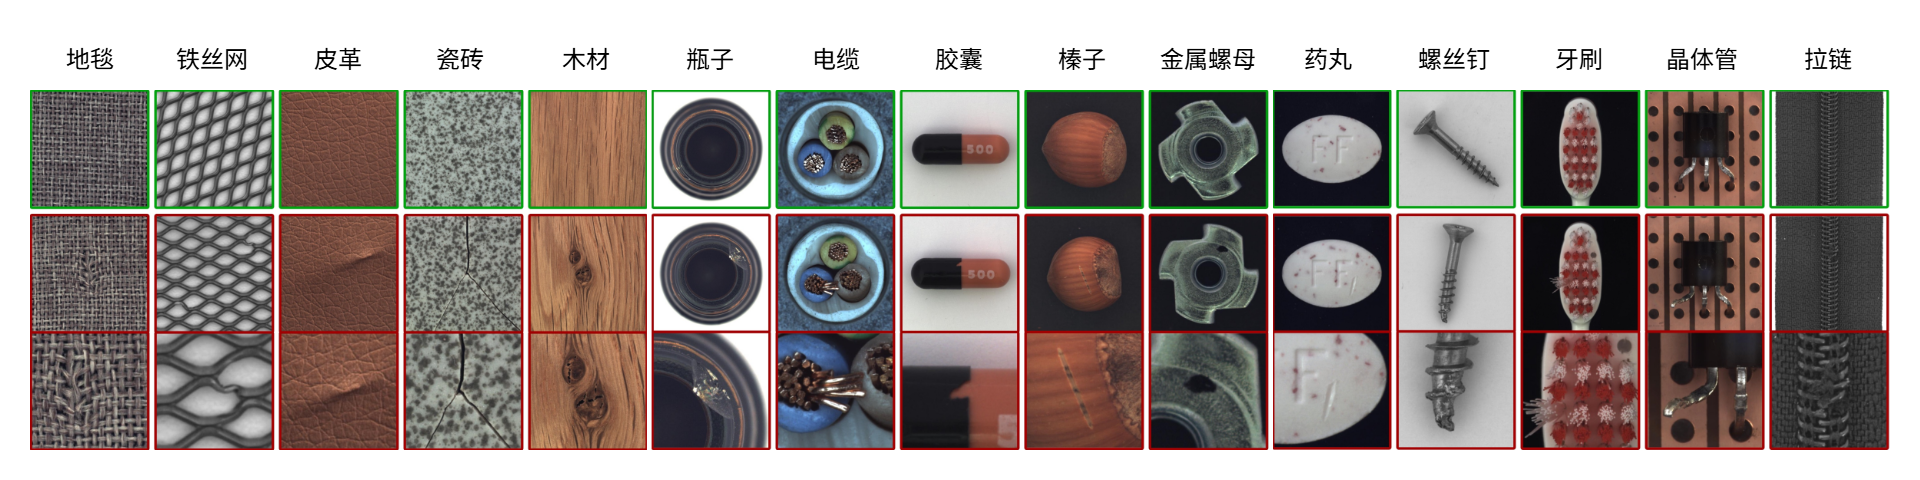
\includegraphics[width=0.88\textwidth]{images/MVTec.png}
    \caption{MVTec AD 数据集的五个纹理和十个对象类别的示例图像}
    \label{MVTec}
\end{figure}

\section{评估指标}

受试者工作特征曲线下面积(Area Under the Receiver Operating Characteristic curve,AUROC)是异常检测和二分类任务中常用的评估指标,反映了模型在不同判别阈值下的整体分类性能。AUROC 的取值范围是 [0, 1],越接近 1 表示模型区分正常和异常的性能越好;若 AUROC 为 0.5,则与随机猜测无异。

I-AUROC(Image-level AUROC) 和 P-AUROC(Pixel-level AUROC) 是工业缺陷检测领域常用的细化评估指标,分别表示图像级和像素级的 AUROC。前者以整张图像为单位,判定正常或异常,适用于评估模型在实际生产中对产品合格与否的整体判断能力;后者以像素为单位,判定每个像素是否属于异常区域,适用于评估模型检测缺陷具体位置和形状的能力。

\section{实验设计}

我们首先在 MVTec AD 数据集上随机挑选了一个对象类别 capsule,用于测试基于 SimpleNet 的无监督异常检测模型,并使用 I-AUROC 和 P-AUROC 以及 SPEED 作为评估指标,比较了不同精度选择和速度选择下的检测效果。然后,为了方便观测结果起见,我们以便于人工定位缺陷的 bottle 数据集为例,测试了基于 AnomalyGPT 的辅助分析中检测缺陷是否存在和缺陷位置的准确率。

\section{结果分析}

\subsection{SimpleNet 异常检测}

缺陷检测结果如表 \ref{acc_level_comparison} 所示,ACC\_LEVEL 为所选精度级别,TIME 为单张样本检测耗时。可以看出,选择精度越高,I-AUROC 越高,但检测每个样本耗时越长。P-AUROC 在精度选择为中等时达到最高,这是由于过高精度模型可能在特征提取时过度关注局部细节,导致在像素级别上产生的误判更多,即对细微纹理的变化过度敏感。另外,高精度模型的处理速度明显下降(0.1s/个),这表明精度选择高时模型复杂度显著增加,但检测精度提升有限。而在工业场景中,要平衡检测速度和检测精度,所以一般默认选择中等精度即可。如表 \ref{speed_level_comparison} 所示,SPEED\_LEVEL 为所选速度级别。在默认中等精度的情况下,I-AUROC 随着速度等级的提高而降低,由于速度选择是对原来的参数配置做的细微调整,因此 I-AUROC 和样本检测耗时变化不大。另外,P-AUROC 的变化再次验证了前文的结论。

\begin{table}[H]
    \centering
    \caption{不同精度级别下异常检测的性能对比。}
    \label{acc_level_comparison}
    \renewcommand\arraystretch{0.5}
    \begin{tabular}{c|c|c|c}
    \toprule[1.5pt]
    ACC\_LEVEL & I-AUROC & P-AUROC & TIME(ms) \\
    \midrule[1pt]
    LOW & 90.35\% & 98.38\% & 16.55 \\
    \midrule[0.5pt]
    MEDIUM & 98.40\% & 98.83\% & 21.91 \\
    \midrule[0.5pt]
    HIGH & 99.48\% & 98.07\% & 102.77 \\
    \bottomrule[1.5pt]
    \end{tabular}
\end{table}

\begin{table}[H]
    \centering
    \caption{不同速度级别下异常检测的性能对比。}
    \label{speed_level_comparison}
    \renewcommand\arraystretch{0.5}
    \begin{tabular}{c|c|c|c}
    \toprule[1.5pt]
    SPEED\_LEVEL & I-AUROC & P-AUROC & TIME(ms) \\
    \midrule[1pt]
    HIGH & 96.85\% & 98.55\% & 21.79 \\
    \midrule[0.5pt]
    MEDIUM & 98.40\% & 98.83\% & 21.91 \\
    \midrule[0.5pt]
    LOW & 99.16\% & 98.78\% & 23.12 \\
    \bottomrule[1.5pt]
    \end{tabular}
\end{table}


\subsection{AnomalyGPT 辅助分析}

如表 \ref{AI_detection_accuracy} 所示,DEFECT\_CLASS 为样本缺陷类别,EXISTANCE\_ACC 为异常存在性准确率,POSITION\_ACC 为缺陷位置准确率。在 bottle 测试集的三类样本中,AnomalyGPT 辅助分析异常是否存在的准确率都达到了 100\%,效果非常出色。但它在分析缺陷位置的准确率上表现一般,尤其是在缺陷较大的样本中,准确率仅为 70\%。这说明 AnomalyGPT 在辅助分析时,容易被大范围的异常区域所干扰,不能准确地定位缺陷位置。本课题在实验过程中发现,出现错误最多的场景是当检测到瓶底四周都存在异常时,AnomalyGPT 会认为缺陷位于瓶底中心处,这可能是 AnomalyGPT 需要改进的地方。

\begin{table}[H]
    \centering
    \caption{不同缺陷类别下 AI 辅助判定缺陷存在性与定位缺陷的性能。}
    \label{AI_detection_accuracy}
    \renewcommand\arraystretch{0.5}
    \begin{tabular}{c|c|c}
    \toprule[1.5pt]
    DEFECT\_CLASS & EXISTANCE\_ACC & POSITION\_ACC \\
    \midrule[1pt]
    GOOD & 100\% & - \\
    \midrule[0.5pt]
    SMALL\_DEFECT & 100\% & 86.3\% \\
    \midrule[0.5pt]
    BIG\_DEFECT & 100\% & 70\% \\
    \bottomrule[1.5pt]
    \end{tabular}
\end{table}

\section{本章小结}

本章对缺陷检测系统进行了实验。首先,介绍了实验用到的 MVTec AD 数据集和用于评估的指标。然后,设计实验验证了 SimpleNet 异常检测模型在不同精度和速度选择下的结果,同时检测了 AnomalyGPT 辅助分析模型在判定异常是否存在和定位缺陷位置的效果。最后,对实验结果进行了分析,证明了精度与速度选择的设定是合理的。

\chapter{总结与展望}

\section{工作总结}

本课题针对工业缺陷检测中存在的标注数据稀缺、缺陷多样化、现有系统操作及配置复杂等问题,设计并实现了基于无监督深度学习的工业缺陷检测系统。系统以无监督检测方法 SimpleNet 为核心,结合 AnomalyGPT 大型视觉语言模型的辅助分析能力,实现了样本管理、模型训练和缺陷检测三大功能模块。在样本管理阶段,系统通过动态样本组管理和样本预处理操作解决了实际工业场景中样本质量参差不齐和样本量少的问题。在模型训练阶段,系统既保留了手动配置参数的方式以满足专业用户的研究需求,又创新性地使用了参数映射,将复杂的深度学习参数抽象为“精度-速度-缺陷大小”等直观选项呈现给用户,降低了非专业用户的操作门槛。在缺陷检测阶段,系统融合了 SimpleNet 的高效异常检测能力与 AnomalyGPT 的自然语言交互能力,通过可视化的结果热图、AI 辅助分析、缺陷检测报告的形式,实现了从缺陷定位到工艺优化的全流程支持。实验结果表明,系统在 MVTec AD 数据集上表现优异。默认情况下 SimpleNet 模型在检测胶囊类样本的 I-AUROC 达到 98.4\%,每张图像平均检测时间为 22ms 左右;AnomalyGPT 对异常存在性的判定准确率达到 100\%。此外,系统采用 Qt 框架实现了跨平台部署,使用异步处理机制保障了界面响应速度与稳定性,同时参照人机交互启发式原则对系统交互界面进行了优化设计,最终实现了一款具有高效性、易用性和可解释性的工业质检工具,为智能化工业制造中的缺陷检测提供了高效且实用的解决方案。

\section{未来展望}

尽管缺陷检测系统在检测精度和实用性方面取得了良好效果,但存在着诸多不足之处仍亟待解决。未来检测系统的改进方向主要包括改造系统框架、优化检测算法、完善系统功能、升级系统架构和促进工业落地这几个方面。首先,可探索多种算法融合框架,实现不同场景下用户对工业产品检测算法的动态选择。其次,可尝试半监督方法,结合有监督与无监督深度学习的优势,以少量标注数据提升缺陷检测的性能。再者,可考虑扩展系统的输入,支持多模态数据来进行融合分析,如红外、超声波等其它传感器数据,并结合生产需求增设实时检测模式。然后,可尝试应用分布式数据库优化和云端协同计算,提升系统应对海量数据的处理能力,同时构建用户权限管理和数据共享机制,增强企业级应用的协作能力。最后,可探讨与企业合作,对细化的制造领域进行专项优化,获取相关领域的数据对大模型进行微调,并完善 AI 辅助分析和缺陷检测报告,增强系统对生产工艺优化的支持,以期做到真正的智能化制造。

%---------------------------------------------------------------------
%	参考文献
%---------------------------------------------------------------------

% 生成参考文献页
\printbibliography

%---------------------------------------------------------------------
%	致谢
%---------------------------------------------------------------------

\begin{acknowledgement}
    
    感谢葛季栋教授、邬向前教授以及马丁老师对毕业设计和论文的指导。
    感谢张砚钦师兄、史云浩师兄在日常生活和毕业设计的帮助。
    
    光阴似箭,日月如梭。四年时间,转瞬即逝。回首往昔,感慨万千。
    
    感谢唐熙童兄弟、刘雨欣同志在大学生涯的相处陪伴。
    感谢陈虹钢兄弟、谢志鹏老哥在保研路上的指点。
    感谢和罗晗、兰天宇、李怡龙、赵子贤、彭嘉锐室友,以及王渤元、曲廷锌等同学在南京大学四年里共渡的欢乐时光。
    
    千日太匆匆,还如一梦中。而今别君去,十年难相逢。
    
    感谢和廖凡、王薏萌、柴雨舟、刘锐婕等同学在重庆市南开中学三年里共渡的欢乐时光。
    感谢和王梅岭、何玉琪、王瑞祥、徐文阔等同学在重庆市育才中学三年里共渡的欢乐时光。
    感谢和付卫东、隆昌顺、谢昌林、周灏等同学在重庆市大学城人民小学四年里共渡的美好时光。
    
    十年寒窗成回首,百般滋味待丰收。一纸文书一场梦,几家欢喜几家愁。
    
    感谢和陈远栋、安翔龙等同学在深圳市龙岗区坪地一小两年里共渡的美好时光。
    感谢和李官正、袁佳忆等兄弟在坪地渡过的童年时光。
    感谢父母、爷爷奶奶、外公外婆和家人们这二十年来的养育和陪伴。
    
    儿时岁悠悠,人生不胜愁。不求人长乐,但愿心长留。

\end{acknowledgement}

%---------------------------------------------------------------------
%	学术简历
%---------------------------------------------------------------------

% 详见手册中"成果列表"一节
% \njuchapter{学术成果}
% \njupaperlist[攻读博士学位期间发表的学术论文]{preskill2018}

%---------------------------------------------------------------------
%	附录部分
%---------------------------------------------------------------------

% 附录部分使用单独的字母序号
% \appendix

% 可以在这里插入补充材料
% \chapter{正文中涉及的数据及源代码}
% \section{系统主要功能模块示例代码}

% 完工
\end{document}
